% Copyright (c) 2016, Mario Preishuber. All rights reserved.
%
% Notation: <option description> (<options>)
%
% Specify
%   - layout (onecolumn, twocolumn),
%   - thesis type (bachelor, master),
%   - language (english, naustrian)
%   - indicate that you want to use the university seal as background of the
%     titlepage (seal)
%   - indicate that you want signature fields (signatures)
%   - chapter headings to be on the next page or the next recto, verso page
%     (openany, openright, openleft) (standard memoir option, passed through)
\documentclass[onecolumn, openright, master, english, signatures]{dbrgrptt}
\usepackage[nameinlink]{cleveref}
\usepackage{listings}
\usepackage{multirow}
\usepackage{tikz}
\usetikzlibrary{arrows, positioning, fit}
\tikzset{%
  block node/.style={rectangle,draw,align=center, minimum width=1.5cm, minimum height=1.0cm},
  cpu node/.style={rectangle,draw,align=center, minimum width=1.5cm, minimum height=1.0cm, fill=black!30},
  cache node/.style={rectangle,draw,align=center, minimum width=1.5cm, minimum height=1.0cm, fill=green!30},
}

\definecolor{red}{RGB}{221,17,68}
\definecolor{orange}{RGB}{239,133,53}
\definecolor{yellow}{RGB}{255,202,40}
\definecolor{green}{RGB}{124,168,43}

\tikzstyle{cache-load}=[draw=green, line width=0.5mm, rectangle, rounded corners=0.5mm, minimum size=4mm, scale=0.7]
\tikzstyle{cache-store}=[fill=yellow, draw=yellow, line width=0.5mm, rectangle, rounded corners=0.5mm, minimum size=4mm, scale=0.7]
\tikzstyle{memory-load}=[draw=orange, line width=0.5mm, circle, scale=0.7]
\tikzstyle{memory-store}=[fill=red,draw=red, line width=0.5mm, circle, scale=0.7]



\hypersetup{
    colorlinks=false,
    pdfborder={0 0 0},
}

\begin{document}

%%%%%%%%%%%%%%%%%%%%%%%%%%%%%%%%%%%%%%%%%%%%%%%%%%%%%%%%%%%%%%%%%%%%%%%%%%%%%%%%
% Titling page / Initialization
%%%%%%%%%%%%%%%%%%%%%%%%%%%%%%%%%%%%%%%%%%%%%%%%%%%%%%%%%%%%%%%%%%%%%%%%%%%%%%%%

\thesistitle{%
Towards cache-optimal address allocation:%
% ~How fast could your code have run if you had known where to allocate memory?%
~How slow is your code?
}%
\thesisdate{\today}%
\thesisauthor{Mario Preishuber}{01120643}%
\setsupervisor{Univ.-Prof. Dr. Christoph Kirsch}%

% pages after this command (and before \mainmatter) are numbered roman
\frontmatter%

\hypersetup{pageanchor = false}%

%%%%%%%%%%%%%%%%%%%%%%%%%%%%%%%%%%%%%%%%
% titlepage / Titelseite
\maketitle%

%%%%%%%%%%%%%%%%%%%%%%%%%%%%%%%%%%%%%%%%
% statement of authentication / Verfassungserklaerung
\authenticationstatement%

%%%%%%%%%%%%%%%%%%%%%%%%%%%%%%%%%%%%%%%%
% acknowledgments / Danksagung
\acknowledgments{
Es ist an der Zeit einigen Begleitern auf meinem Weg dankzusagen.
\\~\\
% Christoph Kirsch
Ein großes Dankeschön gebührt meinem Betreuer \emph{Prof. Christoph Kirsch} für die Betreuung durch mein Bachelor- und Masterstudium. Du hast meine Entwicklung voran getrieben und mich stets zu Höchstleistungen motiviert; du hast mir Türen geöffnet von denen ich nicht zu träumen gewagt hätte; für diese wertvollen Erfahrungen möchte ich dir danken.
\\~\\
% Mama & Papa
Am Ende meines Studiums angekommen, möchte ich mich bei meiner \emph{Familie} bedanken. Insbesondere gilt der Dank meinen Eltern, Günther und Helga, für ihr Vertrauen und ihre Unterstützung. Danke, dass ihr mir dieses Studium ermöglicht habt.
\\~\\
% Alexander Miller
Dankeschön auch an \emph{Alexander Miller} für die wertvollen Diskussionen, welche dieses Projekt vorangetrieben haben.
\\~\\
% Thomas Hütter
Abschließend möchte ich mich noch bei \emph{Thomas Hütter} bedanken; für die unzähligen Stunden, die wir mit Projekten verbracht haben.
\\~\\
\textbf{Danke.}
}

%%%%%%%%%%%%%%%%%%%%%%%%%%%%%%%%%%%%%%%%
% abstract / Kurzfassung
\abstract{%
% motivation
The latency of accessing data stored in the main memory is a known problem in computer systems.
% problem statement
We are interested in finding metrics that characterize the performance of a program for a given cache.
% methods & approach
We analyze the characteristic of \emph{load} and \emph{store} instructions, called the \emph{memory access trace}, of two well known benchmark suites, namely SPEC 2006 and V8.
For our analysis about the potential performance improvement in terms of memory access performance and memory usage we modify the addresses used by a memory access trace.
% results & conclusion
Our analysis illustrates that for some benchmarks we are able to improve the memory usage and the memory access performance by a factor of at least two.
Nonetheless, the chosen metrics illustrate tendencies for improvement rather than unique characteristics.
}

%%%%%%%%%%%%%%%%%%%%%%%%%%%%%%%%%%%%%%%%
% table of contents / Inhaltsverzeichnis
\setcounter{tocdepth}{5}
\tableofcontents%

\hypersetup{pageanchor = true}%
%

%%%%%%%%%%%%%%%%%%%%%%%%%%%%%%%%%%%%%%%%%%%%%%%%%%%%%%%%%%%%%%%%%%%%%%%%%%%%%%%%%%%%%%%%%%%%%%%%%%%
% Main content
%%%%%%%%%%%%%%%%%%%%%%%%%%%%%%%%%%%%%%%%%%%%%%%%%%%%%%%%%%%%%%%%%%%%%%%%%%%%%%%%%%%%%%%%%%%%%%%%%%%

\mainmatter%

%%%%%%%%%%%%%%%%%%%%%%%%%%%%%%%%%%%%%%%%%%%%%%%%%%%%%%%%%%%%%%%%%%%%%%%%%%%%%%%%%%%%%%%%%%%%%%%%%%%
%%%%%%%%%%%%%%%%%%%%%%%%%%%%%%%%%%%%%%%%%%%%%%%%%%%%%%%%%%%%%%%%%%%%%%%%%%%%%%%%%%%%%%%%%%%%%%%%%%%
%%%%%%%%%%%%%%%%%%%%%%%%%%%%%%%%%%%%%%%%%%%%%%%%%%%%%%%%%%%%%%%%%%%%%%%%%%%%%%%%%%%%%%%%%%%%%%%%%%%
%%%%%%%%%%%%%%%%%%%%%%%%%%%%%%%%%%%%%%%%%%%%%%%%%%%%%%%%%%%%%%%%%%%%%%%%%%%%%%%%%%%%%%%%%%%%%%%%%%%

\chapter{Introduction}\label{cha:introduction}
\torevise\\
It is well know that there is a performance gap between CPU speed and memory access time. Obviously, accessing data stored on memory is a bottleneck by executing programs. Form an abstract point of view a program consists of a sequence of load and store operation. In between those operations the CPU executes some computations. The sequence of load and store operations is called a \emph{trace}. To improve the access time on memory \emph{caches} has been introduced.

A \emph{cache} is a small and super fast memory buffer. A cache holds temporarily blocks of data of the programs content of memory. All data required for the current computation of the CPU is called \emph{working set}~\cite{denning1968working}.

In general caches are much small than memory, the reason is money. Any storage system, e.g., a cache, or memory, or a disk, \dots, can be characterized by its access time and cost per bit. Usually storage systems with lower access time tend to higher costs per bit, and storage systems with lower costs per bit tend to higher access time.

This is where another issue raises. Typically the working set does not completely fit into the cache. This leads to the situation that the cache is full but it is required to load data into it from memory. If data is accessed which is currently not in the cache, this is called a \emph{cache miss}. It is up to the cache to decide which data is kept and which one is \emph{evicted}. The decision is made by the so-called \emph{eviction policy}. Note, it is common to name a cache after its eviction policy, e.g., LRUCache for a cache which applies a least recently used strategy.

Although, caches are a good approach to address the performance gap, in case of a cache miss it yields a memory access which is expensive. A very common method to determine the performance of a cache is the \emph{miss rate}~\cite{patterson2011computer}. The miss rate is defined as \emph{cache misses per instruction}. Alternatively, the \emph{miss ratio} could be used, which is defined by \emph{cache misses per total number of memory accesses}. Because of the limited size and the prices for larger caches, cache misses have a significant influence on the execute time of a program. Reduce the number of caches misses became an interesting research topic.

For reducing the number of cache misses so-called \emph{cache lines} where introduced. The concept behind is based on observations made on programs. If a program accesses data once, it is likely to access data nearby in near future as well, \emph{spatial locality}~\cite{jacob2010memory}. Instead of load only the required data, also the data nearby is load into cache. How much data is load is defined by the cache line size. Each time a cache miss occurs a whole cache line is loaded. There was another observation which significantly influenced the design of caches. If a program accesses data once, it is likely to be accessed again in near future, \emph{temporal locality}~\cite{jacob2010memory}.

Nevertheless, which data is grouped together on a cache line influences the cache performance significantly. Assume iterating over an array. In such a case performance will be excellent, because this are perfect conditions for spatial locality and temporal locality. However, assume iterating over a dynamically allocated linked list. In difference to an array it is not ensured that the list elements are stored contiguous in memory. It's more likely that elements are distributed over the whole memory space. In a worst case scenario each iteration forces a cache miss. This issue is a consequence of \emph{memory layout} generated by the allocator through dynamic allocations. For improving the memory layout further information about the data is required, the \emph{liveness}.

Data is called \emph{live} by the first time it is written, and \emph{dead} after the last time it is accessed. The period from being live until data is dead is named \emph{liveness interval}. With the information about the liveness of data another opportunity of improvement appears, \emph{memory reuse}. The idea is to reuse dead data in memory as quickly as possible to store new live data. An obvious advantage of memory reuse is that less memory is required. Further, it improve the probability that reused memory is already cached when the new data goes live. Especially, latter one could reduce the number of cache misses.

Our conjecture is that quicker memory reuse dominates location of data in overall performance impact. We are convinced that caches maybe more effective if memory is reused quickly, independently of where data is located. We are  working on a number of micro benchmarks that allow us to reuse memory close to optimality.

%%%%%%%%%%%%%%%%%%%%%%%%%%%%%%%%%%%%%%%%%%%%%%%%%%%%%%%%%%%%%%%%%%%%%%%%%%%%%%%%%%%%%%%%%%%%%%%%%%%
%%%%%%%%%%%%%%%%%%%%%%%%%%%%%%%%%%%%%%%%%%%%%%%%%%%%%%%%%%%%%%%%%%%%%%%%%%%%%%%%%%%%%%%%%%%%%%%%%%%
%%%%%%%%%%%%%%%%%%%%%%%%%%%%%%%%%%%%%%%%%%%%%%%%%%%%%%%%%%%%%%%%%%%%%%%%%%%%%%%%%%%%%%%%%%%%%%%%%%%
%%%%%%%%%%%%%%%%%%%%%%%%%%%%%%%%%%%%%%%%%%%%%%%%%%%%%%%%%%%%%%%%%%%%%%%%%%%%%%%%%%%%%%%%%%%%%%%%%%%

\chapter{Theoretical Foundations}\label{cha:theoretical-foundations}

%%%%%%%%%%%%%%%%%%%%%%%%%%%%%%%%%%%%%%%%%%%%%%%%%%%%%%%%%%%%%%%%%%%%%%%%%%%%%%%%%%%%%%%%%%%%%%%%%%%
% Hardware Model
%%%%%%%%%%%%%%%%%%%%%%%%%%%%%%%%%%%%%%%%%%%%%%%%%%%%%%%%%%%%%%%%%%%%%%%%%%%%%%%%%%%%%%%%%%%%%%%%%%%

\section{Hardware Model}\label{sec:hardware-model}

This section deals with the hardware model applied. The used model is reduced to the minimal required core components of a modern computer system. It consists of three components as illustrated by \Cref{fig:hardware-model}. The three components are the central processing unit, a cache, and the main memory, namely.

\begin{figure}[!ht]
  \centering
  % +-----+ store  +---------+ store  +-------------+
% |     |------->|         |------->|             |
% | CPU |        |  Cache  |        | Main Memory |
% |     |<-------|         |<-------|             |
% +-----+  load  +---------+  load  +-------------+
\begin{tikzpicture}
% CPU
\node (cpu)[stdnode, minimum width=2cm, minimum height=2cm] at (1,1) {CPU};
% Cache
\node (cache)[stdnode, minimum width=2cm, minimum height=2cm] at (5,1) {Cache};
% Main Memory
\node (memory)[stdnode, minimum width=4cm, minimum height=2cm] at (10,1) {Main Memory};


% Communication between CPU and Cache
\draw [arrow] (2,1.5) -- (4,1.5);
\node [above,align=center] at (3,1.5) {Cache\\Store};
\draw [arrow] (4,0.5) -- (2,0.5);
\node [below,align=center] at (3,0.5) {Cache\\Load};

% Communication between Cache and Main Memory
\draw [arrow] (6,1.5) -- (8,1.5);
\node [above,align=center] at (7,1.5) {Memory\\Store};
\draw [arrow] (8,0.5) -- (6,0.5);
\node [below,align=center] at (7,0.5) {Memory\\Load};

\end{tikzpicture}

  \caption{Hardware Model}
  \label{fig:hardware-model}
\end{figure}

\subsection{Central Processing Unit}
The \emph{\ac{CPU}} is the core computational unit of computer systems. The purpose of a \ac{CPU} is to process and execute a given program. A \emph{program} consists of a sequence of instructions which operate on data. A program is processed sequentially instruction by instruction. Further, an \emph{instruction} is a command with the purpose to perform some specific action, e.g, to add two numbers or to modify data. \emph{Data} is the information required by a program for its execution, e.g., values for computations. The \ac{CPU} consists of a limited number of so-called \emph{registers}. A \emph{register} is a extremely small and extremely fast memory unit which allows the \ac{CPU} to execute computations. Registers are the only memory unit where the \ac{CPU} is able to apply arithmetic operations. The actual size of a single register and the number of registers available for computations depends on the architecture of the hardware.

For the purpose of this work only instructions reading or writing data are taken into account. To read data a so-called \emph{load} instruction is required. And to write data a so-call \emph{store} instructions is required. These two instructions access the data of a program stored at the main memory. E.g., for the purpose of computations which are done by the \ac{CPU} it might be necessary to save a result for later computations. Such data can be write to main memory by executing a store instruction. However, there are many more instructions available on modern computer systems, e.g., arithmetical operations.

\subsection{Main Memory}
The \emph{main memory} is a storage containing all data required to execute a program. Sometime the main memory is also called \ac{RAM}. In general the CPU has to load and store data from the main memory to process a program. Furthermore, even the program itself is stored at the main memory while its execution. Each instruction of a program has to be loaded before the \ac{CPU} is able to execute it. In case of an load instruction the \ac{CPU} first loads the instruction itself. Second the CPU interprets the instructions and finds out that is has to execute a load of data. And third the \ac{CPU} loads the actually required data into some of the available registers.
Further, the main memory is structured in equally sized chunks of memory, e.g., 8 byte which is called represents the size of something called a \emph{word}. Each such memory chunk can be accesses by the \ac{CPU} via an unique identifier, its \emph{physical address} or in short just \emph{address}. If the CPU needs data for, e.g., a computation data has to be loaded via the load instruction \texttt{load \&address}.

\subsection{Cache}
A \emph{cache} is a small, high-speed memory which temporarily holds data of the addresses used by the currently processed program. The concept of caches has been introduced by Smith in his work \cite{smith1982cache}.
Caches are based on two major observation. \emph{Temporal locality}, if data is accessed it is likely that the same data is accessed again in the near future. \emph{Spatial locality}, if data is accessed it is likely that other data near by is also accessed in the near future. Speaking about \emph{accessing an address} is equivalent with \emph{accessing data stored at an address in the main memory}. Same for cached addresses.
For the \ac{CPU} a cache is invisible. Independent if there is a cache or not the \ac{CPU} always just wants to access a certain address. If there is cache present it simply takes less time to load the value of an address into the \ac{CPU}s register. This is because caches are high-speed memory units.
A \emph{cache miss} occurs whenever the CPU wants to access an address which is not currently in the cache. Such a situation requires to load the data of the requested address from main memory into the cache. Before the value stored at this address is loaded into one of the registers. Such an operation is expensive as explained in \Cref{sec:performance}. If the requested address is already in the cache it is not required to access the main memory, this case is called a \emph{cache hit}. Since caches are small memories they are limited in the number of addresses which could be temporarily stored. In case the cache is full and a cache miss occurs it is required to make some space to load the requested address. The so-called \emph{cache policy} decides which address has to be \emph{evicted}, i.e., which address has to be written back into the main memory to get space. There are many different algorithms trying to make a good chose on the address to evict, e.g., \ac{LRU}. For more details see \Cref{sec:cache-models}

%%%%%%%%%%%%%%%%%%%%%%%%%%%%%%%%%%%%%%%%%%%%%%%%%%%%%%%%%%%%%%%%%%%%%%%%%%%%%%%%%%%%%%%%%%%%%%%%%%%
% Memory Access Trace
%%%%%%%%%%%%%%%%%%%%%%%%%%%%%%%%%%%%%%%%%%%%%%%%%%%%%%%%%%%%%%%%%%%%%%%%%%%%%%%%%%%%%%%%%%%%%%%%%%%

\section{Memory Access Trace}\label{sec:memory-access-trace}

The \emph{\ac{trace}} represents all memory accesses for a given program. More precise the \ac{trace} is a sequence load and store instructions observed by analyzing a given program. Furthermore, for the purpose of this work is does not matter which value is store at a certain address. For this reason the stored values are all dropped. This results in a sequence of tuples consisting of the instruction type, which is either \emph{load} or \emph{store}, and an address. \Cref{fig:mat-example-trace} shows an example of a \ac{trace}, addresses are annotated with a \texttt{\&} known form languages like C.

\Cref{fig:mat-example-c-code} shows a simple C program which is summing three numbers. At first all used variables are declared. Afterwards the variables \texttt{sum}, \texttt{x}, and \texttt{y} are initialized with the values \texttt{0}, \texttt{1}, and \texttt{2}. Followed by the first computation, the value of \texttt{x} is added to \texttt{sum}s value and stored in \texttt{sum}. Next the variable \texttt{z} is initialized with value \texttt{3}. Then \texttt{sum} is increased by the value of \texttt{y}. Finally the computation is completed by adding the value of \texttt{z} to \texttt{sum}.

\begin{figure}[!ht]
  \centering
  \begin{tabular}{c}
  \lstinputlisting[language=C]{figs/code/memory-access-trace/mat.c}
  \end{tabular}
  \caption{C code example of summing three numbers.}
  \label{fig:mat-example-c-code}
\end{figure}

\Cref{fig:mat-example-assembly-code} shows a snipped of assembly code generated by compiling the code of \Cref{fig:mat-example-c-code}. For compilation GCC 4.8.5 on Ubuntu 16.04 for AMD Opteron\texttrademark Processor 6376 with x86\_64 Architecture has been used. Since the declaration of the variables is only important for the compiler there has been no assembly code generated for these. For this reason the first line of assembly code shown in \Cref{fig:mat-example-assembly-code} represents the code generated for the C code \texttt{sum = 0;}. Other than expected the compiler has not generated a store operation instead the following code appears \texttt{movl \$0, -16(\%rbp)}.

For explanation this assembly instruction consists of three parts. The first part shows the instruction which should be executed. In the example above \texttt{movl} represents this instruction. \texttt{movl} moves a \emph{long} value into a register. A long value is on the x86\_64 architecture of size 32 bit. The second part represents the value which should be moved. In the example from above a constant value is moved. That \texttt{0} is a constant value is indicated by the \texttt{\$} character. The third part represents the address where the value should be moved to. In the example from above the target address is \texttt{-16(\%rbp)}. In this case \texttt{rbp} is an register as indicated by the \texttt{\%} character. Further, \texttt{\%rbp} is a so-called \emph{general-purpose} register of size 64 bit. By now it is enough to know that this register hold a memory address which is used as base to compute the actual target address. \texttt{-16} is the offset used to compute the actual target address.
\Cref{fig:mat-example-assembly-code} only consists of two different types of instructions. The \texttt{movl} instruction is explained above. The other operation is used as follows \texttt{addl \%eax -16(\%rbp)}. The meaning of this instruction is to add the value stored at \texttt{-16(\%rbp)} to the value currently stored at the register \texttt{\%eax} and store the result at \texttt{\%eax}. As indicated by the \texttt{l} character at the and of the instruction name, this instruction operates on value of size 32 bit.

\begin{figure}[!ht]
  \centering
  \begin{tabular}{c}
  \lstinputlisting[firstline=13, lastline=22]{figs/code/memory-access-trace/mat.s}
  \end{tabular}
  \caption{Assembly code snippet generated by compiling the code of \Cref{fig:mat-example-c-code} with GCC 4.8.5 on Ubuntu 16.04.5 for AMD Opteron\texttrademark~Processor 6376 with x86\_64 Architecture.}
  \label{fig:mat-example-assembly-code}
\end{figure}

Comparing the assembly code of \Cref{fig:mat-example-assembly-code} with the C code of \Cref{fig:mat-example-c-code} it is quite strait to identify correlations of single instructions. Obviously, the first three assembly instructions correlate to the three assignments of the C code. It might be unexpected that the \texttt{movl} instruction is used instead of a store instruction. However, moving a value to a certain location is semantically equivalent with a store. Nevertheless, the there are three addresses used each with an offset. These offsets increase exactly by same size: four, namely. The reason is that \texttt{movl} operates on 32 bit which are 4 byte. Hence, the variables \texttt{sum}, \texttt{x}, and \texttt{y} are stored contiguously in memory.

\begin{figure}[!ht]
  \centering
  \begin{tabular}{c}
  \begin{lstlisting}
sum = 0; | movl $0, -16(%rbp)
  x = 1; | movl $1, -12(%rbp)
  y = 2; | movl $2, -8(%rbp)
  \end{lstlisting}
  \end{tabular}
  \caption{Assignments: C code (left) and generated assembly code (right).}
  \label{fig:mat-example-comp-assignment}
\end{figure}

Other than for assignments an addition leads to two lines of assembly code as illustrated by \Cref{fig:mat-example-comp-addition}. The first instruction loads the value of \texttt{x} (stored at address \texttt{-12(\%rbp)}) into register \texttt{\%eax}. Since the \ac{CPU} can apply arithmetic operations only on registers it is required to load the value of \texttt{x} into a register before computing the sum. Again the \texttt{movl} instruction is used instead of a load. As before the semantics of the \texttt{movl} is equivalent with a load instruction. The second instruction generated is the actual computation. As the \texttt{movl} instruction also the generate \texttt{addl} instruction operates on 32 bit. Indicated by the last letter of the instruction name, \texttt{l}. \texttt{addl} takes the value store in the register \texttt{\%eax} and adds the value store at the address \texttt{-16(\%rbp)}. The result of this computation is stored in the \texttt{\%eax} register.

\begin{figure}[!ht]
  \centering
  \begin{tabular}{c}
  \begin{lstlisting}
sum = sum + x; | movl -12(%rbp), %eax
               | addl %eax, -16(%rbp)
  \end{lstlisting}
  \end{tabular}
  \caption{Addition: C code (left) and generated assembly code (right).}
  \label{fig:mat-example-comp-addition}
\end{figure}

After the addition the assignment of variable \texttt{z} follows. This assignment works exactly the same as discussed at the beginning of this section. Same for the remaining two additions (\texttt{sum = sum + y;} and \texttt{sum = sum + z;}). The explanations above illustrate the generate code for the simple example of \Cref{fig:mat-example-c-code}. Further, the behavior of the code is discussed. Furthermore, there already tiny hints about the memory accesses. The next step is to take look at the \ac{trace} used in this work.

\Cref{fig:mat-example-trace} presents the \ac{trace} observed by the example of \Cref{fig:mat-example-c-code}. For reasons of better human readability the variable names of the C code are kept. To illustrate that the \ac{trace} operates on the addresses the C like character \texttt{\&} is used as prefix of an address. All information expect the kind of access and the accessed address is dropped.

\begin{figure}[!ht]
  \centering
  \begin{tabular}{c}
  \lstinputlisting{figs/code/memory-access-trace/mat.trace.manual}
  \end{tabular}
  \caption{Memory access trace of the assembly code shown in \Cref{fig:mat-example-assembly-code}.}
  \label{fig:mat-example-trace}
\end{figure}

\Cref{fig:mat-example-comp-assignment-all} compares the assignment of the C code with the generate assembly code and the resulting \ac{trace} of these instructions. Assignments are strait translated into stores within in the \ac{trace}. For simplicity reason the stored value is dropped. Only the accessed address remains in the \ac{trace}.

\begin{figure}[!ht]
  \centering
  \begin{tabular}{c}
  \begin{lstlisting}
sum = 0; | movl $0, -16(%rbp) | store &sum
  x = 1; | movl $1, -12(%rbp) | store &x
  y = 2; | movl $2, -8(%rbp)  | store &y
  \end{lstlisting}
  \end{tabular}
  \caption{Assignments: C code (left), generated assembly code (middle), and \ac{trace} (right).}
  \label{fig:mat-example-comp-assignment-all}
\end{figure}

\Cref{fig:mat-example-comp-addition-all} presents the \ac{trace} for the addition \texttt{sum = sum + x;}. The move instruction \texttt{movl -12(\%rbp), \%eax} loads the value of \texttt{x} into a register. Which translates as expected into a load instruction in the \ac{trace}. The addition itself translates into two instructions within the \ac{trace}. First the value of \texttt{sum} has to be loaded and finally the result has to be stored again. Still this is quite strait.

\begin{figure}[!ht]
  \centering
  \begin{tabular}{c}
  \begin{lstlisting}
sum = sum + x; | movl -12(%rbp), %eax | load  &x
               | addl %eax, -16(%rbp) | load  &sum
                                      | store &sum
  \end{lstlisting}
  \end{tabular}
  \caption{Addition: C code (left), generated assembly code (middle), and \ac{trace} (right).}
  \label{fig:mat-example-comp-addition-all}
\end{figure}

An obvious observation is that there are no arithmetic operations in the \ac{trace}. Which is reasonable, because this representation of a program shows all the interaction with the main memory. But this does not mean that while translating the assembly code to its \ac{trace} arithmetic operations could be skipped. Not only the move instructions could lead to a main memory access. Take a look at \Cref{fig:mat-example-addition-detail}. There is a main memory access by reading the value stored at address \texttt{-16(\%rbp)} for the computation. Such an instruction leads to a \texttt{load} within the \ac{trace}. Since the result of a computation is saved somewhere there is also a \texttt{store} observable in \ac{trace}.

\begin{figure}[!ht]
  \centering
  \begin{tabular}{c}
  \begin{lstlisting}
addl %eax, -16(%rbp)
  \end{lstlisting}
  \end{tabular}
  \caption{Addition assembly code.}
  \label{fig:mat-example-addition-detail}
\end{figure}

This section showed how the \ac{trace} of a program is observed. For this reason the assembly code of a simple C program which sums three numbers is discussed and finally the correlating \ac{trace} is presented. The \ac{trace} of a program is a sequence of tuples. Each hold the type of access which is either load or store and the accessed address. An address is prefixed with a \texttt{\&}.

%%%%%%%%%%%%%%%%%%%%%%%%%%%%%%%%%%%%%%%%%%%%%%%%%%%%%%%%%%%%%%%%%%%%%%%%%%%%%%%%%%%%%%%%%%%%%%%%%%%
% Liveness
%%%%%%%%%%%%%%%%%%%%%%%%%%%%%%%%%%%%%%%%%%%%%%%%%%%%%%%%%%%%%%%%%%%%%%%%%%%%%%%%%%%%%%%%%%%%%%%%%%%

\section{Liveness}\label{sec:liveness}

This section introduces the concept of \emph{liveness of an address}. Informal the liveness of an address describes the timespan in which the address is used by a program. In general the liveness of an address begins with its allocation and ends with its deallocation as illustrated by \Cref{fig:liveness-classical}. Already Aigner and Kirsch showed in their work \cite{aigner2013acdc} that the general understanding of liveness offers potential for improvement.

In there work they introduce the term of \emph{deallocation delay}. Which describes the timespan beginning with the last access on an object until its deallocation. This is based on the observation that objects often live longer than necessary, because of this deallocation delay. Which is a waste of resources, especially memory.

\begin{remark}
Note that in the work \cite{aigner2013acdc} the liveness term is defined at object level. In this work we are exclusively focusing on address level.
\end{remark}

However, in this work liveness is defined differently. First of all liveness is defined on address level. As the whole work is operating on addresses rather than objects, or data structures, or what ever. Further, an address does not consists of \emph{the one} liveness. Rather than an address consists of multiple timespans of liveness. In the timespan beginning with allocating an address and deallocating it there are periods in which the address is used heavily and there are periods where the address is not used at all. This periods of usage are called \emph{liveness intervals}. How these liveness intervals are exactly defined is presented by \Cref{def:liveness-interval}. The idea behind is that each store operation on an address overwrites the currently stored value at an address. This is similar to the initialization of an address.

\begin{definition}[Liveness interval]\label{def:liveness-interval}
Each time there is a store on an address a new \emph{liveness interval} begins. A liveness interval ends at the last access at the address before the next store instruction occurs. A liveness intervals ends as well with the absolute last access on the address.
\end{definition}

\begin{remark}
As an implication of Definition~\ref{def:liveness-interval} a single address might have multiple liveness intervals. \Cref{fig:liveness-intervals-example} presents this case for the address of variable \texttt{sum}.
\end{remark}

\begin{figure}[!ht]
  \centering
  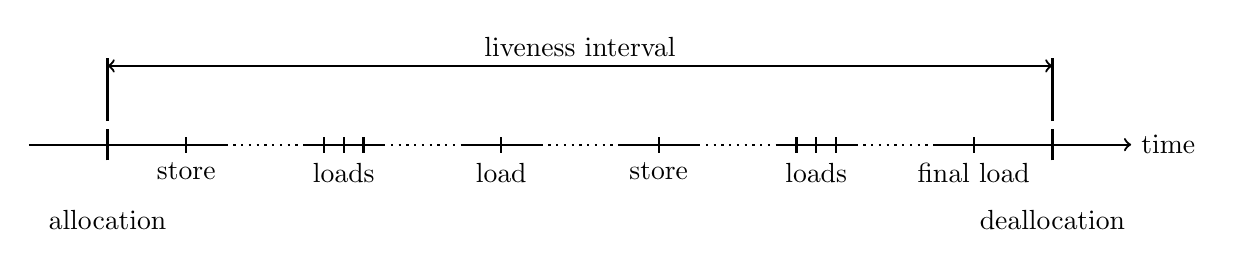
\begin{tikzpicture}
% The timeline
\draw [-][thick] (-1,0) -- (1.5,0);
\draw [dotted][thick] (1.5,0) -- (2.5,0);
\draw [-][thick] (2.5,0) -- (3.5,0);
\draw [dotted][thick] (3.5,0) -- (4.5,0);
\draw [-][thick] (4.5,0) -- (5.5,0);

\draw [dotted][thick] (5.5,0) -- (6.5,0);

\draw [-][thick] (6.5,0) -- (7.5,0);
\draw [dotted][thick] (7.5,0) -- (8.5,0);
\draw [-][thick] (8.5,0) -- (9.5,0);
\draw [dotted][thick] (9.5,0) -- (10.5,0);
\draw [->][thick] (10.5,0) -- (13,0) node[right]{time};

% Access ticks
\draw [-][thick] (0,-0.2) node[below=0.5]{allocation} -- (0,0.2);

\draw [-][thick] (1,-0.1) node[below]{store} -- (1,0.1);
\draw [-][thick] (3,-0.1) node[below]{loads} -- (3,0.1);
\draw [-][thick] (5,-0.1) node[below]{load} -- (5,0.1);
\draw [-][thick] (2.75,-0.1) -- (2.75,0.1);
\draw [-][thick] (3.25,-0.1) -- (3.25,0.1);

\draw [-][thick] (7,-0.1) node[below]{store} -- (7,0.1);
\draw [-][thick] (9,-0.1) node[below]{loads} -- (9,0.1);
\draw [-][thick] (11,-0.1) node[below]{final load} -- (11,0.1);
\draw [-][thick] (8.75,-0.1) -- (8.75,0.1);
\draw [-][thick] (9.25,-0.1) -- (9.25,0.1);

\draw [-][thick] (12,-0.2) node[below=0.5]{deallocation} -- (12,0.2);

% Liveness interval 1
\draw [-][thick] (0, 0.3) -- (0,1.1);
\draw [<->][thick] (0,1) -- (12,1);
\draw [-][thick] (12, 0.3) -- (12,1.1);
\node [above] at (6,1) {liveness interval};

\end{tikzpicture}

  \caption{Classical liveness}
  \label{fig:liveness-classical}
\end{figure}

\begin{figure}[!ht]
  \centering
  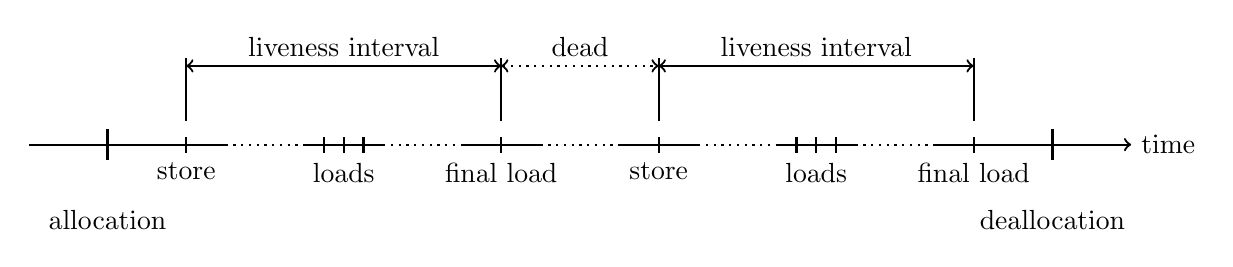
\begin{tikzpicture}
% The timeline
\draw [-][thick] (-1,0) -- (1.5,0);
\draw [dotted][thick] (1.5,0) -- (2.5,0);
\draw [-][thick] (2.5,0) -- (3.5,0);
\draw [dotted][thick] (3.5,0) -- (4.5,0);
\draw [-][thick] (4.5,0) -- (5.5,0);

\draw [dotted][thick] (5.5,0) -- (6.5,0);

\draw [-][thick] (6.5,0) -- (7.5,0);
\draw [dotted][thick] (7.5,0) -- (8.5,0);
\draw [-][thick] (8.5,0) -- (9.5,0);
\draw [dotted][thick] (9.5,0) -- (10.5,0);
\draw [->][thick] (10.5,0) -- (13,0) node[right]{time};

% Access ticks
\draw [-][thick] (0,-0.2) node[below=0.5]{allocation} -- (0,0.2);

\draw [-][thick] (1,-0.1) node[below]{store} -- (1,0.1);
\draw [-][thick] (3,-0.1) node[below]{loads} -- (3,0.1);
\draw [-][thick] (5,-0.1) node[below]{final load} -- (5,0.1);
\draw [-][thick] (2.75,-0.1) -- (2.75,0.1);
\draw [-][thick] (3.25,-0.1) -- (3.25,0.1);

\draw [-][thick] (7,-0.1) node[below]{store} -- (7,0.1);
\draw [-][thick] (9,-0.1) node[below]{loads} -- (9,0.1);
\draw [-][thick] (11,-0.1) node[below]{final load} -- (11,0.1);
\draw [-][thick] (8.75,-0.1) -- (8.75,0.1);
\draw [-][thick] (9.25,-0.1) -- (9.25,0.1);

\draw [-][thick] (12,-0.2) node[below=0.5]{deallocation} -- (12,0.2);

% Liveness interval 1
\draw [-][thick] (1, 0.3) -- (1,1.1);
\draw [<->][thick] (1,1) -- (5,1);
\draw [-][thick] (5, 0.3) -- (5,1.1);
\node [above] at (3,1) {liveness interval};

% Dead interval
\draw [-][thick] (5, 0.3) -- (5,1.1);
\draw [<->][thick, dotted] (5,1) -- (7,1);
\draw [-][thick] (7, 0.3) -- (7,1.1);
\node [above] at (6,1) {dead};

% Liveness interval 2
\draw [-][thick] (7, 0.3) -- (7,1.1);
\draw [<->][thick] (7,1) -- (11,1);
\draw [-][thick] (11, 0.3) -- (11,1.1);
\node [above] at (9,1) {liveness interval};

\end{tikzpicture}

  \caption{Liveness intervals}
  \label{fig:liveness-intervals}
\end{figure}

\Cref{fig:liveness-intervals-example} illustrates the liveness intervals of the C code example presented by \Cref{fig:mat-example-c-code}. The figure shows on the left hand-side the instruction number. On the right hand-side the instruction itself is shown. On top of the figure the addresses used by the program are listed. The core of the figure are the liveness intervals of the addresses. Each line represents a single liveness interval. A liveness interval begins at the lower instruction number and ends at the higher one. The liveness intervals are quite obvious for the addresses \texttt{\&x}, \texttt{\&y}, and \texttt{\&z}, respectively. According to Definition \ref{def:liveness-interval} a liveness interval always begins with a store instruction. Taking a look the instructions 2, 3, and 7 these indicate the beginnings of the liveness intervals for the three addresses \texttt{\&x}, \texttt{\&y}, and \texttt{\&z}. The ends of all three are indicated by load instructions at the instruction number 5, 9, and 12. Non of the addresses is access after these lines again, e.g., \texttt{\&x} not used anymore after instruction number 5. However, these are quite strait cases. The address \texttt{\&sum} presents a much more interesting case. \texttt{\&sum} consists of four liveness intervals. The first one begins at instruction number 1. This is when \texttt{\&sum} is initialized. Afterwards follow the initializations of \texttt{\&x} and \texttt{\&y} before \texttt{\&sum} is accessed again. The load at instruction number 4 indicates the end of \texttt{\&sum}s first liveness interval, because the next access at instruction number 6 is a store. This is when the second liveness interval begins. The other liveness intervals follow the same pattern. Note that even the store at instruction number 13 yields a liveness interval, even if it is the shortest possible. At the instruction number 5, 9, and 12 the address \texttt{\&sum} is \emph{dead} according to the applied definition of liveness intervals, see \Cref{fig:liveness-intervals}. It would allow to reuse the address of \texttt{\&sum} for other purposes.

\begin{figure}[!ht]
  \centering
  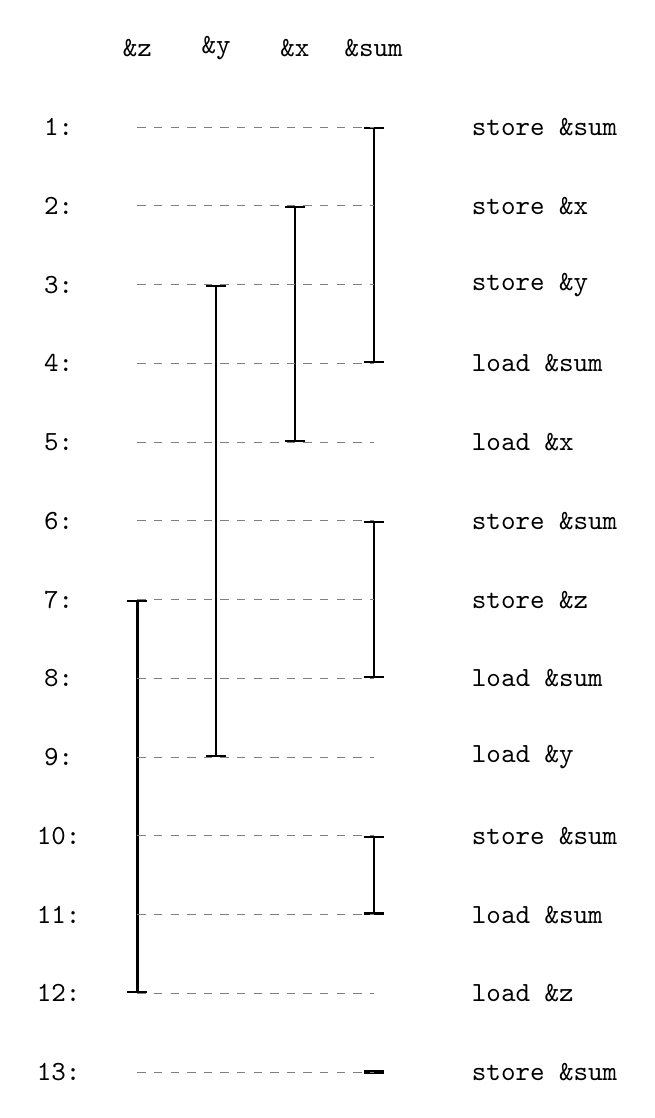
\begin{tikzpicture}

\node [align=left] at (0,0) {\texttt{\&sum}};
\node [align=left] at (-1,0) {\texttt{\&x}};
\node [align=left] at (-2,0) {\texttt{\&y}};
\node [align=left] at (-3,0) {\texttt{\&z}};

\draw [|-|][thick] (0,-1) -- (0,-4);
\draw [|-|][thick] (0,-6) -- (0,-8);
\draw [|-|][thick] (0,-10) -- (0,-11);
\draw [|-|][thick] (0,-13) -- (0,-13);
\draw [|-|][thick] (-1,-2) -- (-1,-5);
\draw [|-|][thick] (-2,-3) -- (-2,-9);
\draw [|-|][thick] (-3,-7) -- (-3,-12);

\node [label=right:\texttt{store \&sum}] at (1,-1)  {};
\node [label=right:\texttt{store \&x  }] at (1,-2)  {};
\node [label=right:\texttt{store \&y  }] at (1,-3)  {};
\node [label=right:\texttt{load  \&sum}] at (1,-4)  {};
\node [label=right:\texttt{load  \&x  }] at (1,-5)  {};
\node [label=right:\texttt{store \&sum}] at (1,-6)  {};
\node [label=right:\texttt{store \&z  }] at (1,-7)  {};
\node [label=right:\texttt{load  \&sum}] at (1,-8)  {};
\node [label=right:\texttt{load  \&y  }] at (1,-9)  {};
\node [label=right:\texttt{store \&sum}] at (1,-10) {};
\node [label=right:\texttt{load  \&sum}] at (1,-11) {};
\node [label=right:\texttt{load  \&z  }] at (1,-12) {};
\node [label=right:\texttt{store \&sum}] at (1,-13) {};

\foreach \y in {1,2,3,...,13}
{
  \node at (-4, -\y) {\texttt{\y:}};
  \draw [-][draw=gray,dashed] (-3, -\y) -- (0, -\y);
}
\end{tikzpicture}

  \caption{Liveness intervals of the C code example shown in \Cref{fig:mat-example-c-code}.}
  \label{fig:liveness-intervals-example}
\end{figure}

This section presented the definition of liveness and especially of liveness intervals. The definition of liveness intervals is one of the most central components of this work. It is the base for the trace transformations described in \Cref{sec:trace-transformation}.

%%%%%%%%%%%%%%%%%%%%%%%%%%%%%%%%%%%%%%%%%%%%%%%%%%%%%%%%%%%%%%%%%%%%%%%%%%%%%%%%%%%%%%%%%%%%%%%%%%%
% Performance
%%%%%%%%%%%%%%%%%%%%%%%%%%%%%%%%%%%%%%%%%%%%%%%%%%%%%%%%%%%%%%%%%%%%%%%%%%%%%%%%%%%%%%%%%%%%%%%%%%%

\section{Performance}\label{sec:performance}

This section presents how the performance of a trace is computed. The performance of a trace is the most significant criteria of its quality. In general \ac{trace}s with better performance use the memory available in a more efficient way than others. The performance is independent of the number of instructions a case consists of. The only important criteria are the number of memory accesses. As \Cref{fig:hardware-model} shows there are different kinds of memory accesses. Depending if the accessed address is in the cache or not the time required to load the value of a address into a register varies. Cached data can be access much faster than data which has to be loaded from main memory. The \emph{latency} to load data into a register is measured in \emph{\ac{CPU} cycles}. \ac{CPU} cycles are a common metric to measure durations at hardware level.

In our system \emph{performance} is measured in \ac{CPA}. Indeed performance is not directly measured. As \Cref{equ:performance-cpa} illustrates it is computed according to the measured number of memory accesses. \ac{CPA} describes the average number of \ac{CPU} cycles per memory access with memory access equivalent to an instruction of the trace.

We proceed as follows, after the \ac{trace} of a program has been generated its performance is analyzed by applying the trace on a simulated cache model and counting the different kinds of memory accesses. At the end of the execution the performance is computed as illustrated by \Cref{equ:performance-cpa}.

\begin{equation}\label{equ:performance-cpa}
\text{CPA}(T,C) = \frac{\text{Sum of cycles}(T, C)}{\text{Sum of accesses}(T)}
\end{equation}

$T$ represents the \ac{trace} of the analyzed program. $C$ represents the applied cache model, the different cache models are explained in \Cref{sec:cache-models}.

\emph{sum of cycles(T, C)} represents the sum of all memory accesses each weight according to its costs. The costs for a memory access the depends on the latency of the memory unit accessed. This is why cache accesses are cheaper than main memory accesses. The \emph{sum of accesses(T)} represents the total number of load and store instructions executed by the \ac{trace} $T$.

\Cref{tab:memory-access-cost} shows the costs for the different types of memory accesses. These numbers are taken form literature \cite{drepper2007every}, \cite{skylake}. The actual values are not that important than the relation of cache instruction costs to the memory instruction costs.

\begin{table}[!ht]
  \centering
  \begin{tabular}{lc}
  \hline
  Memory Access Type & Cost in Cycles \\
  \hline
  Cache  load  & 1 \\
  Cache  store & 1 \\
  Memory load  & 5 \\
  Memory store & 5 \\
  \hline
  \end{tabular}
  \caption{Cost for memory access types}
  \label{tab:memory-access-cost}
\end{table}

This section presents our definition of performance and how the performance of a trace is computed. For this procedure the memory accesses of a  \ac{trace} are recored and finally used for computation. The performance is the average number of \ac{CPU} cycles per \ac{trace} instruction.

%%%%%%%%%%%%%%%%%%%%%%%%%%%%%%%%%%%%%%%%%%%%%%%%%%%%%%%%%%%%%%%%%%%%%%%%%%%%%%%%%%%%%%%%%%%%%%%%%%%
% Metrics
%%%%%%%%%%%%%%%%%%%%%%%%%%%%%%%%%%%%%%%%%%%%%%%%%%%%%%%%%%%%%%%%%%%%%%%%%%%%%%%%%%%%%%%%%%%%%%%%%%%

\section{Metrics}\label{sec:metrics}

This section presents the metrics chosen to characterize a \ac{trace}. The characteristic of \ac{trace} consists of the four metrics \emph{accesses}, \emph{access distance}, \emph{overlapping liveness}, and \emph{liveness interval length}. These are used to reason about the resulting performance of a \ac{trace} and further to compare a \ac{trace} with other \ac{trace}s. The metrics presented by this section are all applied after \ac{trace} transformation. So, these operated on variables rather than directly on addresses. Nevertheless, variables could easily be mapped to addresses. Furthermore, for all four metrics the same statistical parameters are computed: minimum, maximum, average, 5\% percentile, 25\% percentile, 50\% percentile, 75\% percentile, and 95\% percentile.

\begin{remark} Statical metrics\
\begin{itemize}
\item The \emph{minimum} is the numerical smallest value of all samples.
\item The \emph{maximum} is the numerical largest value of all samples.
\item The \emph{average} is the arithmetic mean of all samples. It is computed by dividing the sum of all samples by the number of samples.
\item The \emph{percentile} is the value below which a given percentage of samples of all samples fall, i.e., the 25\% percentile represents the value for which holds that 25\% of all samples are smaller than this value. The $k$th percentile is computed by sorting all samples from smallest to largest. Multiply the $k$ percent by the total number of values, this is the index within the sorted list of samples. The $k$ percentile is the value at the computed index.
\end{itemize}
\end{remark}

\begin{figure}[!ht]
  \centering
  \begin{tabular}{c}
  \begin{lstlisting}
1: load  A
2: load  B
3: store A
  \end{lstlisting}
  \end{tabular}
  \caption{Tiny \ac{trace} example. Note: this trace has been transformed, i.e., there is no \texttt{\&} so \texttt{A} and \texttt{B} represent variables not addresses. On the left the instruction number is shown and on the right the correlating instruction is presented.}
  \label{fig:metrics-exmaple}
\end{figure}

\subsection{Accesses}\label{ssec:metric-accesses}
The metric called \emph{accesses} is as simple as the name suggests. It investigates on the number of accesses on a certain variable. For this reason the number of accesses on each variable are counted. Independent of an access is a load or store each counts the same. In other words this metric shows how often a variables occurs within a \ac{trace}. Finally, the statistical metrics as explained above are computed on the observed sample. Applying this metric on the tiny example presented by \Cref{fig:metrics-exmaple} results in following list of samples $(1, 2)$. Variable $A$ is accessed twice and variable $B$ is accessed only once.

\subsection{Access Distance}\label{ssec:metric-access-distance}
The \emph{access distance} metric shows the distance between two sequential accesses on the same variable, e.g, if there is only one variable accessed the access distance of such a \ac{trace} is 0, but assume a \ac{trace} which accesses two variables alternating as shown by \Cref{fig:metrics-access-distance-exmaple} then the access distance of $A$ is 2. Its computed by subtracting the instruction number of the last access by the current instruction number, i.e., in case of $A$ the access distance is computed by $3-1 = 2$, same of $B$ ($2 - 2 = 0$). Finally, the statistical metrics as explained above are computed on the observed sample. Applying this metric on the tiny example presented by \Cref{fig:metrics-exmaple} results in following list of samples $(0, 2)$. Between the load of variable $A$ and the store on it there is only one other instruction this is why there is a $1$ in the list. The $0$ results for variable $B$ which accessed only once.

\subsection{Overlapping Liveness}\label{ssec:metric-concurrently-live}
The \emph{overlapping liveness} metric presents the number of variables which are live at a certain instruction number, i.e., this metric is equivalent with the number of overlapping liveness intervals observed for each instruction number. The set of live variable which are currently used is called \emph{working set}. The term working set has been introduced by the work \cite{denning1968working}. This metric shows how a \ac{trace}s working set size behaves. For this reason at each instruction the currently live variables are counted. The observed value is appended to then set of samples. Finally, the statistical metrics as explained above are computed on the observed sample. Applying this metric on the tiny example presented by \Cref{fig:metrics-exmaple} results in following list of samples $(1, 1, 2)$. At instruction number 1 and 3 only one variable is live $A$, namely. At instruction number 2 there are two variables live $A$, and $B$, respectively.

\subsection{Liveness Interval Length}\label{ssec:metric-liveness-interval-length}
The \emph{liveness interval length} metric illustrates the different lengths of liveness intervals. Variables are used for a certain timespan and this timespan varies. In general there are variables which are used for a short period and others are live for longer. If a variable is only accessed once the liveness interval length is $0$. The liveness interval length is computed similar to the access distance by subtracting the instruction number of beginning of a liveness interval from the instruction number of its last access. Finally, the statistical metrics as explained above are computed on the observed sample. Applying this metric on the tiny example presented by \Cref{fig:metrics-exmaple} results in following list of samples $(0, 2)$. As explained above if a variable is only accessed once the liveness interval length is $0$, this is the case of $B$. The length of the liveness interval of variable $A$ is represented by the second value of the list, $2$.

%%%%%%%%%%%%%%%%%%%%%%%%%%%%%%%%%%%%%%%%%%%%%%%%%%%%%%%%%%%%%%%%%%%%%%%%%%%%%%%%%%%%%%%%%%%%%%%%%%%
% Trace Transformation
%%%%%%%%%%%%%%%%%%%%%%%%%%%%%%%%%%%%%%%%%%%%%%%%%%%%%%%%%%%%%%%%%%%%%%%%%%%%%%%%%%%%%%%%%%%%%%%%%%%

\section{Trace Transformation}\label{sec:trace-transformation}

\Cref{sec:memory-access-trace} illustrated how to observe the \ac{trace} of a program. \Cref{sec:liveness} describes our definition of liveness and introduces liveness intervals. This section shows how to use these information to transform the \ac{trace} $T$ of a program. The aim is to transform a \ac{trace} $T$ into a \ac{trace} $T'$ which is semantically equivalent to $T$ but which offers better performance. The performance of a \ac{trace} is judged as shown in \Cref{sec:performance}. During transformation the addresses of the original \ac{trace} are replaced by other addresses.

We distinguish the originally used addresses form the addresses used after transformation. The latter ones are called \emph{variables}. A \emph{variable} is in general nothing else than an address. There are two significant reasons why to use a different naming.

First the original addresses have some properties like being an address on the heap or being an address of the globals or being an address within the program code which introduces some restrictions. For our purpose this information is not important. During transformation we do not care about this. Each address is handled the same way.

Second it simplifies talking about \ac{trace}s. Each time we talk about an address it refers to the \ac{trace} observed form the binary. Talking about variables indicates that the \ac{trace} has been transformed already.

\subsection{Identity Trace}

For transformation simply the addresses of a \ac{trace} are replaces by variables. There are no further changes. Based on the \ac{trace} (see \Cref{fig:mat-example-trace}) observed from the C code illustrates by \Cref{fig:mat-example-c-code} the addresses are replaces by variables as shown by \Cref{fig:trace-transformation-original}. Basically, \texttt{\&sum} becomes $A$, \texttt{\&x} becomes $B$, \texttt{\&y} becomes $C$, and \texttt{\&z} becomes $D$. Obviously, there is one more difference the x-axis and y-axis are switched, namely. The reason is simple because it requires less space vertically. However, note that liveness intervals of the variables shown by \Cref{fig:trace-transformation-original} are exactly the same as those of the addresses illustrated by \Cref{fig:liveness-intervals-example}.

\begin{figure}[!ht]
  \centering
  \begin{tikzpicture}

\node [align=left] at (0,0) {A};
\draw [|-|][thick] (1,0) -- (4,0);
\draw [|-|][thick] (6,0) -- (8,0);
\draw [|-|][thick] (10,0) -- (11,0);
\draw [|-|][thick] (13,0) -- (13,0);

\node [align=left] at (0,-1) {B};
\draw [|-|][thick] (2,-1) -- (5,-1);

\node [align=left] at (0,-2) {C};
\draw [|-|][thick] (3,-2) -- (9,-2);

\node [align=left] at (0,-3) {D};
\draw [|-|][thick] (7,-3) -- (12,-3);

\foreach \x in {1,2,3,...,13}
{
	\node at (\x,-7) {\x};
	\draw [-][draw=gray,dashed] (\x,-6.5) -- (\x,0.5);
}
\end{tikzpicture}

  \caption{Liveness intervals of the C code example shown in \Cref{fig:mat-example-c-code}.}
  \label{fig:trace-transformation-original}
\end{figure}

In this work two different kinds of \ac{trace} transformations are applied, expanding the \ac{trace} and collapsing the \ac{trace}.

\subsection{Single Assignment Trace}

For expanding a \ac{trace} we decided to use a \emph{single assignment} form. More concrete each liveness interval of a \ac{trace} is assigned to its own variable. Further, a variable is never assigned a liveness interval more often than exactly once. \Cref{fig:trace-transformation-sa} presents the \emph{single assignment trace} of \Cref{fig:mat-example-trace}. It is not surprising that the number of variable required increases applying this approach. In detail the four liveness intervals of address \texttt{\&sum} are know assigned to the variables $A$, $D$, $F$, and $G$. The variable a liveness interval is assigned to depends on its beginning. This is why the variables used to map the liveness intervals of address \texttt{\&sum} are not contiguous. For this approach walk through the \ac{trace} and each time a store instruction occurs assign the next free variable, e.g., in alphabetical order as shown by the example. The implementation details are explained in \Cref{ssec:allocator-single-assignment}.

\begin{figure}[!ht]
  \centering
  \begin{tikzpicture}

\node [align=left] at (0,0) {A};
\draw [|-|][thick] (1,0) -- (4,0);

\node [align=left] at (0,-1) {B};
\draw [|-|][thick] (2,-1) -- (5,-1);

\node [align=left] at (0,-2) {C};
\draw [|-|][thick] (3,-2) -- (9,-2);

\node [align=left] at (0,-3) {D};
\draw [|-|][thick] (6,-3) -- (8,-3);

\node [align=left] at (0,-4) {E};
\draw [|-|][thick] (7,-4) -- (12,-4);

\node [align=left] at (0,-5) {F};
\draw [|-|][thick] (10,-5) -- (11,-5);

\node [align=left] at (0,-6) {G};
\draw [|-|][thick] (13,-6) -- (13,-6);

\foreach \x in {1,2,3,...,13}
{
  \node at (\x,-7) {\x};
  \draw [-][draw=gray,dashed] (\x,-6.5) -- (\x,0.5);
}
\end{tikzpicture}

  \caption{Liveness intervals of the C code example shown in \Cref{fig:mat-example-c-code} in \emph{single assignment} form.}
  \label{fig:trace-transformation-sa}
\end{figure}

\subsection{Compact Trace}

For collapsing a \ac{trace} we to use a \emph{compact} form. More concrete each liveness interval of a \ac{trace} is assigned to a variable, but now variables are \emph{reused}. If the liveness interval ends the variable is added to a \emph{free list}, i.e., a list of variable already use before but there liveness intervals already ended. The procedure is as follows before using a new variable the free list is checked. If there are variables available at the free list these are used. Otherwise an new variable is assigned. The implementation details are explained in \Cref{ssec:allocator-compact}. There are various ways opportunities for the semantics of the free list. In this work three variants are investigated, (1) stack semantic presented by \Cref{sssec:allocator-compact-stack}, (2) queue semantic explained by \Cref{sssec:allocator-compact-queue}, and (3) set semantic shown by \Cref{sssec:allocator-compact-set}. The set semantic is thought to represent a random selection of a free variable. However, \Cref{fig:trace-transformation-compact} illustrates the compaction of the \ac{trace} shown in \Cref{fig:mat-example-trace} and applies a free list with stack semantics. As expected this approach requires less variables. The liveness intervals of \texttt{\&sum} remain the the same variable $A$. Furthermore, the addresses \texttt{\&x} and \texttt{\&z} now share variable $B$.

\begin{remark}
Note that only by coexistent the liveness intervals of address \texttt{\&sum} are assigned to the same variable $A$. In general is depends on the semantics of the free list and the currently free variables which variable a liveness interval is assigned to.
\end{remark}

\begin{figure}[!ht]
  \centering
  \begin{tikzpicture}

\node[align=left] at (0,0) {A};
\draw [|-|][thick] (1,0) -- (4,0);
\draw [|-|][thick] (6,0) -- (8,0);
\draw [|-|][thick] (10,0) -- (11,0);
\draw [|-|][thick] (13,0) -- (13,0);

\node [align=left] at (0,-1) {B};
\draw [|-|][thick] (2,-1) -- (5,-1);
\draw [|-|][thick] (7,-1) -- (12,-1);

\node [align=left] at (0,-2) {C};
\draw [|-|][thick] (3,-2) -- (9,-2);

\foreach \x in {1,2,3,...,13}
{
  \node at (\x,-7) {\x};
  \draw [-][draw=gray,dashed] (\x,-6.5) -- (\x,0.5);
}
\end{tikzpicture}

  \caption{Liveness intervals of the C code example shown in \Cref{fig:mat-example-c-code} in \emph{compacted} form.}
  \label{fig:trace-transformation-compact}
\end{figure}

This section presents two different kinds of \ac{trace} transformations, single assignment and compaction, namely. Single assignment potentially increases the number of used variables and compaction potentially decreases the number of used variables.

%%%%%%%%%%%%%%%%%%%%%%%%%%%%%%%%%%%%%%%%%%%%%%%%%%%%%%%%%%%%%%%%%%%%%%%%%%%%%%%%%%%%%%%%%%%%%%%%%%%
% Summarizing Example
%%%%%%%%%%%%%%%%%%%%%%%%%%%%%%%%%%%%%%%%%%%%%%%%%%%%%%%%%%%%%%%%%%%%%%%%%%%%%%%%%%%%%%%%%%%%%%%%%%%

\section{Summarizing Example}

Lets take a look at the performance of the three \ac{trace}s from above. Assume a \ac{LRU} cache with 2 cache lines, each cache line fits exactly one variable. For details on \ac{LRU} caches see \Cref{ssec:cache-lru}. As a breath description of the applied cache model imaging as long as there is a free cache line within the cache this one is used. In case of an eviction, there is no more free space in the cache, the \emph{least recently used} cache line is evicted to make space for a new one.

If a variable is accessed which is already in the cache a cheap cache access can be executed, either a load or store instruction. Otherwise, a much more expensive main memory instruction has to be executed. The costs of these instructions are presented by \Cref{tab:memory-access-cost}. For the following performance computation we assume a simple optimization. The first store instruction on a variable can be executed directly into the cache. Furthermore, assume that in case of an eviction the data of a variable is stored in main memory. Independent, if the variable is still alive or already dead.

\subsection{Identity Trace}
\Cref{fig:trace-transformation-original-marked} shows the annotated liveness intervals of the identity \ac{trace} of \Cref{fig:trace-transformation-original}. According to the assumptions from above every beginning of a liveness interval is annotated with a cache store instruction. Since the assumed cache model fits exactly two variables the first eviction occurs when writing variable $C$ at instruction 3. According to the eviction policy of the applied \ac{LRU} cache variable $A$ is evicted. The memory store of variable $A$ is annotated with a filled red circle. Unfortunately, variable $A$ is accessed at the next instruction. For this reason it has to be loaded from main memory again, but before $B$ is stored in main memory to make space in the cache for $A$. The same procedure repeats for the variables $B$ and $C$ at instruction number 5. At instruction number 6 we are able to load a variable directly from cache for the first time. Nevertheless, there are two more eviction required to finish the execution of this trace. One at instruction 7, variable $B$ is evicted to make space for variable $D$ which is accessed for the first time. A interesting aspect at this instruction is that the liveness interval of variable $B$ end two instruction before, so $B$ is dead. Furthermore, $B$ is not needed anymore for the following instructions. In general this information is not available, this is why there is a memory store annotated. But if a systems knows about the liveness intervals of its variables it might decide to overwrite the value of $B$ by the value of $D$ and avoid the memory store. The last eviction appears at instruction 9 when variable $C$ is accessed for the last time. Variable $A$ is accessed several time without any interaction with the main memory, because each time it is access it is in the cache.

\begin{figure}[!ht]
  \centering
  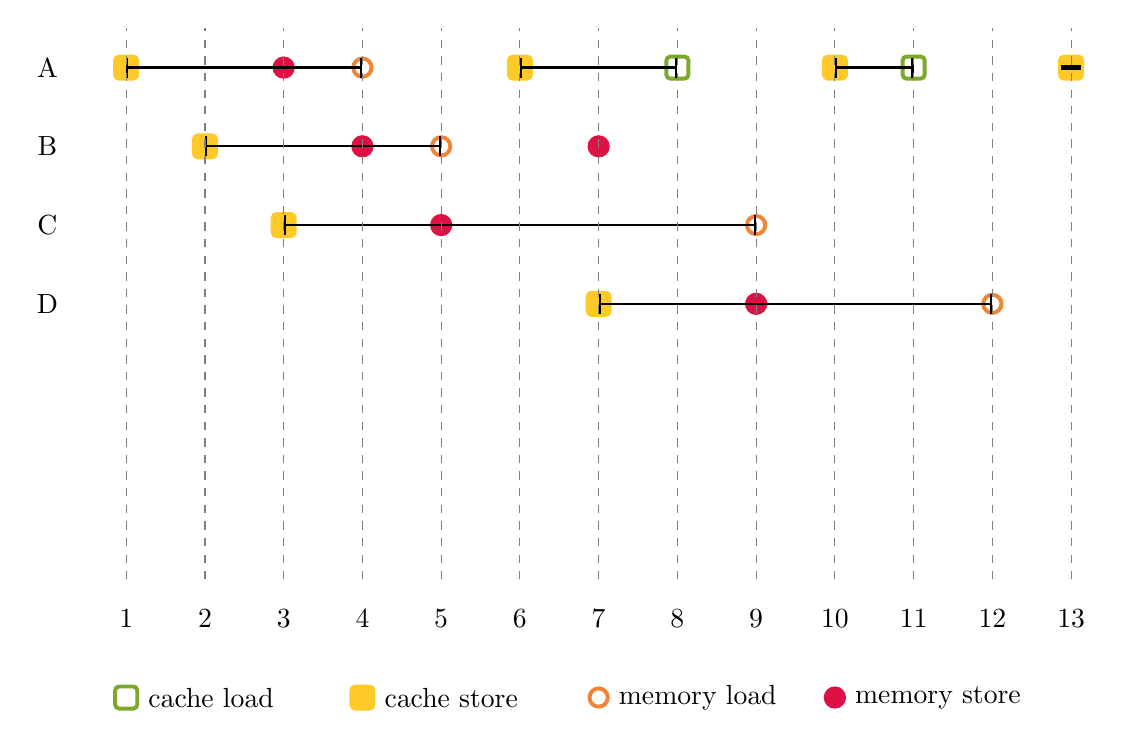
\begin{tikzpicture}

\node [align=left] at (0,0) {A};
\node[cache-store] at (1,0) {};
\node[memory-store] at (3,0) {};
\node[memory-load] at (4,0) {};
\node[cache-store] at (6,0) {};
\node[cache-load] at (8,0) {};
\node[cache-store] at (10,0) {};
\node[cache-load] at (11,0) {};
\node[cache-store] at (13,0) {};
\draw [|-|][thick] (1,0) -- (4,0);
\draw [|-|][thick] (6,0) -- (8,0);
\draw [|-|][thick] (10,0) -- (11,0);
\draw [|-|][thick] (13,0) -- (13,0);

\node [align=left] at (0,-1) {B};
\node[cache-store] at (2,-1) {};
\node[memory-store] at (4,-1) {};
\node[memory-load] at (5,-1) {};
\node[memory-store] at (7,-1) {};
\draw [|-|][thick] (2,-1) -- (5,-1);

\node [align=left] at (0,-2) {C};
\node[cache-store] at (3,-2) {};
\node[memory-store] at (5,-2) {};
\node[memory-load] at (9,-2) {};
\draw [|-|][thick] (3,-2) -- (9,-2);

\node [align=left] at (0,-3) {D};
\node[cache-store] at (7,-3) {};
\node[memory-store] at (9,-3) {};
\node[memory-load] at (12,-3) {};
\draw [|-|][thick] (7,-3) -- (12,-3);

\node[cache-load,   label=right:cache load]   at  (1,-8) {};
\node[cache-store,  label=right:cache store]  at  (4,-8) {};
\node[memory-load,  label=right:memory load]  at  (7,-8) {};
\node[memory-store, label=right:memory store] at (10,-8) {};

\foreach \x in {1,2,3,...,13}
{
	\node at (\x,-7) {\x};
	\draw [-][draw=gray,dashed] (\x,-6.5) -- (\x,0.5);
}
\end{tikzpicture}

  \caption{Liveness intervals of the C code example shown in \Cref{fig:mat-example-c-code}. Annotated by the different kinds of memory accesses. Assuming a LRU cache with 2 cache lines, each cache line fits exactly one variable.}
  \label{fig:trace-transformation-original-marked}
\end{figure}

The metrics of the \ac{trace} illustrated by \Cref{fig:trace-transformation-original-marked} characterize it. The \emph{accesses} metric is observed by counting all accesses on a certain variable. In this example the list of samples holds four values one for each variable. The number of accesses on variable $A$ is $7$, on all other variables are accessed twice. The resulting and (sorted) list of samples looks as follows $(2, 2, 2, 7)$. The \emph{access distance} presents kind of the access frequency on an variable. Depending on the number of accesses the list of access distances could be significantly larger than the number of used variables. In this case the sorted list of samples looks as follows $(0, 1, 2, 2, 2, 2, 3, 3, 5, 6)$. For variable $A$ there are multiple access distances (from left to write) $3$, $2$, $2$, $2$, $1$, and $0$, namely. The \emph{overlapping liveness} metrics shows how many variables are used at the same instruction number. The list of samples is computed by counting the overlapping liveness intervals for each instruction number. As a result the size of the samples list depends on the number of instructions rather than on the number of used variables. In case of the current example the samples are $(1, 2, 3, 3, 2, 2, 3, 3, 2, 2, 2, 1, 1)$. For the purpose of better understanding the list is on sorted instead it is ordered according to the correlating instruction number, i.e., the first entry represents the number of overlapping liveness variable at instruction number 1 and the last entry represents this value for instruction number 13. The fourth metric is the \emph{liveness interval length}. The number of used variables and the number of accesses on a variables define number of samples for this metric. The number of accesses on a variable are signification because these define the liveness intervals. For this example the list of samples looks as follows $(0, 1, 2, 3, 3, 5, 6)$. For variable $A$ there are four entry in the list $0$, $1$, $2$, and $3$. The resulting metrics are presented by \Cref{tab:summarizing-example-metrics-original}.

\begin{table}[!ht]
  \centering
  \begin{tabular}{lrrrrrrrr}
    \hline
    \multirow{2}{*}{Metric} & \multirow{2}{*}{Min.} & \multirow{2}{*}{Max.} & \multirow{2}{*}{Avg.} & \multicolumn{5}{c}{Percentile} \tabularnewline
    & & & & 5\% & 25\% & 50\% & 75\% & 95\% \tabularnewline
    \hline
    Accesses                 & 2.00 & 7.00 & 3.25 & 2.00 & 2.00 & 2.00 & 3.25 & 6.25 \\
    Access Distance          & 0.00 & 6.00 & 2.60 & 0.45 & 2.00 & 2.00 & 3.00 & 5.55 \\
    Overlapping Liveness        & 1.00 & 3.00 & 2.08 & 1.00 & 2.00 & 2.00 & 3.00 & 3.00 \\
    Liveness Interval Length & 0.00 & 6.00 & 2.86 & 0.30 & 1.50 & 3.00 & 4.00 & 5.69 \\
    \hline
  \end{tabular}
  \caption{Metrics of the identity \ac{trace} illustrated by \Cref{fig:trace-transformation-original-marked} (values are rounded).}
  \label{tab:summarizing-example-metrics-original}
\end{table}

To compute the performance of \Cref{equ:trace-transformation-original-marked} the different kinds of memory access have to be counted and weight as illustrated by \Cref{equ:trace-transformation-original-marked}. According to the annotations of \Cref{fig:trace-transformation-original-marked} there are 2 cache load, 7 cache stores, 4 memory loads, and 5 memory stores. The result of this equation indicates that 4.15 \ac{CPU} cycles are required in average to proceed one instruction of the \ac{trace}.

\begin{equation}\label{equ:trace-transformation-original-marked}
\text{\ac{CPA}}(T_{original}, C_{LRU}) = \frac{1 * (2 + 7) + 5 * (4 + 5)}{13} = 4.15
\end{equation}

\subsection{Single Assignment Trace}
\Cref{fig:trace-transformation-sa-marked} shows the annotated liveness intervals of the single assignment trace of \Cref{fig:trace-transformation-sa}. Unexpectedly, the number of cache stores increases according to the number of variables used. On the one hand the assumption of executing the first store on a variable directly on the cache and using more variables result in more cache store instructions. On the other hand by using more addresses the number of cache loads seams to reduce for this example. In total the number of cache instructions is the same as required for the identity \ac{trace}, but the distribution is a different. Taking a look at the main memory accesses we observe an increased number of memory stores. The number of memory loads is the same. The more variables used the more variables have to be saved in main memory in case of eviction. Compared to \Cref{fig:trace-transformation-original} there three times more memory stores on variables which are already dead. The other four memory store instructions executed are identical to those of the identity \ac{trace}.

\begin{figure}
  \centering
  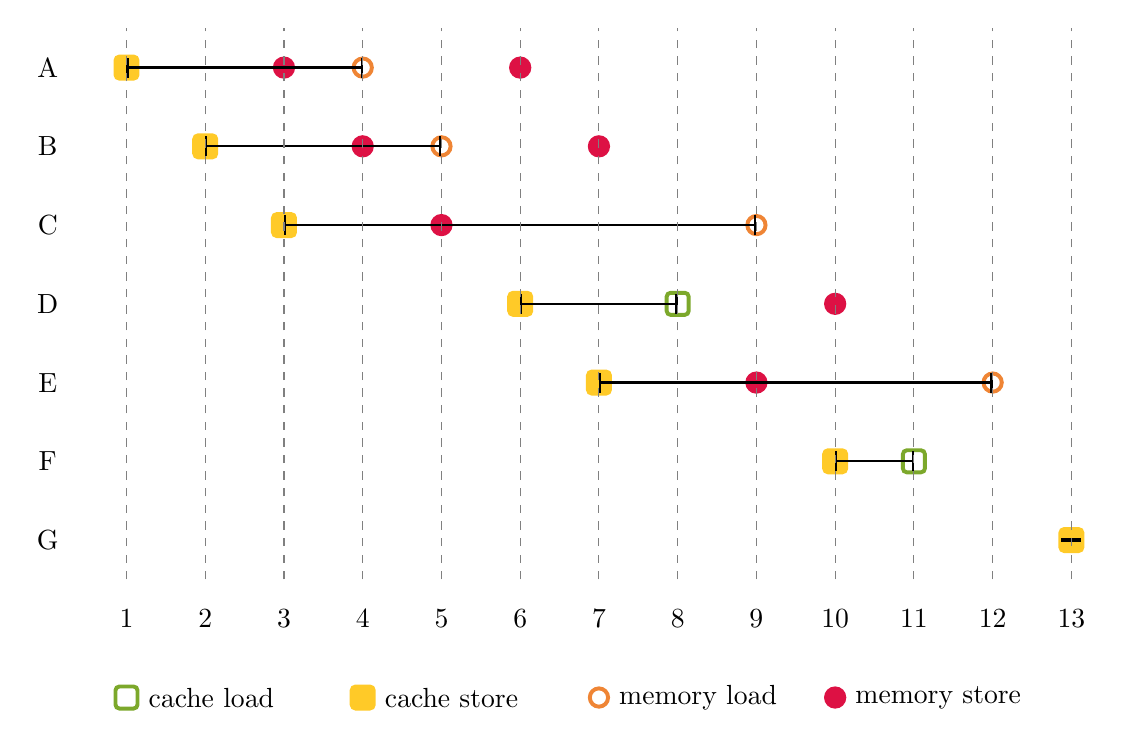
\begin{tikzpicture}

\node [align=left] at (0,0) {A};
\node[cache-store] at (1,0) {};
\node[memory-store] at (3,0) {};
\node[memory-load] at (4,0) {};
\node[memory-store] at (6,0) {};
\draw [|-|][thick] (1,0) -- (4,0);

\node [align=left] at (0,-1) {B};
\node[cache-store] at (2,-1) {};
\node[memory-store] at (4,-1) {};
\node[memory-load] at (5,-1) {};
\node[memory-store] at (7,-1) {};
\draw [|-|][thick] (2,-1) -- (5,-1);

\node [align=left] at (0,-2) {C};
\node[cache-store] at (3,-2) {};
\node[memory-store] at (5,-2) {};
\node[memory-load] at (9,-2) {};
\draw [|-|][thick] (3,-2) -- (9,-2);

\node [align=left] at (0,-3) {D};
\node[cache-store] at (6,-3) {};
\node[cache-load] at (8,-3) {};
\node[memory-store] at (10,-3) {};
\draw [|-|][thick] (6,-3) -- (8,-3);

\node [align=left] at (0,-4) {E};
\node[cache-store] at (7,-4) {};
\node[memory-store] at (9,-4) {};
\node[memory-load] at (12,-4) {};
\draw [|-|][thick] (7,-4) -- (12,-4);

\node [align=left] at (0,-5) {F};
\node[cache-store] at (10,-5) {};
\node[cache-load] at (11,-5) {};
\draw [|-|][thick] (10,-5) -- (11,-5);

\node [align=left] at (0,-6) {G};
\node[cache-store] at (13,-6) {};
\draw [|-|][thick] (13,-6) -- (13,-6);

\node[cache-load,   label=right:cache load]   at  (1,-8) {};
\node[cache-store,  label=right:cache store]  at  (4,-8) {};
\node[memory-load,  label=right:memory load]  at  (7,-8) {};
\node[memory-store, label=right:memory store] at (10,-8) {};

\foreach \x in {1,2,3,...,13}
{
  \node at (\x,-7) {\x};
  \draw [-][draw=gray,dashed] (\x,-6.5) -- (\x,0.5);
}
\end{tikzpicture}

  \caption{Liveness intervals of the C code example shown in \Cref{fig:mat-example-c-code} in \emph{single assignment} form. Annotated by the different kinds of memory accesses. Assuming a LRU cache with 2 cache lines, each cache line fits exactly one variable.}
  \label{fig:trace-transformation-sa-marked}
\end{figure}

As introduces by \Cref{ssec:metric-accesses} the access distance for the \ac{trace} presented by \Cref{fig:trace-transformation-sa} is computed. The resulting list of samples looks as follows $(1, 2, 2, 2, 2, 2, 2)$. As expected for each variable there is only one entry in the list. Different to the accesses of the identity \ac{trace} there are more entries. By coincident each variable except $G$ is accessed twice. Computing the \emph{access distance} results in following list of samples $(0, 1, 2, 3, 3, 5, 6)$. The \emph{overlapping liveness} variables are observed by counting the overlapping liveness intervals and result in the displayed list $(1, 2, 3, 3, 2, 2, 3, 3, 2, 2, 2, 1, 1)$. Since the liveness intervals are not change during transforming a \ac{trace} these values are the same as for the identity \ac{trace}. The samples for the \emph{liveness interval length} look as follows $(0, 1, 2, 3, 3, 5, 6)$. For this example the samples of the access distance and the liveness interval length are identical, but this is a coincident and not generally the case. \Cref{tab:summarizing-example-metrics-sa} presents the statistical metrics.

\begin{table}[!ht]
  \centering
  \begin{tabular}{lrrrrrrrr}
    \hline
    \multirow{2}{*}{Metric} & \multirow{2}{*}{Min.} & \multirow{2}{*}{Max.} & \multirow{2}{*}{Avg.} & \multicolumn{5}{c}{Percentile} \tabularnewline
    & & & & 5\% & 25\% & 50\% & 75\% & 95\% \tabularnewline
    \hline
    Accesses                 & 1.00 & 2.00 & 1.86 & 1.30 & 2.00 & 2.00 & 2.00 & 2.00 \\
    Access Distance          & 0.00 & 6.00 & 2.86 & 0.30 & 1.50 & 3.00 & 4.00 & 5.67 \\
    Overlapping Liveness        & 1.00 & 3.00 & 2.08 & 1.00 & 2.00 & 2.00 & 3.00 & 3.00 \\
    Liveness Interval Length & 0.00 & 6.00 & 2.86 & 0.30 & 1.50 & 3.00 & 4.00 & 5.69 \\
    \hline
  \end{tabular}
  \caption{Metrics of the single assignment trace \ac{trace} illustrated by \Cref{fig:trace-transformation-sa-marked} (values are rounded).}
  \label{tab:summarizing-example-metrics-sa}
\end{table}

The performance is computed as defined above. For this single assignment trace we observe 2 cache loads, 7 cache stores, 4 memory loads, and 7 memory stores which results in a \ac{CPA} of 4.92. This result is slightly worse than the \ac{CPA} of the identity \ac{trace} presented by \Cref{equ:trace-transformation-original-marked}.

\begin{equation}\label{equ:trace-transformation-sa-marked}
\text{\ac{CPA}}(T_{single~assigment}, C_{LRU}) = \frac{1 * (2 + 7) + 5 * (4 + 7)}{13} = 4.92
\end{equation}

\subsection{Compact Trace}
\Cref{fig:trace-transformation-compact-marked} shows the annotated liveness intervals of the compact trace of \Cref{fig:trace-transformation-compact}. The most significant difference compared to the others two trace is the number of variables used. Variable $B$ is reused for the variable $D$ of the identity \ac{trace}. Obviously, there are less memory stores required than for the single assignment trace. Furthermore, there are even less memory stores required than for the identity \ac{trace}. The reason is that reusing variable $B$ turn the memory store into a cache store of the new value. The other memory accesses are quite similar as explained above. Each liveness interval begins with a cache store. Variable $A$ allows two cache loads. The memory stores on the instructions 3, 4, 5, and 9 are identical for all three traces. Same for the memory loads at instruction 4, 5, 9, and 12.

\begin{figure}
  \centering
  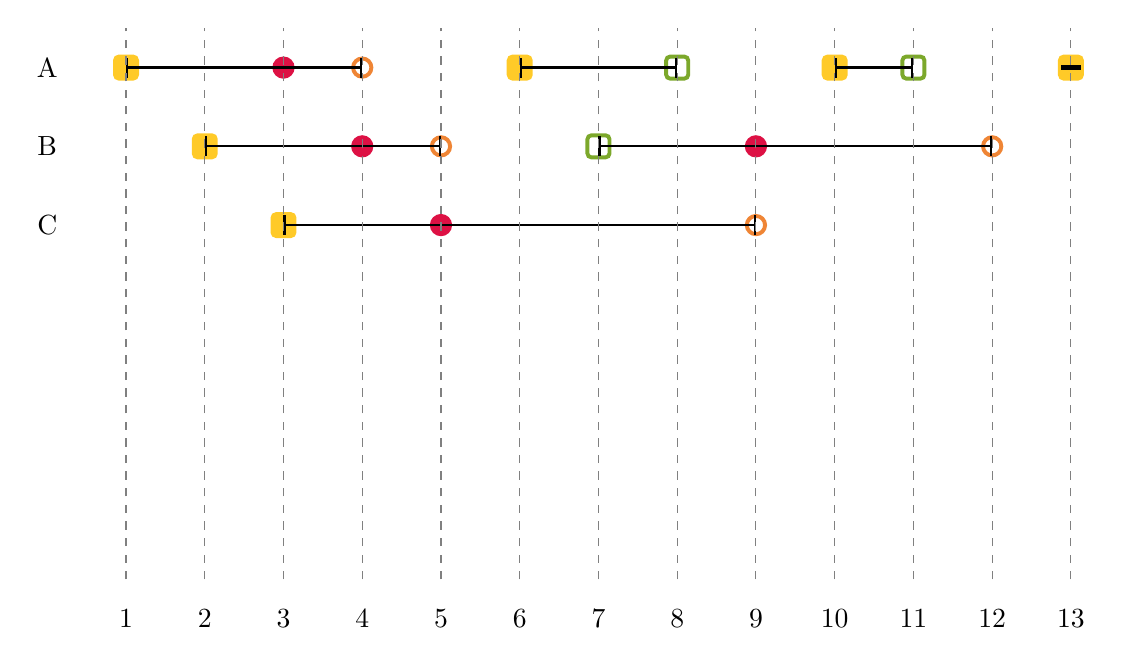
\begin{tikzpicture}

\node [align=left] at (0,0) {A};
\node[cache-store] at (1,0) {};
\node[memory-store] at (3,0) {};
\node[memory-load] at (4,0) {};
\node[cache-store] at (6,0) {};
\node[cache-load] at (8,0) {};
\node[cache-store] at (10,0) {};
\node[cache-load] at (11,0) {};
\node[cache-store] at (13,0) {};
\draw [|-|][thick] (1,0) -- (4,0);
\draw [|-|][thick] (6,0) -- (8,0);
\draw [|-|][thick] (10,0) -- (11,0);
\draw [|-|][thick] (13,0) -- (13,0);

\node [align=left] at (0,-1) {B};
\node[cache-store] at (2,-1) {};
\node[memory-store] at (4,-1) {};
\node[memory-load] at (5,-1) {};
\node[cache-load] at (7,-1) {};
\node[memory-store] at (9,-1) {};
\node[memory-load] at (12,-1) {};
\draw [|-|][thick] (2,-1) -- (5,-1);
\draw [|-|][thick] (7,-1) -- (12,-1);

\node [align=left] at (0,-2) {C};
\node[cache-store] at (3,-2) {};
\node[memory-store] at (5,-2) {};
\node[memory-load] at (9,-2) {};
\draw [|-|][thick] (3,-2) -- (9,-2);


\foreach \x in {1,2,3,...,13}
{
  \node at (\x,-7) {\x};
  \draw [-][draw=gray,dashed] (\x,-6.5) -- (\x,0.5);
}
\end{tikzpicture}

  \caption{Liveness intervals of the C code example shown in \Cref{fig:mat-example-c-code} in \emph{compacted} form. Annotated by the different kinds of memory accesses. Assuming a LRU cache with 2 cache lines, each cache line fits exactly one variable.}
  \label{fig:trace-transformation-compact-marked}
\end{figure}

For the \ac{trace} presented by \Cref{fig:trace-transformation-compact} the list of samples for th \emph{accesses} metric is $(2, 4, 7)$. According the number of used variables the list holds only three vales. The samples of the \emph{access distance} looks as follows $(0, 1, 2, 2, 2, 2, 2, 3, 3, 5, 6)$. The resulting statistical metrics are presented by \Cref{tab:summarizing-example-metrics-compact}. The \emph{overlapping liveness} metrics yields in the same list of samples as for the identity \ac{trace} and the single assignment \ac{trace}, $(1, 2, 3, 3, 2, 2, 3, 3, 2, 2, 2, 1, 1)$. Reason is that the liveness intervals are not changed only rearranged. As already mentioned the samples for the \emph{liveness interval length} are the same as for the single assignment \ac{trace} and the identity \ac{trace}, $(0, 1, 2, 3, 3, 5, 6)$. The reason for this is at the liveness intervals are never changed.

\begin{table}[!ht]
  \centering
  \begin{tabular}{lrrrrrrrr}
    \hline
    \multirow{2}{*}{Metric} & \multirow{2}{*}{Min.} & \multirow{2}{*}{Max.} & \multirow{2}{*}{Avg.} & \multicolumn{5}{c}{Percentile} \tabularnewline
    & & & & 5\% & 25\% & 50\% & 75\% & 95\% \tabularnewline
    \hline
    Accesses                 & 2.00 & 7.00 & 4.33 & 2.20 & 3.00 & 4.00 & 5.50 & 6.70 \\
    Access Distance          & 0.00 & 6.00 & 2.55 & 0.50 & 2.00 & 2.00 & 3.00 & 5.50 \\
    Overlapping Liveness        & 1.00 & 3.00 & 2.08 & 1.00 & 2.00 & 2.00 & 3.00 & 3.00 \\
    Liveness Interval Length & 0.00 & 6.00 & 2.86 & 0.30 & 1.50 & 3.00 & 4.00 & 5.69 \\
    \hline
  \end{tabular}
  \caption{Metrics of the compact trace \ac{trace} illustrated by \Cref{fig:trace-transformation-compact-marked} (values are rounded).}
  \label{tab:summarizing-example-metrics-compact}
\end{table}

The performance of the compact trace presented by \Cref{fig:trace-transformation-compact-marked} is computed as follows. There are 2 cache loads, 7 cache stores, 4 memory loads, and 4 memory stores required for the execution, which results in a \ac{CPA} of 3.77. This result the best one of the presented ones. Which shows that for this example the presented compact trace performs best.

\begin{equation}\label{equ:trace-transformation-compact-marked}
\text{\ac{CPA}}(T_{compact}, C_{LRU}) = \frac{1 * (2 + 7) + 5 * (4 + 4)}{13} = 3.77
\end{equation}

\subsection{Conclusion}
To conclude the summarizing example for each metric and the performance the three \ac{trace}s are compared. This example concludes the Theoretical Foundations illustrating the differences of these \ac{trace}s in terms of execution and performance.

\subsubsection{Performance}
\Cref{tab:summarizing-example-performance} presents the computed performance for each \ac{trace} applied to a cache model based on \ac{LRU} eviction policy. As the table shows a transformation not always resulting in an improvement. For this example the compacted \ac{trace} yield the best performance.

\begin{table}[!ht]
  \centering
  \begin{tabular}{lrrrrrrrr}
    \hline
    Trace & \ac{CPA} \tabularnewline
    \hline
    Identity          & 4.15 \\
    Single Assignment & 4.92 \\
    Compact           & 3.77 \\
    \hline
  \end{tabular}
  \caption{Compare the \emph{performance} of all three different \ac{trace}s.}
  \label{tab:summarizing-example-performance}
\end{table}

\subsubsection{Accesses}

By transforming a \ac{trace} into another one the total number of accesses never changes. Nevertheless, which variable is access and how often a variable is accessed has a high potential to be modified. Because this is the purpose of \ac{trace} transformation. The \Cref{tab:summarizing-example-metrics-overview-accesses} illustrates the comparison of the three \ac{trace}s discussed. Obviously, the variables of the single assignment \ac{trace} are accessed significantly less often than in case of the other two \ac{trace}s. To pick one value, 95 percentage of all variables of the single assignment \ac{trace} are accessed only twice. For the identity \ac{trace} and also for the compact \ac{trace} the 95\% percentile is larger than 6. For the compact \ac{trace} it is expected, because less variables are used and the number of accesses is not changed. Hence, a single variable has to be access more often.

\begin{table}[!ht]
  \centering
  \begin{tabular}{lrrrrrrrr}
    \hline
    \multirow{2}{*}{Trace} & \multirow{2}{*}{Min.} & \multirow{2}{*}{Max.} & \multirow{2}{*}{Avg.} & \multicolumn{5}{c}{Percentile} \tabularnewline
    & & & & 5\% & 25\% & 50\% & 75\% & 95\% \tabularnewline
    \hline
    Identity          & 2.00 & 7.00 & 3.25 & 2.00 & 2.00 & 2.00 & 3.25 & 6.25 \\
    Single Assignment & 1.00 & 2.00 & 1.86 & 1.30 & 2.00 & 2.00 & 2.00 & 2.00 \\
    Compact           & 2.00 & 7.00 & 4.33 & 2.20 & 3.00 & 4.00 & 5.50 & 6.70 \\
    \hline
  \end{tabular}
  \caption{Compare the \emph{accesses} metric of all three different \ac{trace}s.}
  \label{tab:summarizing-example-metrics-overview-accesses}
\end{table}

\subsubsection{Access Distance}

\Cref{tab:summarizing-example-metrics-overview-access-distance} shows the comparison of the access distance metric. The differences between identity \ac{trace} and compacted \ac{trace} are minimal. The reason is that there is only one difference, the liveness interval of variable $D$ of the identity \ac{trace} is merged into variable $B$ of the compacted \ac{trace}. For the calculation this means that there is one sample more in the list of the compact \ac{trace}, of value $2$ namely. All other sample are identical to those the identity \ac{trace}. The difference between identity \ac{trace} and single assignment \ac{trace} are a bit more significant. The reason in this case is that the access distance of the single assignment \ac{trace} is reduced to pure liveness intervals. In this case the list of sample for the single assignment \ac{trace} is shorter than the one of the identity \ac{trace}.

\begin{table}[!ht]
  \centering
  \begin{tabular}{lrrrrrrrr}
    \hline
    \multirow{2}{*}{Trace} & \multirow{2}{*}{Min.} & \multirow{2}{*}{Max.} & \multirow{2}{*}{Avg.} & \multicolumn{5}{c}{Percentile} \tabularnewline
    & & & & 5\% & 25\% & 50\% & 75\% & 95\% \tabularnewline
    \hline
    Identity          & 0.00 & 6.00 & 2.60 & 0.45 & 2.00 & 2.00 & 3.00 & 5.55 \\
    Single Assignment & 0.00 & 6.00 & 2.86 & 0.30 & 1.50 & 3.00 & 4.00 & 5.67 \\
    Compact           & 0.00 & 6.00 & 2.55 & 0.50 & 2.00 & 2.00 & 3.00 & 5.50 \\
    \hline
  \end{tabular}
  \caption{Compare the \emph{access distance} metric of all three different \ac{trace}s.}
  \label{tab:summarizing-example-metrics-overview-access-distance}
\end{table}

\subsubsection{Overlapping Liveness}
The results for overlapping liveness metric are presented by \Cref{tab:summarizing-example-metrics-overview-concurrently-live}. Unexpectedly, the results for all three \ac{trace}s are identical. Since the liveness intervals are potentially reassigned to another variable, but never changed in terms of length, beginning, and ending this is not surprising.

\begin{table}[!ht]
  \centering
  \begin{tabular}{lrrrrrrrr}
    \hline
    \multirow{2}{*}{Trace} & \multirow{2}{*}{Min.} & \multirow{2}{*}{Max.} & \multirow{2}{*}{Avg.} & \multicolumn{5}{c}{Percentile} \tabularnewline
    & & & & 5\% & 25\% & 50\% & 75\% & 95\% \tabularnewline
    \hline
    Identity          & 1.00 & 3.00 & 2.08 & 1.00 & 2.00 & 2.00 & 3.00 & 3.00 \\
    Single Assignment & 1.00 & 3.00 & 2.08 & 1.00 & 2.00 & 2.00 & 3.00 & 3.00 \\
    Compact           & 1.00 & 3.00 & 2.08 & 1.00 & 2.00 & 2.00 & 3.00 & 3.00 \\
    \hline
  \end{tabular}
  \caption{Compare the \emph{overlapping liveness} metric of all three different \ac{trace}s.}
  \label{tab:summarizing-example-metrics-overview-concurrently-live}
\end{table}

\subsubsection{Liveness Interval Length}
The results for the liveness interval length metric does not show any differences between the three \ac{trace}s as \Cref{tab:summarizing-example-metrics-overview-liveness-interval-length} illustrates. It is as expected, because the liveness intervals are not modified during transformation.

\begin{table}[!ht]
  \centering
  \begin{tabular}{lrrrrrrrr}
    \hline
    \multirow{2}{*}{Trace} & \multirow{2}{*}{Min.} & \multirow{2}{*}{Max.} & \multirow{2}{*}{Avg.} & \multicolumn{5}{c}{Percentile} \tabularnewline
    & & & & 5\% & 25\% & 50\% & 75\% & 95\% \tabularnewline
    \hline
    Identity          & 0.00 & 6.00 & 2.86 & 0.30 & 1.50 & 3.00 & 4.00 & 5.69 \\
    Single Assignment & 0.00 & 6.00 & 2.86 & 0.30 & 1.50 & 3.00 & 4.00 & 5.69 \\
    Compact           & 0.00 & 6.00 & 2.86 & 0.30 & 1.50 & 3.00 & 4.00 & 5.69 \\
    \hline
  \end{tabular}
  \caption{Compare the \emph{liveness interval length} metric of all three different \ac{trace}s.}
  \label{tab:summarizing-example-metrics-overview-liveness-interval-length}
\end{table}


%%%%%%%%%%%%%%%%%%%%%%%%%%%%%%%%%%%%%%%%%%%%%%%%%%%%%%%%%%%%%%%%%%%%%%%%%%%%%%%%%%%%%%%%%%%%%%%%%%%
% Problem Statement
%%%%%%%%%%%%%%%%%%%%%%%%%%%%%%%%%%%%%%%%%%%%%%%%%%%%%%%%%%%%%%%%%%%%%%%%%%%%%%%%%%%%%%%%%%%%%%%%%%%

\section{Problem Statement}
\begin{definition}[Problem statement]
Given a \ac{trace} $T$ of load and store instructions find metrics that characterize the trace performance for a given cache model $C$ and implement an execution engine for computing their quantities.
\end{definition}

%%%%%%%%%%%%%%%%%%%%%%%%%%%%%%%%%%%%%%%%%%%%%%%%%%%%%%%%%%%%%%%%%%%%%%%%%%%%%%%%%%%%%%%%%%%%%%%%%%%
%%%%%%%%%%%%%%%%%%%%%%%%%%%%%%%%%%%%%%%%%%%%%%%%%%%%%%%%%%%%%%%%%%%%%%%%%%%%%%%%%%%%%%%%%%%%%%%%%%%
%%%%%%%%%%%%%%%%%%%%%%%%%%%%%%%%%%%%%%%%%%%%%%%%%%%%%%%%%%%%%%%%%%%%%%%%%%%%%%%%%%%%%%%%%%%%%%%%%%%
%%%%%%%%%%%%%%%%%%%%%%%%%%%%%%%%%%%%%%%%%%%%%%%%%%%%%%%%%%%%%%%%%%%%%%%%%%%%%%%%%%%%%%%%%%%%%%%%%%%

\chapter{Experimental Setup}\label{cha:experimental-setup}

This chapter explains the setup for the experiments presented by \Cref{cha:experimetns}. \Cref{cha:theoretical-foundations} explains the theoretical background for the tool chain applied to observe the aimed information. In general there are two major aspects we are interested in, (1) the performance of a \ac{trace} and (2) the metrics of a \ac{trace} which characterize its performance.

%%%%%%%%%%%%%%%%%%%%%%%%%%%%%%%%%%%%%%%%%%%%%%%%%%%%%%%%%%%%%%%%%%%%%%%%%%%%%%%%%%%%%%%%%%%%%%%%%%%
% Workflow
%%%%%%%%%%%%%%%%%%%%%%%%%%%%%%%%%%%%%%%%%%%%%%%%%%%%%%%%%%%%%%%%%%%%%%%%%%%%%%%%%%%%%%%%%%%%%%%%%%%

\section{Workflow}

We implemented a multistate offline approach to observe all the information as illustrated by \Cref{fig:workflow}. In this context \emph{offline} indicates that there are analyzing steps required before executing the \ac{trace}. More concrete this is about \emph{Preparation}, and \emph{Transformation \& Analysis}.

\begin{description}
  \item[Compilation] It is required to generate a binary of a benchmark which should be analyzed. The benchmarks we used are presented by \Cref{sec:benchmarks}. For our experiments these benchmarks are compiled with \emph{GCC 4.8.5} on \emph{Ubuntu 16.04} for \emph{AMD Opteron\texttrademark Processor 6376} with \emph{x86\_64 Architecture}.

  \item[Preparation] Next is to obtain a \ac{trace} of load and store instruction on addresses. We use the Valgrind\cite{Valgrind} tool called \emph{Lackey} to obtain all the memory accesses of an x86\_64 executable. This represents the \ac{trace} of the benchmark which will be analyzed and transformed later on.

  \item[Analysis] After the \ac{trace} has been obtained and before it is executed there is an analyzing step to observing the metrics explained in \Cref{sec:metrics}. This informations are partly used by some of the cache models presented by \Cref{sec:cache-models}.

  \item[Execution \& Transformation] Finally the \ac{trace} can be executed to figure out its performance. During execution the \ac{trace} is transformed. An allocator is used to proceed the transformation into a single assignment \ac{trace}, or a compact \ac{trace}, or an identity \ac{trace}. This procedure requires to apply a cache model. In this work there are several cache models available which are presented by \Cref{sec:cache-models}. During execution the memory accesses are counted which are finally used to calculate the performance.
\end{description}

\begin{figure}[!ht]
  \centering
  \begin{tikzpicture}[every text node part/.style={align=center}]
%
% text of boxes
%
% benchmark
\newcommand{\bmkLabel}{benchmark (C/C++ code)}
\newcommand{\bmkContent}{\dots \\ \texttt{s = s + 1} \\ \dots}
% compilation
\newcommand{\comLabel}{x86\_64 binary}
\newcommand{\comContentAssembly}{%
    \\ \dots \\\texttt{movl -12(\%rbp), \%eax} \\ \texttt{addl \%eax, -16(\%rbp)} \\ \dots \\}
\newcommand{\comContentBinary}{\\ \dots \\ \texttt{010101010101} \\ \dots \\}
% memory access trace
\newcommand{\matLabel}{memory access trace}
\newcommand{\matContent}{%
  \dots \\ \texttt{load \&s} \\ \texttt{load \&x} \\ \texttt{store \&s} \\ \dots}
% trace transformation
\newcommand{\trtLabel}{transformed trace}
\newcommand{\trtContent}{\dots \\ \texttt{load A} \\ \texttt{load B} \\ \texttt{store A} \\ \dots}
%
% style
%
\tikzstyle{innernode}=[minimum width=4.5cm, node distance=0.25cm]
\tikzstyle{firstinnernode}=[minimum width=4.5cm, node distance=1.5cm]
\tikzstyle{outernode}=[minimum width=5.5cm]
%
% bmk
%
\node (bmk label)   [innernode]                                           {\bmkLabel};
\node (bmk content) [innernode, below=of bmk label]                       {\bmkContent};
\node (bmk)         [stdnode, outernode, fit={(bmk label) (bmk content)}] {};
%
% compilcation
%
\node (com label) [firstinnernode,     below=of bmk content.south]            {\comLabel};
\node (com ass)   [stdnode, innernode, below=of com label]                    {\comContentAssembly};
\node (com bin)   [stdnode, innernode, below=of com ass.south]                {\comContentBinary};
\node (com)       [stdnode, outernode, fit={(com label) (com ass) (com bin)}] {};
%
% memory access trace
%
\node (mat label)   [firstinnernode, below=of com bin.south]              {\matLabel};
\node (mat content) [innernode,      below=of mat label]                  {\matContent};
\node (mat)         [stdnode, outernode, fit={(mat label) (mat content)}] {};
%
% transformed trace
%
\node (trt label)   [firstinnernode, below=of mat content.south]          {\trtLabel};
\node (trt content) [innernode,      below=of trt label]                  {\trtContent};
\node (trt)         [stdnode, outernode, fit={(trt label) (trt content)}] {};

% % arrows
\draw [arrow, label] (com ass) -- (com bin);
\draw [arrow] (bmk) -- (com);
\draw [arrow] (com) -- (mat);
\draw [arrow] (mat) -- (trt);

\node [below=of bmk.south, yshift=0.7cm, xshift=1.5cm] {compilation};
\node [below=of com.south, yshift=0.7cm, xshift=1.5cm] {preparation};
\node [below=of mat.south, yshift=0.9cm, xshift=1.5cm] {execution \& \\ transformation};
\end{tikzpicture}

  \caption{Workflow}
  \label{fig:workflow}
\end{figure}

%%%%%%%%%%%%%%%%%%%%%%%%%%%%%%%%%%%%%%%%%%%%%%%%%%%%%%%%%%%%%%%%%%%%%%%%%%%%%%%%%%%%%%%%%%%%%%%%%%%
% Allocators
%%%%%%%%%%%%%%%%%%%%%%%%%%%%%%%%%%%%%%%%%%%%%%%%%%%%%%%%%%%%%%%%%%%%%%%%%%%%%%%%%%%%%%%%%%%%%%%%%%%

\section{Allocators}
\label{sec:allocators}

This section presents the implementation of the trace transformation. In general for every trace there is a transformation required to replace the addresses observed via Valgrind by variables. Even for analyzing the identity \ac{trace} this transformation is necessary. The actual transformation is done during the execution phase by an \emph{allocator}. Each store instruction is interpreted like a \texttt{malloc} in C. Hence, each store instruction forces the allocator to return an variable to operate on. This is the point in time where an address is replaced by a variable.  It is up to the used allocator if a new variable is returned or a variable is reused. This architecture is the reason why also for the execution the identity \ac{trace} a transformation is applied. In our system there are three types of allocators: the \emph{Identity Allocator}, the \emph{Single Assignment Allocator} and the \emph{Compact Allocator}.

\subsection{Identity Allocator}\label{ssec:allocator-original}

The identity allocator is used to measure the performance of a programs \ac{trace} with any chances. This allocator produces the \emph{identity \ac{trace}} as explained by \Cref{sec:trace-transformation}. The identity \ac{trace} is important to figure out which one of the other transformations shows an improvement and which make performance even worse. The implementation of the identity allocator is as simple as it simply used the addresses of a \ac{trace} as variables.

\subsection{Single Assignment Allocator}\label{ssec:allocator-single-assignment}

The single assignment allocator is used to illustrate the performance of never reusing any address at all. Which can be interpreted as compacting allocator with a compaction ration of 0 percentage. Which means there is no compaction. It is implemented by a bump pointer allocator assuming endless memory. Each time there is a store instruction the bump pointer is increased and the new variable is returned. The bump pointer is never decreased.

\subsection{Compacting Allocator}\label{ssec:allocator-compact}

The compacting allocators are used to illustrate the advantages and disadvantages of compaction. Compaction is achieved by using a free list. If the free list is empty the bump pointer is increased an the new variable is returned. Otherwise a variable of the free list is taken. The variable is removed from the list and return for usage. This work presents three different implementation of the compact allocator. These differ in the semantics of the free list, there is one implementation with \emph{stack} semantic, one with \emph{queue} semantic, and one with \emph{set} semantic. The stack semantic is equivalent with picking the most recently freed variable. In contract to the stack semantic there is the queue semantics which represents pick the least recently freed variable. And finally the set semantic represents picking a random variable of the freed ones.

\section{Cache Models}\label{sec:cache-models}
\subsection{Belady Cache}\label{ssec:cache-belady}
\subsection{Belady Cache with Liveness Information}\label{ssec:cache-belady-liveness}
\subsection{Least Recently Used Cache}\label{ssec:cache-lru}
\subsection{Least Recently Used Cache with Liveness Information}\label{ssec:cache-lru-liveness}


%%%%%%%%%%%%%%%%%%%%%%%%%%%%%%%%%%%%%%%%%%%%%%%%%%%%%%%%%%%%%%%%%%%%%%%%%%%%%%%%%%%%%%%%%%%%%%%%%%%
% Benchmarks
%%%%%%%%%%%%%%%%%%%%%%%%%%%%%%%%%%%%%%%%%%%%%%%%%%%%%%%%%%%%%%%%%%%%%%%%%%%%%%%%%%%%%%%%%%%%%%%%%%%

\section{Benchmarks}\label{sec:benchmarks}

Our experiments are build on two benchmark suites the \emph{SPEC 2006 Benchmarks}\cite{henning2006spec} and \emph{Octane Benchmarks}\cite{v8benchmarks}. From both benchmark suites only a subset of the available benchmarks are used which are are explained below.

\subsection{SPEC 2006 Benchmarks}

This section describes the subset of benchmarks of the SPEC 2006 benchmark suite \cite{henning2006spec} which we used for our experiments. The benchmark descriptions below are taken from the SPEC 2006 paper.

\subsubsection{445.gobmk}

\begin{quote}
\begin{description}
\item[Authors:] (in chronological order of contribution) are Man Lung Li, Wayne Iba, Daniel Bump, David Denholm, Gunnar Farneb\"ack, Nils Lohner, Jerome Dumonteil, Tommy Thorn, Nicklas Ekstrand, Inge Wallin, Thomas Traber, Douglas Ridgway, Teun Burgers, Tanguy Urvoy, Thien-Thi Nguyen, Heikki Levanto, Mark Vytlacil, Adriaan van Kessel, Wolfgang Manner, Jens Yllman, Don Dailey, Mans Ullerstam, Arend Bayer, Trevor Morris, Evan Berggren Daniel, Fernando Portela, Paul Pogonyshev, S.P. Lee, Stephane Nicolet and Martin Holters. General

\item[General Category:] Artificial intelligence - game playing.

\item[Description:]\footnote{\url{www.gnu.org/software/gnugo/devel.html}} The program plays Go and executes a set of commands to analyze Go positions.
\end{description}
\end{quote}

\subsubsection{450.soplex}

\begin{quote}
\begin{description}
\item[Authors:] Roland Wunderling, Thorsten Koch, Tobias Achterberg

\item[General Category:] Simplex Linear Program (LP) Solver

\item[Description:] 450.soplex is based on SoPlex Version 1.2.1. SoPlex solves a linear program using the Simplex algorithm. The LP is given as a sparse m by n matrix A, together with a right hand side vector b of dimension m and an objective function coefficient vector c of dimension n. The matrix is sparse in practice. SoPlex employs algorithms for sparse linear algebra, in particular a sparse LU-Factorization and solving routines for the resulting triangular equation systems.
\end{description}
\end{quote}

\subsubsection{454.calculix}

\begin{quote}
\begin{description}
\item[Authors:] Guido D.C. Dhondt

\item[General Category:] Structural Mechanics

\item[Description:]\footnote{\url{www.calculix.de}} 454.calculix is based on CalculiX, a free software finite element code for linear and nonlinear three- dimensional structural applications. It uses classical theory of finite elements described in books such as \cite{zienkiewicz1977finite}. CalculiX can solve problems such as static problems (bridge and building design), buckling, dynamic applications (crash, earthquake resistance) and eigenmode analysis (resonance phenomena).
\end{description}
\end{quote}

\subsubsection{462 libquantum}

\begin{quote}
\begin{description}
\item[Authors:] Bj\"orn Butscher, Hendrik Weimer

\item[General Category:] Physics / Quantum Computing

\item[Description:]\footnote{\url{http://www.libquantum.de}} libquantum is a library for the simulation of a quantum computer. Quantum computers are based on the principles of quantum mechanics and can solve certain computationally hard tasks in polynomial time.
In 1994, Peter Shor discovered a polynomial-time algorithm for the factorization of numbers, a problem of particular interest for cryptanalysis, as the widely used RSA cryptosystem depends on prime factorization being a problem only to be solvable in exponential time. An implementation of Shor's factorization algorithm is included in libquantum.
Libquantum provides a structure for representing a quantum register and some elementary gates. Measurements can be used to extract information from the system. Additionally, libquantum offers the simulation of decoherence, the most important obstacle in building practical quantum computers. It is thus not only possible to simulate any quantum algorithm, but also to develop quantum error correction algorithms. As libquantum allows to add new gates, it can easily be extended to fit the ongoing research, e.g. it has been deployed to analyze quantum cryptography.
\end{description}
\end{quote}

\subsubsection{471 omnetpp}

\begin{quote}
\begin{description}
\item[Authors:] Andr\'as Varga, Omnest Global, Inc.

\item[General Category:] Discrete Event Simulation

\item[Description:] simulation of a large Ethernet network, based on the OMNeT++ discrete event simulation system\footnote{\url{www.omnetpp.org}}, using an ethernet model which is publicly available\footnote{\url{http://ctieware.eng.monash.edu.au/twiki/bin/view/Simulation/EtherNet}}.
For the reference workload, the simulated network models a large Ethernet campus backbone, with several smaller LANs of various sizes hanging off each backbone switch. It contains about 8000 computers and 900 switches and hubs, including Gigabit Ethernet, 100Mb full duplex, 100Mb half duplex, 10Mb UTP, and 10Mb bus. The training workload models a small LAN.
The model is accurate in that the CSMA/CD protocol of Ethernet and the Ethernet frame are faithfully modelled. The host model contains a traffic generator which implements a generic request-response based protocol. (Higher layer protocols are not modelled in detail.)
\end{description}
\end{quote}

\subsubsection{483 xalancbmk}

\begin{quote}
\begin{description}
\item[Authors:] IBM Corporation, Apache Inc, plus modifications for SPEC purposes by Christopher Cambly, Andrew Godbout, Neil Graham, Sasha Kasapinovic, Jim McInnes, June Ng, Michael Wong. Primary contact: Michael Wong

\item[General Category:] XSLT processor for transforming XML documents into HTML, text, or other XML document types

\item[Description:] a modified version of Xalan-C++\footnote{\url{http://xml.apache.org/xalan-c/}}, an XSLT processor written in a portable subset of C++ . Xalan-C++ version 1.8 is a robust implementation of the W3C Recommendations for XSL Transformations (XSLT)\footnote{\url{http://www.w3.org/TR/xslt}} and the XML Path Language (XPath)\footnote{\url{http://www.w3.org/TR/xpath}}. It works with a compatible release of the Xerces-C++\footnote{\url{http://xml.apache.org/xerces-c}} XML parser: Xerces-C++ version 2.5.0. The XSLT language is use to compose XSL stylesheets. An XSL stylesheet contains instructions for transforming XML documents from one document type to another document type (XML, HTML, or other). In structural terms, an XSL stylesheet specifies the transformation of one tree of nodes (the XML input) into another tree of nodes (the output or transformation result).
Modifications for SPEC benchmarking purposes include: combining code to make a standalone executable, removing compiler incompatibilities and improving standard conformance, changing output to display intermediate values, removing large parts of unexecuted code, and moving all the include locations to fit better into the SPEC harness.
\end{description}
\end{quote}

\subsection{Octane Benchmarks}

This section describes the subset of benchmarks of the Octane benchmark suite \cite{v8benchmarks} which we used for our experiments. The benchmark descriptions below are taken from the Octane website.

\subsubsection{Richards}

\begin{quote}
\begin{description}
\item[Description:] OS kernel simulation benchmark, originally written in BCPL by Martin Richards\footnote{\url{http://www.cl.cam.ac.uk/~mr10/}} (539 lines).
\item[Main focus:] property load/store, function/method calls
\item[Secondary focus:] code optimization, elimination of redundant code
\end{description}
\end{quote}

\subsubsection{Raytrace}

\begin{quote}
\begin{description}
\item[Description:] Ray tracer benchmark based on code by Adam Burmister\footnote{\url{http://burmister.com}} (904 lines).
\item[Main focus:] argument object, apply
\item[Secondary focus:] prototype library object, creation pattern
\end{description}
\end{quote}

\subsubsection{Deltablue}

\begin{quote}
\begin{description}
\item[Description:] One-way constraint solver\footnote{\url{http://constraints.cs.washington.edu/deltablue/}}, originally written in Smalltalk by John Maloney and Mario Wolczko (880 lines).
\item[Main focus:] polymorphism
\item[Secondary focus:] OO-style programming
\end{description}
\end{quote}


%%%%%%%%%%%%%%%%%%%%%%%%%%%%%%%%%%%%%%%%%%%%%%%%%%%%%%%%%%%%%%%%%%%%%%%%%%%%%%%%%%%%%%%%%%%%%%%%%%%
%%%%%%%%%%%%%%%%%%%%%%%%%%%%%%%%%%%%%%%%%%%%%%%%%%%%%%%%%%%%%%%%%%%%%%%%%%%%%%%%%%%%%%%%%%%%%%%%%%%
%%%%%%%%%%%%%%%%%%%%%%%%%%%%%%%%%%%%%%%%%%%%%%%%%%%%%%%%%%%%%%%%%%%%%%%%%%%%%%%%%%%%%%%%%%%%%%%%%%%
%%%%%%%%%%%%%%%%%%%%%%%%%%%%%%%%%%%%%%%%%%%%%%%%%%%%%%%%%%%%%%%%%%%%%%%%%%%%%%%%%%%%%%%%%%%%%%%%%%%

\chapter{Experiments}\label{cha:experimetns}
\section{8 Byte Cache Line Size}
\section{64 Byte Cache Line Size}

%%%%%%%%%%%%%%%%%%%%%%%%%%%%%%%%%%%%%%%%%%%%%%%%%%%%%%%%%%%%%%%%%%%%%%%%%%%%%%%%%%%%%%%%%%%%%%%%%%%
%%%%%%%%%%%%%%%%%%%%%%%%%%%%%%%%%%%%%%%%%%%%%%%%%%%%%%%%%%%%%%%%%%%%%%%%%%%%%%%%%%%%%%%%%%%%%%%%%%%
%%%%%%%%%%%%%%%%%%%%%%%%%%%%%%%%%%%%%%%%%%%%%%%%%%%%%%%%%%%%%%%%%%%%%%%%%%%%%%%%%%%%%%%%%%%%%%%%%%%
%%%%%%%%%%%%%%%%%%%%%%%%%%%%%%%%%%%%%%%%%%%%%%%%%%%%%%%%%%%%%%%%%%%%%%%%%%%%%%%%%%%%%%%%%%%%%%%%%%%

\chapter{Related Work}\label{cha:related-work}

%%%%%%%%%%%%%%%%%%%%%%%%%%%%%%%%%%%%%%%%%%%%%%%%%%%%%%%%%%%%%%%%%%%%%%%%%%%%%%%%%%%%%%%%%%%%%%%%%%%
%%%%%%%%%%%%%%%%%%%%%%%%%%%%%%%%%%%%%%%%%%%%%%%%%%%%%%%%%%%%%%%%%%%%%%%%%%%%%%%%%%%%%%%%%%%%%%%%%%%
%%%%%%%%%%%%%%%%%%%%%%%%%%%%%%%%%%%%%%%%%%%%%%%%%%%%%%%%%%%%%%%%%%%%%%%%%%%%%%%%%%%%%%%%%%%%%%%%%%%
%%%%%%%%%%%%%%%%%%%%%%%%%%%%%%%%%%%%%%%%%%%%%%%%%%%%%%%%%%%%%%%%%%%%%%%%%%%%%%%%%%%%%%%%%%%%%%%%%%%

\chapter{Conclusion}\label{cha:conclusion}

%%%%%%%%%%%%%%%%%%%%%%%%%%%%%%%%%%%%%%%%%%%%%%%%%%%%%%%%%%%%%%%%%%%%%%%%%%%%%%%%%%%%%%%%%%%%%%%%%%%
%%%%%%%%%%%%%%%%%%%%%%%%%%%%%%%%%%%%%%%%%%%%%%%%%%%%%%%%%%%%%%%%%%%%%%%%%%%%%%%%%%%%%%%%%%%%%%%%%%%
%%%%%%%%%%%%%%%%%%%%%%%%%%%%%%%%%%%%%%%%%%%%%%%%%%%%%%%%%%%%%%%%%%%%%%%%%%%%%%%%%%%%%%%%%%%%%%%%%%%
%%%%%%%%%%%%%%%%%%%%%%%%%%%%%%%%%%%%%%%%%%%%%%%%%%%%%%%%%%%%%%%%%%%%%%%%%%%%%%%%%%%%%%%%%%%%%%%%%%%

\chapter{Future Work}\label{cha:future-work}

% \todo{Figure: Overview - CUP <-> Cache <-> Memory}

% \section{Allocators}
% \todo{Define: Allocator}
% \todo{Define: Free list}

% \subsection{Original Allocator}
% \subsection{Single Assignment Allocator}
% \todo{Define: Single Assignment}

% \subsection{Compacting Allocator}
% \todo{Define: Compaction}
% \subsubsection{Compacting Allocator with Stack Semantic Free List}
% \subsubsection{Compacting Allocator with Queue Semantic Free List}
% \subsubsection{Compacting Allocator with Set Semantic Free List}

% \subsection{Own Implementation}
% \todo{Pick one or two of our own improvement ideas.}

%%%%%%%%%%%%%%%%%%%%%%%%%%%%%%%%%%%%%%%%%%%%%%%%%%%%%%%%%%%%%%%%%%%%%%%%%%%%%%%%
%%%%%%%%%%%%%%%%%%%%%%%%%%%%%%%%%%%%%%%%%%%%%%%%%%%%%%%%%%%%%%%%%%%%%%%%%%%%%%%%
% \chapter{Benchmarks}

% \section{\todo{HEADLINE}}
% \todo{For each benchmark: Description and Statistical Characteristic}

% \subsection{SPEC 2006 Benchmarks \cite{henning2006spec}}
% \todo{Benchmark description see paper above.}
% \subsubsection{445 gobmk}
% \subsubsection{445 gobmk 3}
% \subsubsection{445 gobmk 5}
% \subsubsection{445 gobmk 6}
% \subsubsection{450 soplex}
% \subsubsection{454 calculix}
% \subsubsection{462 libquantum}
% \subsubsection{471 omnetpp}
% \subsubsection{483 xalancbmk}

% \subsection{Google JavaScript Engine (V8) Benchmarks}
% \subsubsection{Richards}
% \subsubsection{Raytrace}
% \subsubsection{Deltablue}



% \section{Benchmark analysis}

% \section{Trace generation (Valgrind / Cachegrind)}

%%%%%%%%%%%%%%%%%%%%%%%%%%%%%%%%%%%%%%%%%%%%%%%%%%%%%%%%%%%%%%%%%%%%%%%%%%%%%%%%
%%%%%%%%%%%%%%%%%%%%%%%%%%%%%%%%%%%%%%%%%%%%%%%%%%%%%%%%%%%%%%%%%%%%%%%%%%%%%%%%
% \chapter{Experiments}
% \section{8 Byte Cache Line Size}
% \section{64 Byte Cache Line Size}

\backmatter%

%%%%%%%%%%%%%%%%%%%%%%%%%%%%%%%%%%%%%%%%
% Appendix
\appendix%
\chapter{Appendix}\label{cha:appendix}
\section{Experiment}\label{app:experiment}

This section presents all additional figures of \Cref{cha:experiment}.

\subsection{Performance}\label{app:experiment-performance}

\begin{figure}[!ht]
    \begin{subfigure}[b]{0.5\textwidth}%
    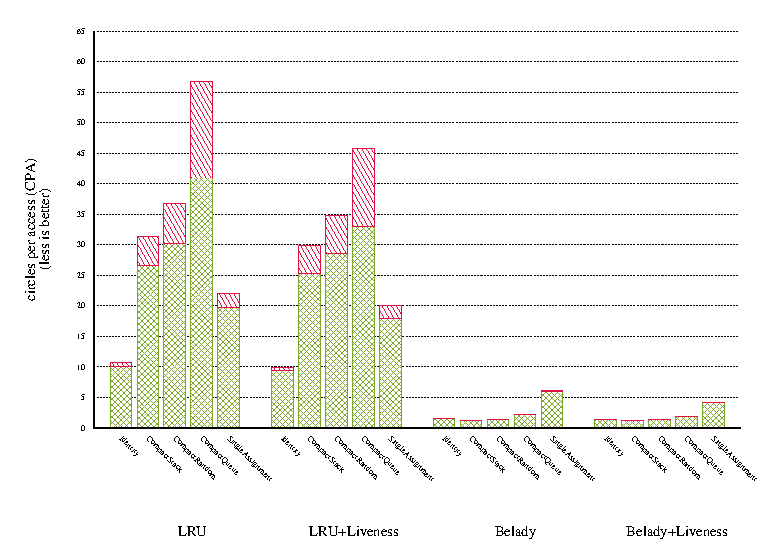
\includegraphics[width=\textwidth]{figs/plots/perf-misses-450-soplex.eps}
    \subcaption{Cache misses and cache hits}
  \end{subfigure}%
  \begin{subfigure}[b]{0.5\textwidth}%
    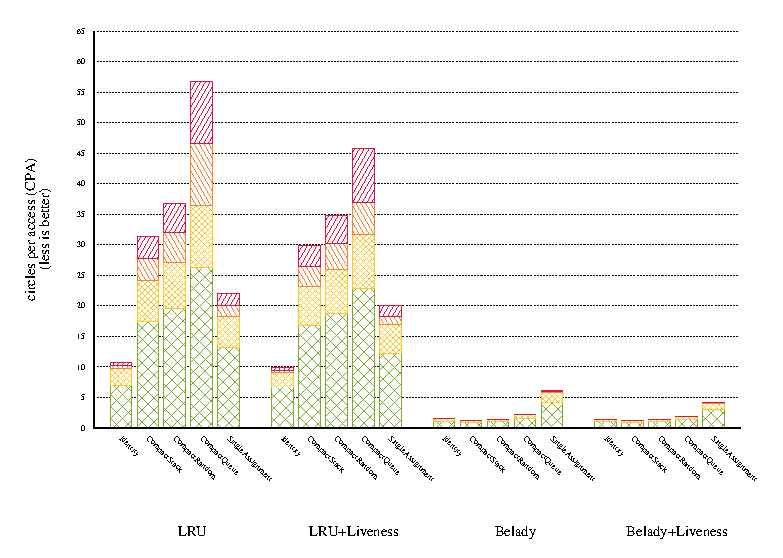
\includegraphics[width=\textwidth]{figs/plots/perf-450-soplex.eps}
    \subcaption{Types of memory operations}
  \end{subfigure}%
  \caption{Performance: 450.soplex}
  \label{fig:performance-450-soplex}
\end{figure}

\begin{figure}[!ht]
    \begin{subfigure}[b]{0.5\textwidth}%
    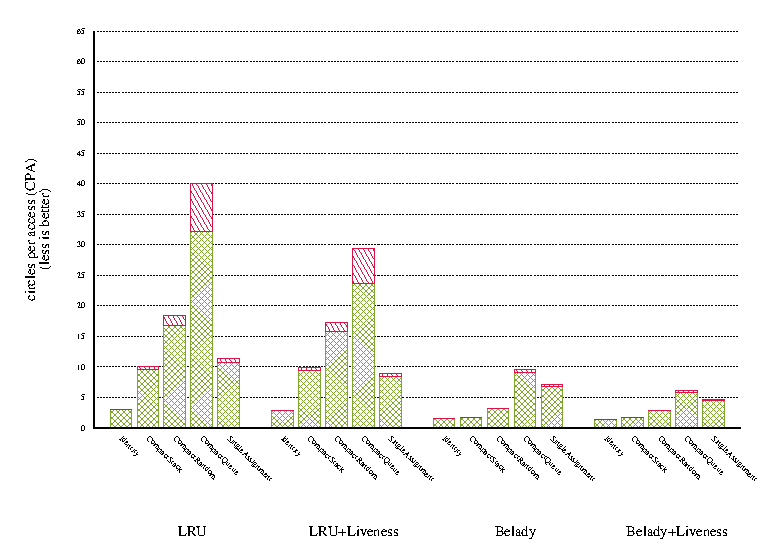
\includegraphics[width=\textwidth]{figs/plots/perf-misses-454-calculix.eps}
    \subcaption{Cache misses and cache hits}
  \end{subfigure}%
  \begin{subfigure}[b]{0.5\textwidth}%
    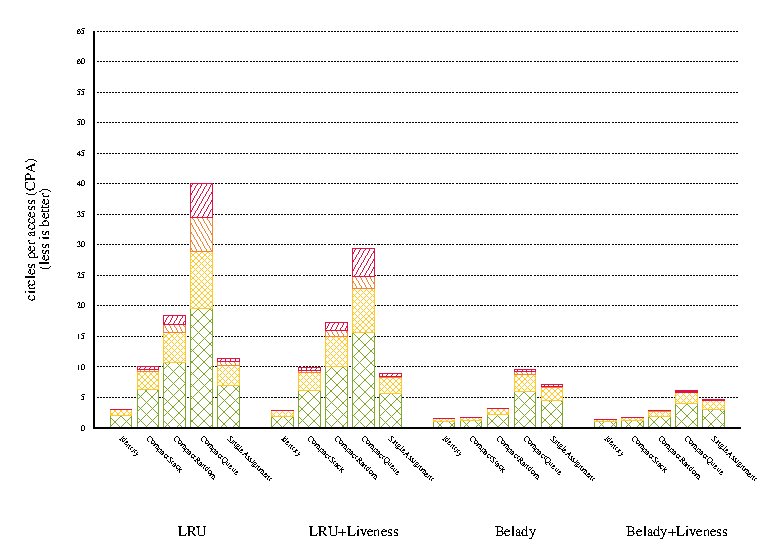
\includegraphics[width=\textwidth]{figs/plots/perf-454-calculix.eps}
    \subcaption{Types of memory operations}
  \end{subfigure}%
  \caption{Performance: 454.calculix}
  \label{fig:performance-454-calculix}
\end{figure}

\begin{figure}[!ht]
  \begin{subfigure}[b]{0.5\textwidth}%
    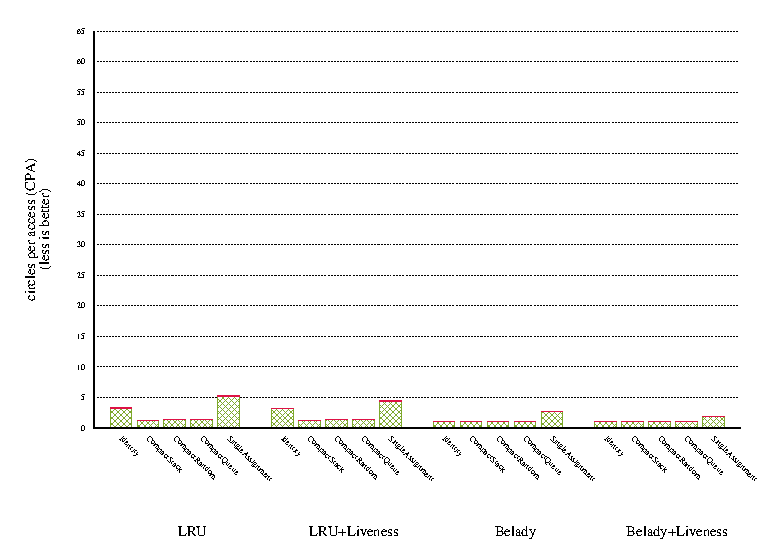
\includegraphics[width=\textwidth]{figs/plots/perf-misses-462-libquantum.eps}
    \subcaption{Cache misses and cache hits}
  \end{subfigure}%
  \begin{subfigure}[b]{0.5\textwidth}%
    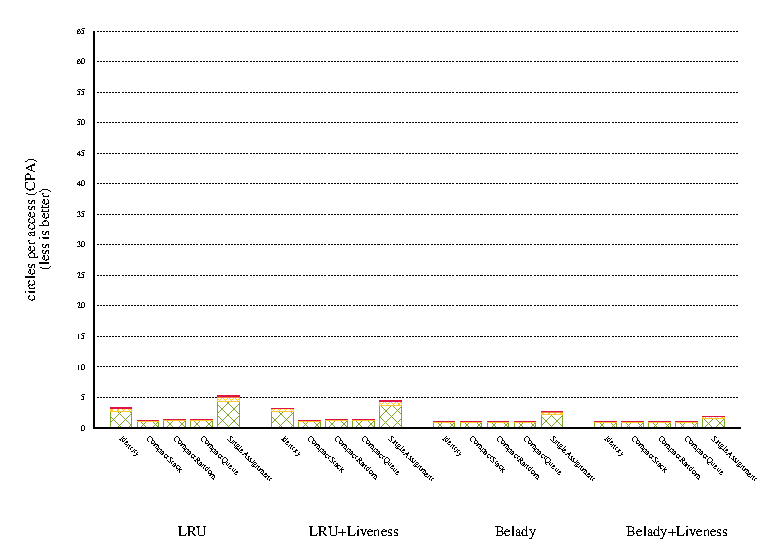
\includegraphics[width=\textwidth]{figs/plots/perf-462-libquantum.eps}
    \subcaption{Types of memory operations}
  \end{subfigure}%
  \caption{Performance: 462.libquantum}
  \label{fig:performance-462-libquantum}
\end{figure}

\begin{figure}[!ht]
  \begin{subfigure}[b]{0.5\textwidth}%
    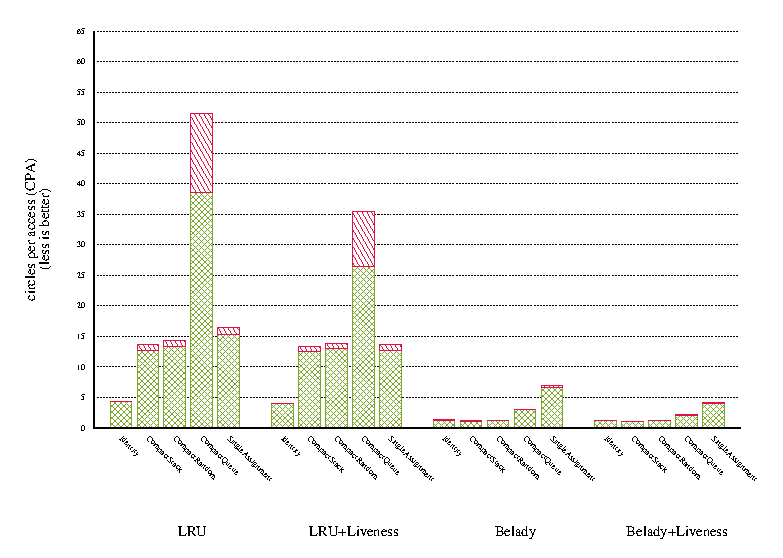
\includegraphics[width=\textwidth]{figs/plots/perf-misses-deltablue.eps}
    \subcaption{Cache misses and cache hits}
  \end{subfigure}%
  \begin{subfigure}[b]{0.5\textwidth}%
    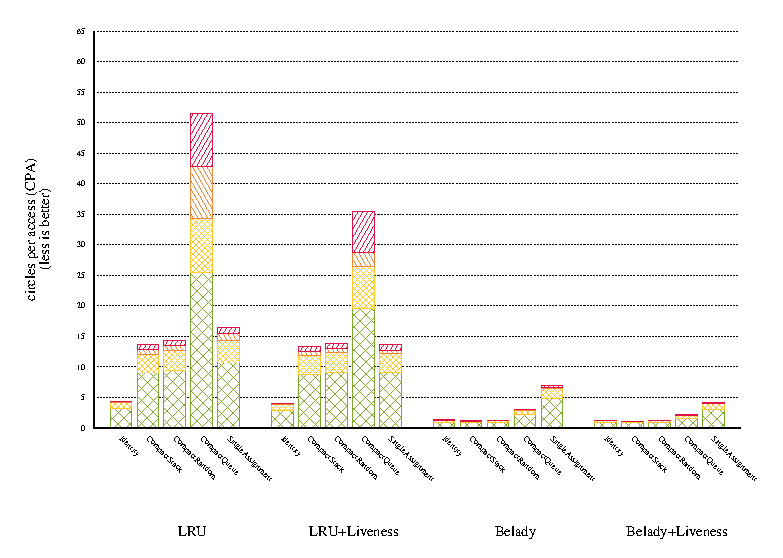
\includegraphics[width=\textwidth]{figs/plots/perf-deltablue.eps}
    \subcaption{Types of memory operations}
  \end{subfigure}%
  \caption{Performance: deltablue}
  \label{fig:performance-deltablue}
\end{figure}

\begin{figure}[!ht]
  \begin{subfigure}[b]{0.5\textwidth}%
    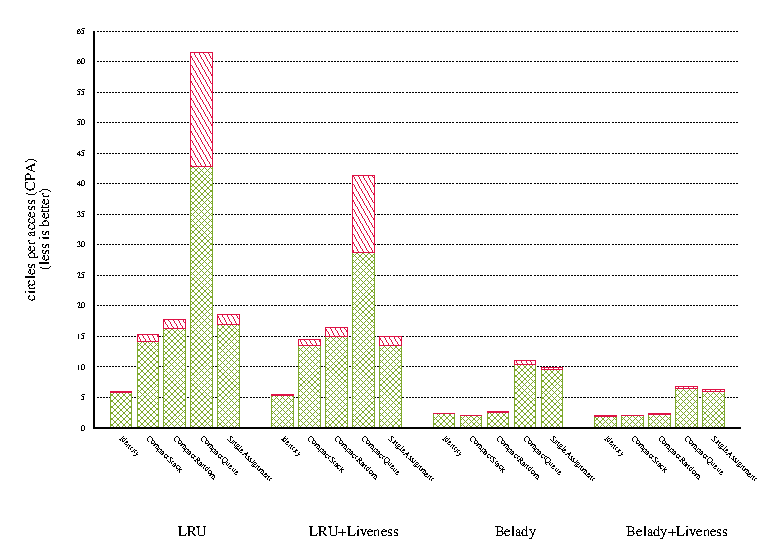
\includegraphics[width=\textwidth]{figs/plots/perf-misses-raytrace.eps}
    \subcaption{Cache misses and cache hits}
  \end{subfigure}%
  \begin{subfigure}[b]{0.5\textwidth}%
    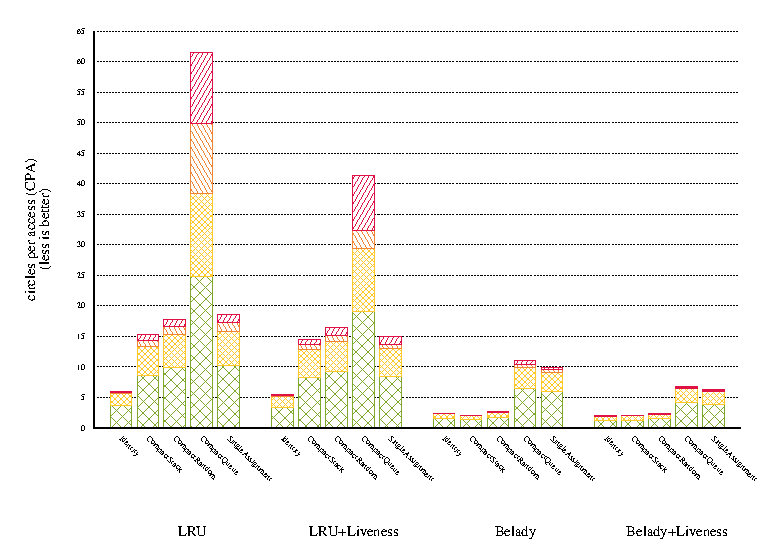
\includegraphics[width=\textwidth]{figs/plots/perf-raytrace.eps}
    \subcaption{Types of memory operations}
  \end{subfigure}%
  \caption{Performance: raytrace}
  \label{fig:performance-raytrace}
\end{figure}

\begin{figure}[!ht]
  \begin{subfigure}[b]{0.5\textwidth}%
    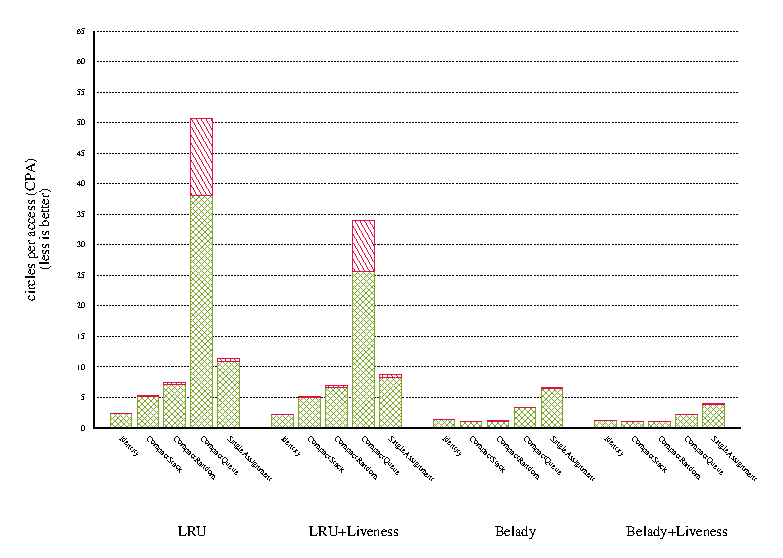
\includegraphics[width=\textwidth]{figs/plots/perf-misses-richards.eps}
    \subcaption{Cache misses and cache hits}
  \end{subfigure}%
  \begin{subfigure}[b]{0.5\textwidth}%
    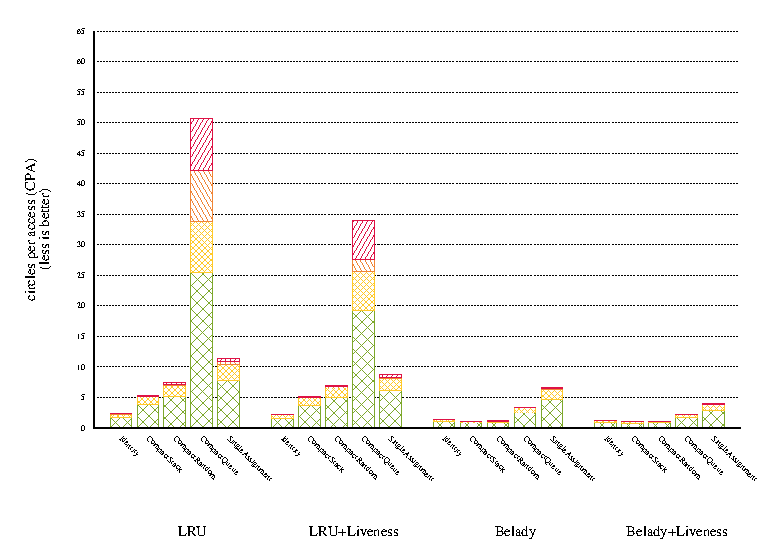
\includegraphics[width=\textwidth]{figs/plots/perf-richards.eps}
    \subcaption{Types of memory operations}
  \end{subfigure}%
  \caption{Performance: richards}
  \label{fig:performance-richards}
\end{figure}

\subsection{Speedup \& Compaction}\label{app:experiment-speedup-compaction}

\begin{figure}[!ht]
  \begin{subfigure}[b]{0.5\textwidth}%
    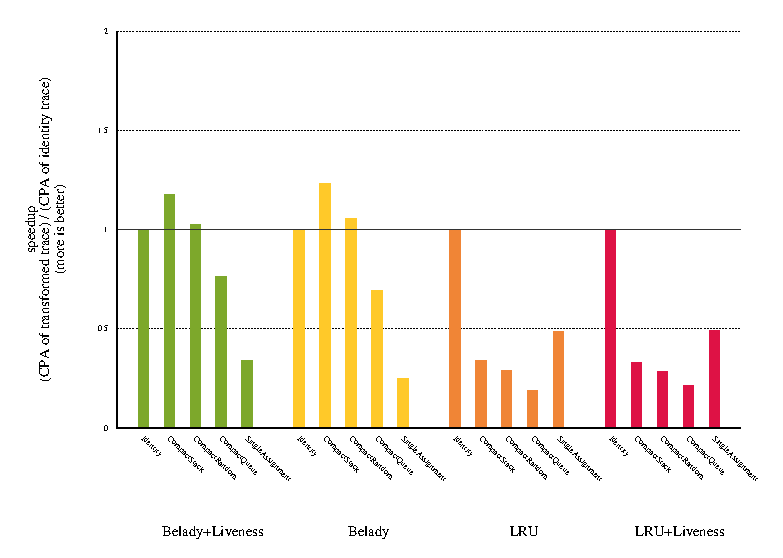
\includegraphics[width=\textwidth]{figs/plots/speedup-450-soplex.eps}
    \subcaption{Speedup}
  \end{subfigure}%
  \begin{subfigure}[b]{0.5\textwidth}%
    \includegraphics[width=\textwidth]{figs/plots/compaction-450-soplex.eps}
    \subcaption{Compaction}
  \end{subfigure}%
    \caption{Speedup \& Compaction: 450.soplex}
  \label{fig:speedup-compaction-450-soplex}
\end{figure}

\begin{figure}[!ht]
  \begin{subfigure}[b]{0.5\textwidth}%
    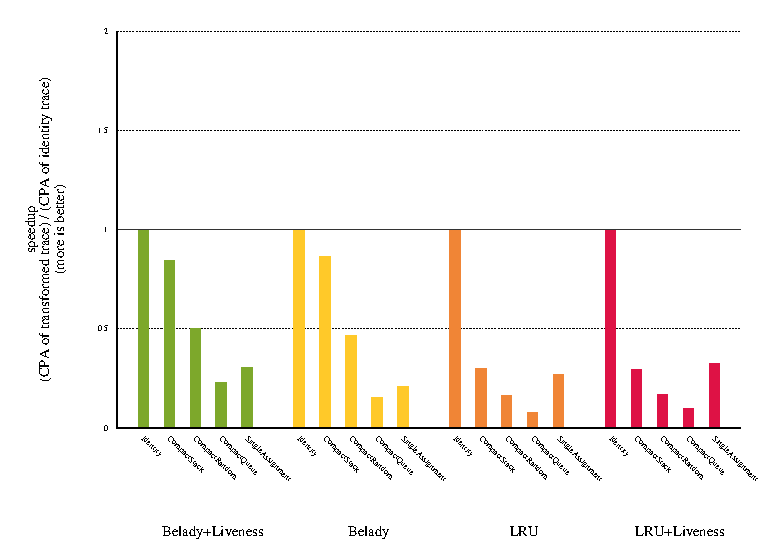
\includegraphics[width=\textwidth]{figs/plots/speedup-454-calculix.eps}
    \subcaption{Speedup}
  \end{subfigure}%
  \begin{subfigure}[b]{0.5\textwidth}%
    \includegraphics[width=\textwidth]{figs/plots/compaction-454-calculix.eps}
    \subcaption{Compaction}
  \end{subfigure}%
    \caption{Speedup \& Compaction: 454.calculix}
  \label{fig:speedup-compaction-454-calculix}
\end{figure}

\begin{figure}[!ht]
  \begin{subfigure}[b]{0.5\textwidth}%
    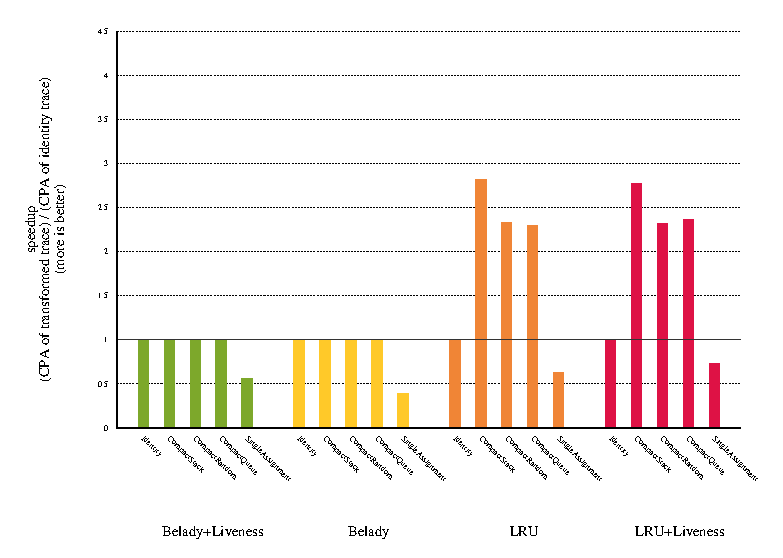
\includegraphics[width=\textwidth]{figs/plots/speedup-462-libquantum.eps}
    \subcaption{Speedup}
  \end{subfigure}%
  \begin{subfigure}[b]{0.5\textwidth}%
    \includegraphics[width=\textwidth]{figs/plots/compaction-462-libquantum.eps}
    \subcaption{Compaction}
  \end{subfigure}%
    \caption{Speedup \& Compaction: 462.libquantum}
  \label{fig:speedup-compaction-462-libquantum}
\end{figure}

\begin{figure}[!ht]
  \begin{subfigure}[b]{0.5\textwidth}%
    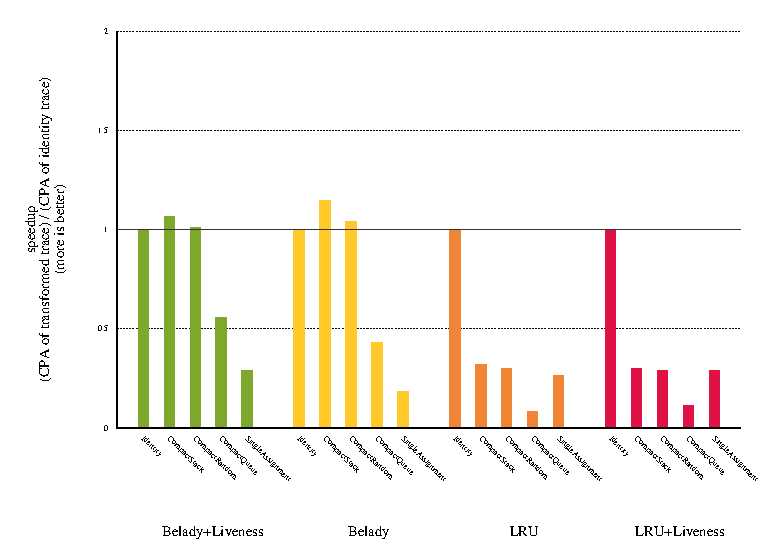
\includegraphics[width=\textwidth]{figs/plots/speedup-deltablue.eps}
    \subcaption{Speedup}
  \end{subfigure}%
  \begin{subfigure}[b]{0.5\textwidth}%
    \includegraphics[width=\textwidth]{figs/plots/compaction-deltablue.eps}
    \subcaption{Compaction}
  \end{subfigure}%
    \caption{Speedup \& Compaction: deltablue}
  \label{fig:speedup-compaction-deltablue}
\end{figure}

\begin{figure}[!ht]
  \begin{subfigure}[b]{0.5\textwidth}%
    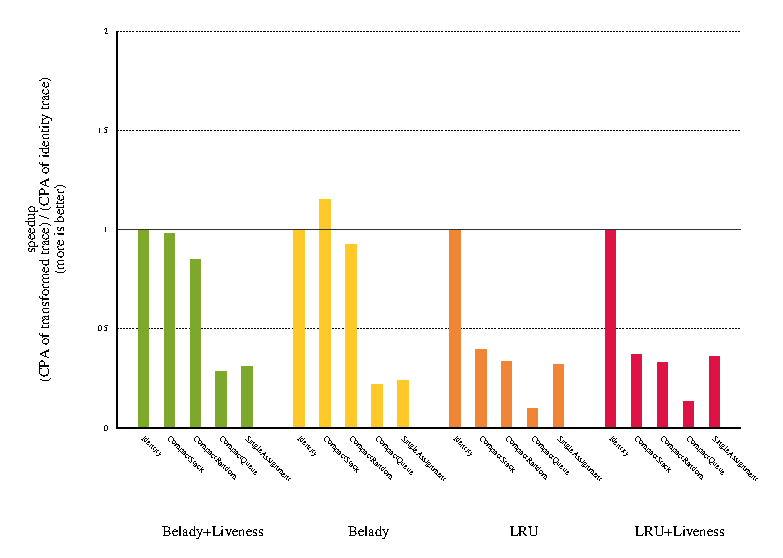
\includegraphics[width=\textwidth]{figs/plots/speedup-raytrace.eps}
    \subcaption{Speedup}
  \end{subfigure}%
  \begin{subfigure}[b]{0.5\textwidth}%
    \includegraphics[width=\textwidth]{figs/plots/compaction-raytrace.eps}
    \subcaption{Compaction}
  \end{subfigure}%
    \caption{Speedup \& Compaction: raytrace}
  \label{fig:speedup-compaction-raytrace}
\end{figure}

\begin{figure}[!ht]
  \begin{subfigure}[b]{0.5\textwidth}%
    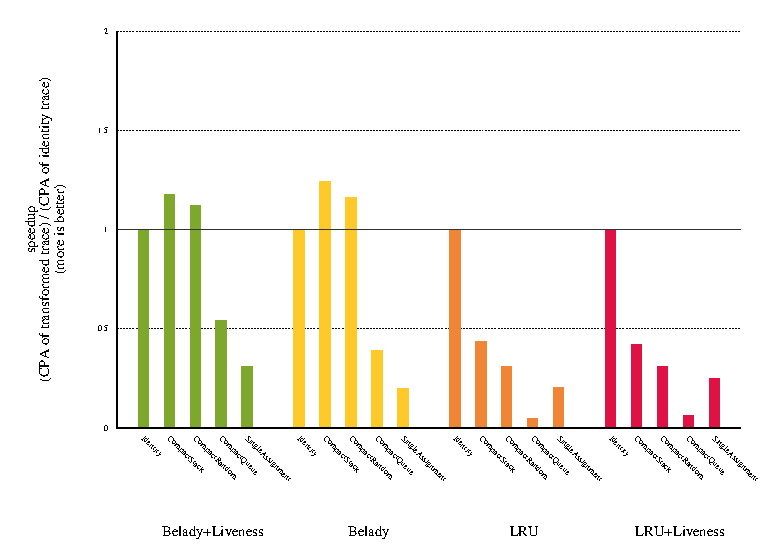
\includegraphics[width=\textwidth]{figs/plots/speedup-richards.eps}
    \subcaption{Speedup}
  \end{subfigure}%
  \begin{subfigure}[b]{0.5\textwidth}%
    \includegraphics[width=\textwidth]{figs/plots/compaction-richards.eps}
    \subcaption{Compaction}
  \end{subfigure}%
  \caption{Speedup \& Compaction: richards}
  \label{fig:speedup-compaction-richards}
\end{figure}

% \clearpage
\section{Digression on Caches}

This experimental section is distinguished into 2 parts. First we show a
few different opportunities to access a linked list, and an array,
respectively. Allows keeping our purpose in mind, we want to illustrate
the cache hierarchy. Secondly, we go into details and clarify a raising
question. Which finally leads to the answer we are looking for.

All experiments were executed on a MacBook Pro with a Intel(R) Core(TM)
i5-3230M CPU @ 2.60GHz and 3 cache levels (L1d=32KB, L1i=32KB, L2=256KB,
and L3=3MB). During the experiments there were other processes running
on the MacBook, this is why these results should be seen as proof of
concept.

\subsection{Configuration}\label{configuration-3}

The configuration is for all experiments identical.

\begin{longtable}[c]{@{}cccc@{}}
\toprule
Reps & Operations & Working Set Sizes & Addresses\tabularnewline
\midrule
\endhead
3 & 234 & 210 - 228 & 228\tabularnewline
\bottomrule
\end{longtable}

We are aware that the number of repetitions is very small, but we
consider these experiments as a \emph{proof of concept}. So 3
repetitions should be good enough.

There are parameters listed within the configuration files which are
\textbf{not} used for this experiments! These are only listed to keep
the experimental framework working.

\begin{itemize}
\tightlist
\item
  Fragmentation factor
\item
  Store ratio
\end{itemize}

As explained above we generate for each working set size a standalone
\texttt{C} file. which is complied with \texttt{gcc} in version 4.8.5
with following compiler flags \texttt{-std=c99} and \texttt{-O0}.

\hypertarget{access-opportunities}{\subsection{Access
opportunities}\label{access-opportunities}}

\hypertarget{linked-list}{\paragraph{Linked List}\label{linked-list}}

This section presents code snippets and performance results of accessing
a linked list to illustrate the cache hierarchy.

\hypertarget{sequential-access-with-2-loops}{\subparagraph{Sequential
access with 2 loops}\label{sequential-access-with-2-loops}}

The code snippet below shows how to access the linked list in a
sequential manner. All list elements are sequentially linked
corresponding to there position in (contiguous) memory. This approach
uses two nested loops.

\begin{Shaded}
\begin{Highlighting}[]
\DataTypeTok{static} \DataTypeTok{uint64_t} \NormalTok{access_read() \{}
  \KeywordTok{struct} \NormalTok{l * cur = &list[}\DecValTok{0}\NormalTok{];}
  \DataTypeTok{uint64_t} \NormalTok{start = getTimeMicrosecs();}
  \KeywordTok{for}\NormalTok{(}\DataTypeTok{int} \NormalTok{i = }\DecValTok{0}\NormalTok{; i < ITERS; i++)}
  \NormalTok{\{}
    \KeywordTok{for}\NormalTok{(}\DataTypeTok{int} \NormalTok{e = }\DecValTok{0}\NormalTok{; e < ELEMS; e++)}
    \NormalTok{\{}
      \NormalTok{cur = cur->n;}
      \NormalTok{(}\DataTypeTok{void}\NormalTok{)cur->pad[}\DecValTok{0}\NormalTok{];}
    \NormalTok{\}}
  \NormalTok{\}}
  \KeywordTok{return} \NormalTok{getTimeMicrosecs() - start;}
\NormalTok{\}}
\end{Highlighting}
\end{Shaded}

\Cref{ll-seqread-nl} presents the performance of the code above. As expected
the cache hierarchy is observable. However, performance is not that
good. How poor it really is illustrates the next experiment.

\begin{figure}[htbp]
\centering
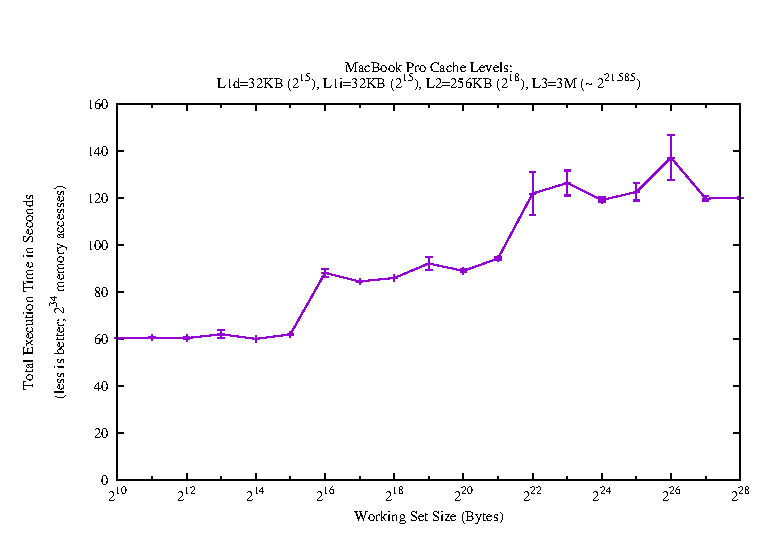
\includegraphics{appendix/plots-cache-measurements/plot-linked-list-2-loops}
\caption{Linked List, Sequential Read, and Nested Loop}
\label{ll-seqread-nl}
\end{figure}

\hypertarget{sequential-access-with-single-loop}{\subparagraph{Sequential
access with single loop}\label{sequential-access-with-single-loop}}

This approach is similar to the one above, but instead of two nested
loops a single loop is used. All list elements are sequentially linked
corresponding to there position in (contiguous) memory.

\begin{Shaded}
\begin{Highlighting}[]
\DataTypeTok{static} \DataTypeTok{uint64_t} \NormalTok{access_read() \{}
  \KeywordTok{struct} \NormalTok{l * cur = &list[}\DecValTok{0}\NormalTok{];}
  \DataTypeTok{uint64_t} \NormalTok{start = getTimeMicrosecs();}
  \KeywordTok{for}\NormalTok{(}\DataTypeTok{int} \NormalTok{i = }\DecValTok{0}\NormalTok{; i < ITERS * ELEMS; i++)}
  \NormalTok{\{}
    \NormalTok{cur = cur->n;}
    \NormalTok{(}\DataTypeTok{void}\NormalTok{)cur->pad[}\DecValTok{0}\NormalTok{];}
  \NormalTok{\}}
  \KeywordTok{return} \NormalTok{getTimeMicrosecs() - start;}
\NormalTok{\}}
\end{Highlighting}
\end{Shaded}

\Cref{app:ll-seqread-sl} illustrates the performance of the code from above. As
expected the results shows the typical shape. Remember the experiment
was not the only job running, this is why the shape not totally sharp.
This figure is used as baseline for the following experiments.

\begin{figure}[htbp]
\centering
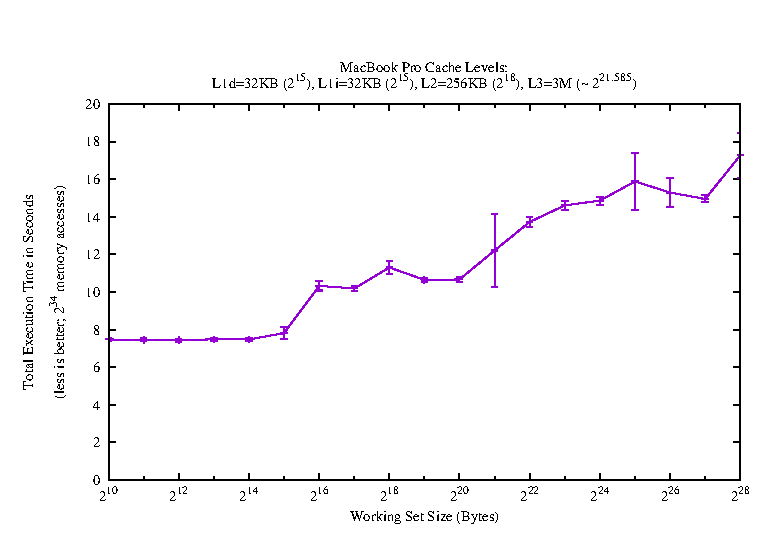
\includegraphics{appendix/plots-cache-measurements/plot-linked-list}
\caption{Linked List, Sequential Read, and Single Loop}
\label{app:ll-seqread-sl}
\end{figure}

\hypertarget{array}{\paragraph{Array}\label{array}}

This section presents different ways to compute the index of the array.
The aim is illustrate the influence of computing the index of the
current element on the actual measurements.

\hypertarget{sequential-access-with-2-loops-1}{\subparagraph{Sequential
access with 2 loops}\label{sequential-access-with-2-loops-1}}

The code snippet below shows how the array is accessed. This approach
uses to nested loop. The outer-one determines the number accesses on a
single element with the array. The inner-one ensures that keep walking
through the array.

\begin{Shaded}
\begin{Highlighting}[]
\DataTypeTok{static} \DataTypeTok{uint64_t} \NormalTok{access_read() \{}
  \DataTypeTok{uint64_t} \NormalTok{start = getTimeMicrosecs();}
  \KeywordTok{for}\NormalTok{(}\DataTypeTok{int} \NormalTok{i = }\DecValTok{0}\NormalTok{; i < ITERS; i++)}
    \KeywordTok{for}\NormalTok{(}\DataTypeTok{int} \NormalTok{j = }\DecValTok{0}\NormalTok{; j < ELEMS; j++)}
      \NormalTok{(}\DataTypeTok{void}\NormalTok{)list[j].pad[}\DecValTok{0}\NormalTok{];}
  \KeywordTok{return} \NormalTok{getTimeMicrosecs() - start;}
\NormalTok{\}}
\end{Highlighting}
\end{Shaded}

\Cref{app:arr-seqread-nl} presents the performance of the code above. Obviously
the cache hierarchy is not observable. Instead the performance seams to
be independent of the working set size. We continue with a few more
experiments on array before taking a closer look at this effect.

\begin{figure}[htbp]
\centering
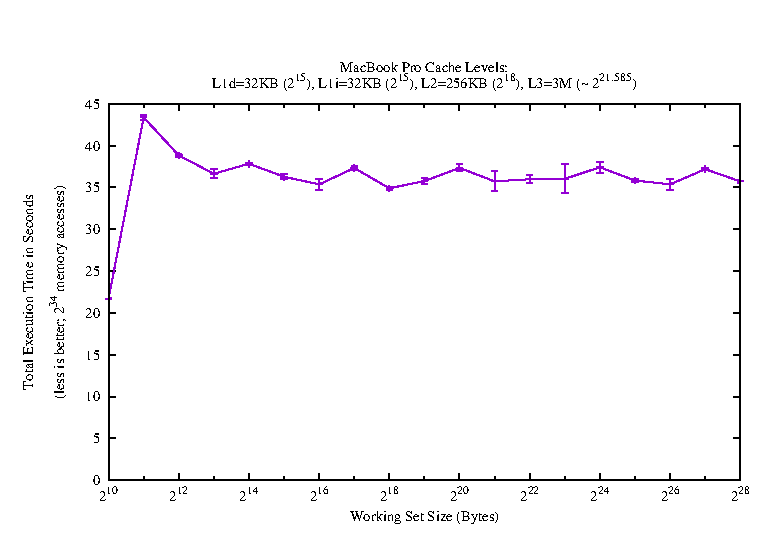
\includegraphics{appendix/plots-cache-measurements/plot-array-2-loops}
\caption{Array, Sequential Read, and Nested Loop}
\label{app:arr-seqread-nl}
\end{figure}

\hypertarget{sequential-access-with-single-loop-and-modulo}{\subparagraph{Sequential
access with single loop and
modulo}\label{sequential-access-with-single-loop-and-modulo}}

The code snippet below illustrates an approach which uses only one loop.
This requires a modulo operation to ensure to stay within the array
bounds.

\begin{Shaded}
\begin{Highlighting}[]
\DataTypeTok{static} \DataTypeTok{uint64_t} \NormalTok{access_read() \{}
  \DataTypeTok{uint64_t} \NormalTok{start = getTimeMicrosecs();}
  \KeywordTok{for}\NormalTok{(}\DataTypeTok{int} \NormalTok{i = }\DecValTok{0}\NormalTok{; i < ITERS * ELEMS; i++)}
    \NormalTok{(}\DataTypeTok{void}\NormalTok{)list[i%ELEMS].pad[}\DecValTok{0}\NormalTok{];}
  \KeywordTok{return} \NormalTok{getTimeMicrosecs() - start;}
\NormalTok{\}}
\end{Highlighting}
\end{Shaded}

\Cref{app:arr-seqread-sl} shows the performance of the code above. Again the
performance seams to be independent of the working set size. However,
there is a significant performance improvement compared to the approach
with two loops.

\begin{figure}[htbp]
\centering
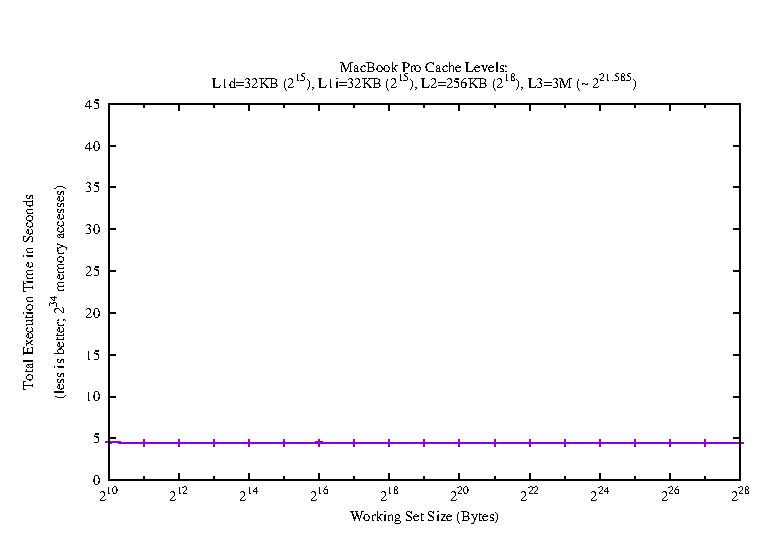
\includegraphics{appendix/plots-cache-measurements/plot-array-modulo-seq}
\caption{Array, Sequential Read, and Single Loop}
\label{app:arr-seqread-sl}
\end{figure}

\hypertarget{sequential-access-with-single-loop-and-modulo-linked-list-style}{\subparagraph{Sequential
access with single loop and modulo (linked list
style)}\label{sequential-access-with-single-loop-and-modulo-linked-list-style}}

The code snipped below presents an approach which used only one loop,
which requires a modulo operation to care about the array bounds.
Further, the coding style is like used a linked lists. There is an
additional variable \texttt{cur} which holds the address of the element
to access. The reason for this experiment that all experiments with
arrays so far do not show the cache hierarchy. To become as comparable
as possible we use this linked list like syntax.

\begin{Shaded}
\begin{Highlighting}[]
\DataTypeTok{static} \DataTypeTok{uint64_t} \NormalTok{access_read() \{}
  \KeywordTok{struct} \NormalTok{l * cur = &list[}\DecValTok{0}\NormalTok{];}
  \DataTypeTok{uint64_t} \NormalTok{start = getTimeMicrosecs();}
  \KeywordTok{for}\NormalTok{(}\DataTypeTok{int} \NormalTok{i = }\DecValTok{0}\NormalTok{; i < ITERS * ELEMS; i++)\{}
    \NormalTok{cur = &list[i%ELEMS];}
    \NormalTok{(}\DataTypeTok{void}\NormalTok{)cur->pad[}\DecValTok{0}\NormalTok{];}
  \NormalTok{\}}
  \KeywordTok{return} \NormalTok{getTimeMicrosecs() - start;}
\NormalTok{\}}
\end{Highlighting}
\end{Shaded}

\Cref{app:array-seqread-sl} below shows the performance of the code above. Again the
performance seams to be independent of the working set size. However,
the performance is slightly worse than the performance of the previous
experiment. The explanation is as simple as: It is requires to store the
address within \texttt{cur}, the approach from above computes address
and stores it in a register.

\begin{figure}[htbp]
\centering
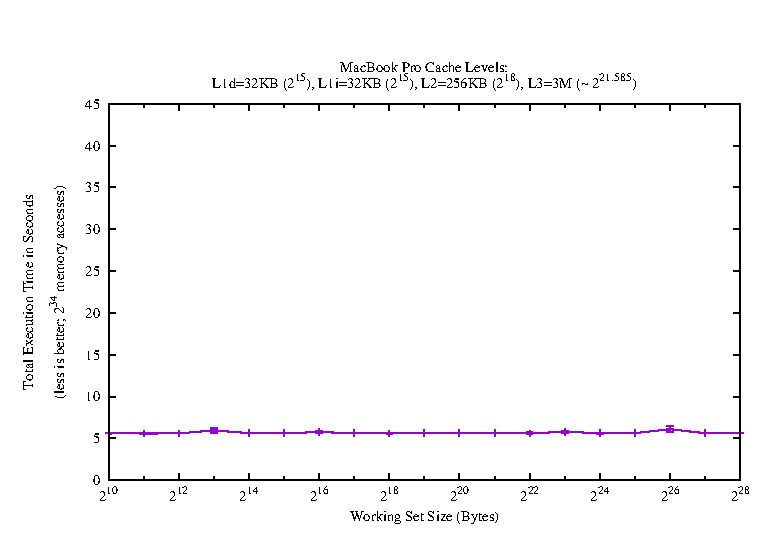
\includegraphics{appendix/plots-cache-measurements/plot-array-modulo-seq-2}
\caption{Array, Sequential Read, and Single Loop}
\label{app:array-seqread-sl}
\end{figure}

\hypertarget{sequential-access-with-single-loop-and-modulo-read-whole-payload}{\subparagraph{Sequential
access with single loop and modulo (read whole
payload)}\label{sequential-access-with-single-loop-and-modulo-read-whole-payload}}

The code snippet below presents an approach similar to those from above
with one difference: The whole payload is read (instead of simply
reading on element).

\begin{Shaded}
\begin{Highlighting}[]
\DataTypeTok{static} \DataTypeTok{uint64_t} \NormalTok{access_read() \{}
  \KeywordTok{struct} \NormalTok{l * cur = &list[}\DecValTok{0}\NormalTok{];}
  \DataTypeTok{uint64_t} \NormalTok{start = getTimeMicrosecs();}
  \KeywordTok{for}\NormalTok{(}\DataTypeTok{int} \NormalTok{i = }\DecValTok{0}\NormalTok{; i < ITERS * ELEMS; i++)\{}
    \NormalTok{cur = &list[i%ELEMS];}
    \KeywordTok{for}\NormalTok{(}\DataTypeTok{int} \NormalTok{j = }\DecValTok{0}\NormalTok{; j < NPAD; j++)}
      \NormalTok{(}\DataTypeTok{void}\NormalTok{)cur->pad[j];}
  \NormalTok{\}}
  \KeywordTok{return} \NormalTok{getTimeMicrosecs() - start;}
\NormalTok{\}}
\end{Highlighting}
\end{Shaded}

\Cref{app:array-seqreadall-sl} shows the result of the code from above. It was
expected to see the cache hierarchy, because we read the whole array
which is definitely larger than the cache. Nevertheless, the result is
the same as for the other array experiments. The only difference is the
worse performance yield by the additional loop.

\begin{figure}[htbp]
\centering
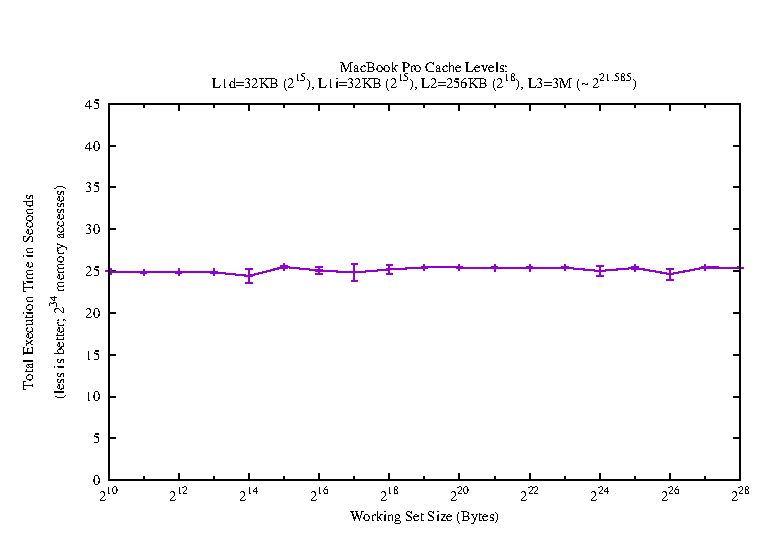
\includegraphics{appendix/plots-cache-measurements/plot-array-modulo-seq-read-all}
\caption{Array, Sequential Read All, and Single Loop}
\label{app:array-seqreadall-sl}
\end{figure}

\hypertarget{random-access-with-single-loop-and-modulo}{\subparagraph{Random
access with single loop and
modulo}\label{random-access-with-single-loop-and-modulo}}

The code snippet below presents an approach similar to those from above
with one difference: Now the array elements are access in a random
order. \texttt{mapper} contains a randomly chosen permutation of all
array indexes.

\begin{Shaded}
\begin{Highlighting}[]
\DataTypeTok{static} \DataTypeTok{uint64_t} \NormalTok{access_read() \{}
  \KeywordTok{struct} \NormalTok{l * cur = &list[}\DecValTok{0}\NormalTok{];}
  \DataTypeTok{uint64_t} \NormalTok{start = getTimeMicrosecs();}
  \KeywordTok{for}\NormalTok{(}\DataTypeTok{int} \NormalTok{i = }\DecValTok{0}\NormalTok{; i < ITERS * ELEMS; i++)\{}
    \NormalTok{cur = &list[mapper[i%ELEMS]];}
    \NormalTok{(}\DataTypeTok{void}\NormalTok{)cur->pad[}\DecValTok{0}\NormalTok{];}
  \NormalTok{\}}
  \KeywordTok{return} \NormalTok{getTimeMicrosecs() - start;}
\NormalTok{\}}
\end{Highlighting}
\end{Shaded}

The performance result is shown in \Cref{app:arr-randread-sl}. The random access order is chosen
to get rid of pre-fetching which could probably influence the execution
time. But even with random access on the array we cannot observer the
cache hierarchy. It is comparable to \emph{sequential access with single
loop and modulo (linked list style)}.

\begin{figure}[htbp]
\centering
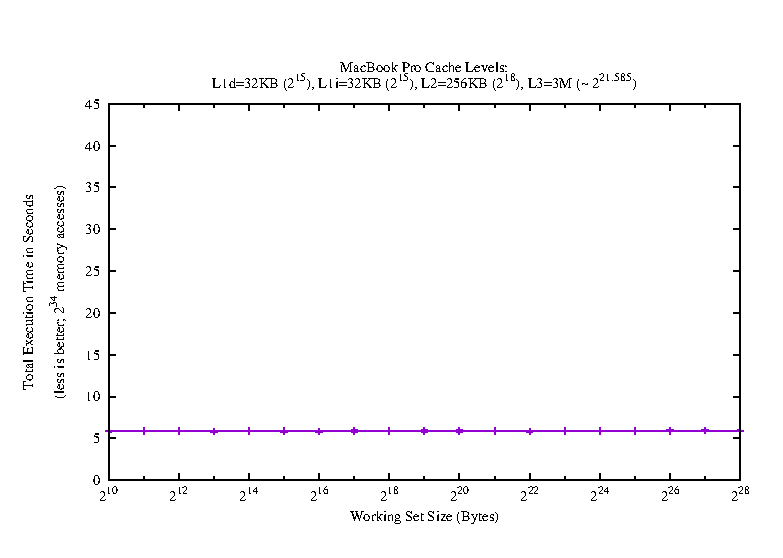
\includegraphics{appendix/plots-cache-measurements/plot-array-modulo-rand}
\caption{Array, Random Read, and Single Loop}
\label{app:arr-randread-sl}
\end{figure}

\hypertarget{summary-1}{\paragraph{Summary}\label{summary-1}}

We presented experiments on accessing two different data structures,
linked lists, and arrays, respectively. For linked lists we showed that
there is a huge performance difference in using nested loops or just a
single loop. This fact is not super surprising, but nevertheless
important to keep in mind. Also for arrays is shown that 2 nested loops
perform do not perform well. Further, we tried to measure the cache
hierarchy using just an array. Without success. Instead our experiments
show the performance differences of the different ways to access an
array. The following section will go into details why performance seams
to be independent of the working set size.

\hypertarget{the-problem}{\subsection{The problem}\label{the-problem}}

\hypertarget{definition}{\subsection{Definition}\label{definition}}

The performance curve of all experiments with array only is close to a
horizontal line, and this is unexpected behavior. It seams to be
independent of the working set size. The expected behavior would be
similar to the linked list experiments, which illustrate the cache
hierarchy.

\subsection{Analysis}\label{analysis-1}

In this section we investigate the unexpected behavior of our array
experiments from above. These experiments present constant performance
independent of the working set size.

\hypertarget{assembly-code-analysis}{\paragraph{Assembly code
analysis}\label{assembly-code-analysis}}

To simplify as much as possible we inspect only 2 code snippets from
above: - Linked list with single loop and - Array with single loop in
linked list style.

These two are the most similar one so optimal for comparison. We
disassembled the executables complied on the MacBook mentioned above.
For disassembling we are using an on-line disassembler:
\url{https://onlinedisassembler.com}.

\textbf{Linked list: C code}

\begin{Shaded}
\begin{Highlighting}[]
\DataTypeTok{static} \DataTypeTok{uint64_t} \NormalTok{access_read() \{}
  \KeywordTok{struct} \NormalTok{l * cur = &list[}\DecValTok{0}\NormalTok{];}
  \DataTypeTok{uint64_t} \NormalTok{start = getTimeMicrosecs();}
  \KeywordTok{for}\NormalTok{(}\DataTypeTok{int} \NormalTok{i = }\DecValTok{0}\NormalTok{; i < ITERS * ELEMS; i++)\{}
    \NormalTok{cur = cur->n;}
    \NormalTok{(}\DataTypeTok{void}\NormalTok{)cur->pad[}\DecValTok{0}\NormalTok{];}
  \NormalTok{\}}
  \KeywordTok{return} \NormalTok{getTimeMicrosecs() - start;}
\NormalTok{\}}
\end{Highlighting}
\end{Shaded}

\textbf{Linked list: Assembly}

\begin{verbatim}
100000ec0 <_access_read>:
100000ec0 55                     push   %rbp
100000ec1 4889e5                 mov    %rsp,         %rbp
100000ec4 4883ec20               sub    $0x20,        %rsp
100000ec8 488d0551010000         lea    0x151(%rip),  %rax # 0x100001020<_list>
100000ecf 488945f8               mov    %rax,         -0x8(%rbp)
100000ed3 e858000000             callq  0x100000f30   <_getTimeMicrosecs>
100000ed8 488945f0               mov    %rax,         -0x10(%rbp)
100000edc c745ec00000000         movl   $0x0,         -0x14(%rbp)
100000ee3 48b80000000004000000   movabs $0x400000000, %rax
100000eed 48634dec               movslq -0x14(%rbp),  %rcx
100000ef1 4839c1                 cmp    %rax,         %rcx
100000ef4 0f8319000000           jae    0x100000f13
100000efa 488b45f8               mov    -0x8(%rbp),   %rax
100000efe 488b00                 mov    (%rax),       %rax
100000f01 488945f8               mov    %rax,         -0x8(%rbp)
100000f05 8b45ec                 mov    -0x14(%rbp),  %eax
100000f08 83c001                 add    $0x1,         %eax
100000f0b 8945ec                 mov    %eax,         -0x14(%rbp)
100000f0e e9d0ffffff             jmpq   0x100000ee3
100000f13 e818000000             callq  0x100000f30   <_getTimeMicrosecs>
100000f18 482b45f0               sub    -0x10(%rbp),  %rax
100000f1c 4883c420               add    $0x20,        %rsp
100000f20 5d                     pop    %rbp
100000f21 c3                     retq   
\end{verbatim}

\textbf{Array: C code}

\begin{Shaded}
\begin{Highlighting}[]
\NormalTok{...}
\DataTypeTok{static} \DataTypeTok{uint64_t} \NormalTok{access_read() \{}
  \KeywordTok{struct} \NormalTok{l * cur = &list[}\DecValTok{0}\NormalTok{];}
  \DataTypeTok{uint64_t} \NormalTok{start = getTimeMicrosecs();}
  \KeywordTok{for}\NormalTok{(}\DataTypeTok{int} \NormalTok{i = }\DecValTok{0}\NormalTok{; i < ITERS * ELEMS; i++)\{}
    \NormalTok{cur = &list[i%ELEMS];}
    \NormalTok{(}\DataTypeTok{void}\NormalTok{)cur->pad[}\DecValTok{0}\NormalTok{];}
  \NormalTok{\}}
  \KeywordTok{return} \NormalTok{getTimeMicrosecs() - start;}
\NormalTok{\}}
\end{Highlighting}
\end{Shaded}

\textbf{Array: Assembly}

\begin{verbatim}
100000eb0 <_access_read>:
100000eb0 55                     push   %rbp
100000eb1 4889e5                 mov    %rsp,         %rbp
100000eb4 4883ec20               sub    $0x20,        %rsp
100000eb8 488d0561010000         lea    0x161(%rip),  %rax # 0x100001020<_list>
100000ebf 488945f8               mov    %rax,         -0x8(%rbp)
100000ec3 e868000000             callq  0x100000f30   <_getTimeMicrosecs>
100000ec8 488945f0               mov    %rax,         -0x10(%rbp)
100000ecc c745ec00000000         movl   $0x0,         -0x14(%rbp)
100000ed3 48b80000000004000000   movabs $0x400000000, %rax
100000edd 48634dec               movslq -0x14(%rbp),  %rcx
100000ee1 4839c1                 cmp    %rax,         %rcx
100000ee4 0f8328000000           jae    0x100000f12
100000eea 488d052f010000         lea    0x12f(%rip),  %rax # 0x100001020<_list>
100000ef1 48634dec               movslq -0x14(%rbp),  %rcx
100000ef5 4883e10f               and    $0xf,         %rcx
100000ef9 48c1e106               shl    $0x6,         %rcx
100000efd 4801c8                 add    %rcx,         %rax
100000f00 488945f8               mov    %rax,         -0x8(%rbp)
100000f04 8b45ec                 mov    -0x14(%rbp),  %eax
100000f07 83c001                 add    $0x1,         %eax
100000f0a 8945ec                 mov    %eax,         -0x14(%rbp)
100000f0d e9c1ffffff             jmpq   0x100000ed3
100000f12 e819000000             callq  0x100000f30   <_getTimeMicrosecs>
100000f17 482b45f0               sub    -0x10(%rbp),  %rax
100000f1b 4883c420               add    $0x20,        %rsp
100000f1f 5d                     pop    %rbp
100000f20 c3                     retq   
\end{verbatim}

Now we remove everything this two code snippets have in common and is
not required for our analysis. What remains should help us to understand
the difference between array and linked list. Hopefully it offers some
answers about the performance differences.

Obviously, there are only a few lines which distinguishes the code
snippets. We take only a look at the code within the loop.

The code for the linked list is quite strait. First the address of
\texttt{cur} is loaded into \texttt{rax}. Next the address of \texttt{n}
is computed. Since \texttt{n} is the first element within the
\texttt{struct} this is identical with the address of \texttt{cur}.
Finally, the address stored in \texttt{n} is moved/assigned to
\texttt{cur} itself. For reading the first element of the payload there
is no command.

The code for the array consists of a few more lines. The most important
command is the \texttt{lea} command. \texttt{lea} is a special command
available on Intel x86 architectures. This is a so called \textbf{load
effective address} instruction, designed specially of arrays. It
performs a calculation of the effective operand address, but instead of
acting on that memory location, it loads the address that would have
been accessed into a register. This and the fact that there is no
assembly instruction generated for
\texttt{(void)\ cur-\textgreater{}pad{[}0{]}} are the reasons why the
performance of arrays seams to be independent of working set size. There
is no actual memory access, the way we want it. The following
instructions do the modulo computation and finally assign the computed
address to \texttt{cur} again.

\begin{verbatim}
# linked list
<_access_read>:
loop:     ...
          jae    end_loop
          mov    -0x8(%rbp),   %rax       # load address of cur
          mov    (%rax),       %rax       # compute address of n
          mov    %rax,         -0x8(%rbp) # assignment: cur = cur->n
                                          # (void) cur->pad[0]
          ...                             # increment loop counter
          jmpq   loop
end_loop: ...

# array
<_access_read>:
loop:     ...
          jae    end_loop
          lea    0x12f(%rip),  %rax       # load list address
          movslq -0x14(%rbp),  %rcx       # load max. loop counter
          and    $0xf,         %rcx       # compute: i%ELEMS
          shl    $0x6,         %rcx       # compute: i%ELEMS
          add    %rcx,         %rax       # compute address of list element
          mov    %rax,         -0x8(%rbp) # assignment: cur = &list[i%ELEMS]
                                          # (void) cur->pad[0]
          ...                             # increment loop counter
          jmpq   loop
end_loop: ...
\end{verbatim}

\textbf{Explanations:} - Source:
\href{https://en.wikipedia.org/wiki/X86_instruction_listings}{Wikipedia}
- Variables + \texttt{-0x8(\%rbp)}: current element
(\texttt{struct\ l\ *cur}) + \texttt{-0x14(\%rbp)}: loop counter
(\texttt{int\ i}) + \texttt{0x12f(\%rip)}: the list of structs
(\texttt{struct\ list{[}ELEMS{]}}) + \texttt{\$0xf}: number of elements
(\texttt{ELEMS} = 16) + \texttt{\$0x6}: decimal number \texttt{6} -
Registers + \texttt{rax}, \texttt{rbx}, \texttt{rcx}: 64-bit register +
\texttt{rbp}: 64-bit register, holds method local variables +
\texttt{rip}: 64-bit instruction pointer register. only in the 64-bit
mode it is possible to reference data relative to the instruction
pointer, less copying of data is required. - Commands +
\texttt{movslq\ S,\ R}: Move sign-extended double word + \texttt{shl}:
Shift left + \texttt{lea}: ``Some instruction set architectures, such as
Intel x86 {[}\ldots{}{]}, have a \textbf{Load effective address}
instruction.{[}\ldots{}{]} This performs a calculation of the effective
operand address, but instead of acting on that memory location, it loads
the address that would have been accessed into a register.
{[}\ldots{}{]}'' \emph{Source:
\href{https://en.wikipedia.org/wiki/Addressing_mode\#Useful_side_effect}{Wikipedia}}

\hypertarget{further-investigations}{\paragraph{Further
investigations}\label{further-investigations}}

One issue which is identified above is that probably there are no
Assembly commands generated for the \texttt{C} code line
\texttt{(void)\ cur-\textgreater{}pad{[}0{]};}. This is not only an
issue of our array experiments. Also for the linked list experiments
these Assembly commands are missing. For simplicity reason the following
investigations are based on the linked list code. Since there are less
Assembly commands generated in total.

\hypertarget{without-accessing-pad}{\subparagraph{\texorpdfstring{Without
accessing
\texttt{pad}}{Without accessing pad}}\label{without-accessing-pad}}

This first experiment is used to confirm or refute the hypotheses that
the compiler does not generate Assembly commands for the access of
\texttt{pad}. For this purpose we remove the line
\texttt{(void)\ cur-\textgreater{}pad{[}0{]};} for the \texttt{C} code
re-compile it and again inspect it with disassembler used before
(\url{https://onlinedisassembler.com}). Both code snippets are presented
below.

\begin{Shaded}
\begin{Highlighting}[]
\DataTypeTok{static} \DataTypeTok{uint64_t} \NormalTok{access_read() \{}
  \KeywordTok{struct} \NormalTok{l * cur = &list[}\DecValTok{0}\NormalTok{];}
  \DataTypeTok{uint64_t} \NormalTok{start = getTimeMicrosecs();}
  \KeywordTok{for}\NormalTok{(}\DataTypeTok{int} \NormalTok{i = }\DecValTok{0}\NormalTok{; i < ITERS * ELEMS; i++)\{}
    \NormalTok{cur = cur->n;}
  \NormalTok{\}}
  \KeywordTok{return} \NormalTok{getTimeMicrosecs() - start;}
\NormalTok{\}}
\end{Highlighting}
\end{Shaded}

\begin{verbatim}
<_access_read>:
loop:     ...
          jae end_loop
          mov -0x8(%rbp),     %rax        # load address of cur
          mov (%rax),         %rax        # compute address of n
          mov %rax,           -0x8(%rbp)  # assignment: cur = cur->n
          ...                             # increment loop counter
          jmpq loop
end_loop: ...
\end{verbatim}

(\href{https://github.com/cksystemsgroup/SemanticLocality/blob/localizer/experiments/localizer/__meeting_20161130/assembly_tests/exp_ll_remove_cmd.txt}{complete
assembly code})

Obviously, the disassembled code is identically with the code generated
with one line more. This is why the Assembly code from above confirms
our hypotheses: There is no code generated for the \texttt{C} code
\texttt{(void)\ cur-\textgreater{}pad{[}0{]};}. Next we want to know it
the cast is the reason or line itself.

\hypertarget{remove-cast}{\subparagraph{Remove cast}\label{remove-cast}}

To find out why the compiler ignores
\texttt{(void)\ cur-\textgreater{}pad{[}0{]};} we remove the cast. This
raises a compiler warning of an unused variable.

\begin{Shaded}
\begin{Highlighting}[]
\DataTypeTok{static} \DataTypeTok{uint64_t} \NormalTok{access_read() \{}
  \KeywordTok{struct} \NormalTok{l * cur = &list[}\DecValTok{0}\NormalTok{];}
  \DataTypeTok{uint64_t} \NormalTok{start = getTimeMicrosecs();}
  \KeywordTok{for}\NormalTok{(}\DataTypeTok{int} \NormalTok{i = }\DecValTok{0}\NormalTok{; i < ITERS * ELEMS; i++)\{}
    \NormalTok{cur = cur->n;}
    \NormalTok{cur->pad[}\DecValTok{0}\NormalTok{];}
  \NormalTok{\}}
  \KeywordTok{return} \NormalTok{getTimeMicrosecs() - start;}
\NormalTok{\}}
\end{Highlighting}
\end{Shaded}

\begin{verbatim}
<_access_read>:
loop:     ...
          jae    end_loop
          mov    -0x8(%rbp),  %rax        # load address of cur
          mov    (%rax),      %rax        # compute address of n
          mov    %rax,        -0x8(%rbp)  # assignment: cur = cur->n
          ...                             # increment loop counter
          jmpq   loop
end_loop: ...
\end{verbatim}

(\href{https://github.com/cksystemsgroup/SemanticLocality/blob/localizer/experiments/localizer/__meeting_20161130/assembly_tests/exp_ll_no_cast.txt}{complete
assembly code})

This experiment shows that the casting nothing changes. The only
recognizable effect is that the compiler does not throw the warning
about a unused variable. Next we want to force the compiler to generate
code.

\hypertarget{add-assignment}{\subparagraph{Add
assignment}\label{add-assignment}}

The previous two experiments confirmed that the compiler does not
generate Assembly code for \texttt{C} code like
\texttt{(void)\ cur-\textgreater{}pad{[}0{]};}, and
\texttt{cur-\textgreater{}pad{[}0{]};}, respectively. The issues seams
to be that we do not use the data read. Even with the compiler flag
\texttt{-O0} the compiler optimizes our program a bit. Nevertheless, we
want to access this data. One way to use this data is to store it within
a variable. We give it a first try by using a method local variable.
There is one important point to think about: \textgreater{} This line
was thought to be a \textbf{read-only access}, but by the assignment it
becomes a \textbf{write access}!

\begin{Shaded}
\begin{Highlighting}[]
\DataTypeTok{static} \DataTypeTok{uint64_t} \NormalTok{access_read() \{}
  \KeywordTok{struct} \NormalTok{l * cur = &list[}\DecValTok{0}\NormalTok{];}
  \DataTypeTok{uint64_t} \NormalTok{tmp;}
  \DataTypeTok{uint64_t} \NormalTok{start = getTimeMicrosecs();}
  \KeywordTok{for}\NormalTok{(}\DataTypeTok{int} \NormalTok{i = }\DecValTok{0}\NormalTok{; i < ITERS * ELEMS; i++)\{}
    \NormalTok{cur = cur->n;}
    \NormalTok{tmp = cur->pad[}\DecValTok{0}\NormalTok{];}
  \NormalTok{\}}
  \KeywordTok{return} \NormalTok{getTimeMicrosecs() - start;}
\NormalTok{\}}
\end{Highlighting}
\end{Shaded}

\begin{verbatim}
<_access_read>:
loop:     ...
          jae    end_loop
          mov    -0x8(%rbp),  %rax        # load address of cur
          mov    (%rax),      %rax        # compute address of n
          mov    %rax,        -0x8(%rbp)  # assignment: cur = cur->n
          mov    -0x8(%rbp),  %rax        # load address of cur again
          mov    0x8(%rax),   %rax        # load pad[0] (offset 0x8)
          mov    %rax,        -0x10(%rbp) # assignment: tmp = cur->pad[0]
          ...                             # increment loop counter
          jmpq   loop
end_loop: ...
\end{verbatim}

The Assembly code from above nicely shows that
\texttt{cur-\textgreater{}pad{[}0{]}} is accessed. Furthermore, we
familiar with the pattern of loading and storing the data. As already
mentioned at the beginning of this section it is not a
\textbf{read-only} access anymore (see:
\texttt{mov\ \%rax,\ -0x10(\%rbp)}). We are now writing the data of
\texttt{cur-\textgreater{}pad{[}0{]}} into \texttt{tmp}. This is very
important to understand.

\paragraph{Summary}\label{summary-2}

The assembly code from above offers a plausible explanation of our
results from the previous section. It impressively illustrates why
linked list should be used to measure cache performance. Nevertheless,
as an open question remains is it possible to do a proper cache
measurement with arrays only?

\hypertarget{solution}{\subsection{Solution}\label{solution}}

\paragraph{Implementation}\label{implementation-4}

According to our analysis from the previous section we replace
\texttt{(void)\ cur-\textgreater{}pad{[}0{]}} by an assignment
(\texttt{tmp\ =\ cur-\textgreater{}pad{[}0{]}}). This requires a new
method local variable \texttt{tmp}.

\textbf{Linked list}

\begin{Shaded}
\begin{Highlighting}[]
\DataTypeTok{static} \DataTypeTok{uint64_t} \NormalTok{access_read() \{}
  \KeywordTok{struct} \NormalTok{l * cur = &list[}\DecValTok{0}\NormalTok{];}
  \DataTypeTok{uint64_t} \NormalTok{tmp;}
  \DataTypeTok{uint64_t} \NormalTok{start = getTimeMicrosecs();}
  \KeywordTok{for}\NormalTok{(}\DataTypeTok{int} \NormalTok{i = }\DecValTok{0}\NormalTok{; i < ITERS * ELEMS; i++)\{}
    \NormalTok{cur = cur->n;}
    \NormalTok{tmp = cur->pad[}\DecValTok{0}\NormalTok{];  }\CommentTok{// this assignment is NEW}
  \NormalTok{\}}
  \KeywordTok{return} \NormalTok{getTimeMicrosecs() - start;}
\NormalTok{\}}
\end{Highlighting}
\end{Shaded}

\begin{verbatim}
<_access_read>:
loop:     ...
          jae    end_loop
          mov    -0x8(%rbp),    %rax
          mov    (%rax),        %rax
          mov    %rax,          -0x8(%rbp)
          mov    -0x8(%rbp),    %rax
          mov    0x8(%rax),     %rax
          mov    %rax,          -0x10(%rbp)
          ...                               # increment loop counter
          jmpq   loop
end_loop: ...
\end{verbatim}

\textbf{Array}

\begin{Shaded}
\begin{Highlighting}[]
\DataTypeTok{static} \DataTypeTok{uint64_t} \NormalTok{access_read() \{}
  \KeywordTok{struct} \NormalTok{l * cur = &list[}\DecValTok{0}\NormalTok{];}
  \DataTypeTok{uint64_t} \NormalTok{tmp; }\DataTypeTok{uint64_t} \NormalTok{start = getTimeMicrosecs();}
  \KeywordTok{for}\NormalTok{(}\DataTypeTok{int} \NormalTok{i = }\DecValTok{0}\NormalTok{; i < ITERS * ELEMS; i++)\{}
    \NormalTok{cur = &list[i%ELEMS];}
    \NormalTok{tmp = cur->pad[}\DecValTok{0}\NormalTok{];  }\CommentTok{// this assignment is NEW}
  \NormalTok{\}}
  \KeywordTok{return} \NormalTok{getTimeMicrosecs() - start;}
\NormalTok{\}}
\end{Highlighting}
\end{Shaded}

\begin{verbatim}
<_access_read>:
loop:     ...
          jae    end_loop
          lea    0x12f(%rip),   %rax        # load list address
          movslq -0x1c(%rbp),   %rcx        # load max. loop counter
          and    $0xf,          %rcx        # compute: i%ELEMS
          shl    $0x6,          %rcx        # compute: i%ELEMS
          add    %rcx,          %rax        # compute address of list element
          mov    %rax,          -0x8(%rbp)  # assignment: cur = &list[i%ELEMS]
          mov    -0x8(%rbp),    %rax        # load cur address
          mov    (%rax),        %rax        # compute address of pad[0]
          mov    %rax,          -0x10(%rbp) # assignment: tmp = cur->pad[0]
          ...                               # increment loop counter
          jmpq   loop
end_loop: ...
\end{verbatim}

\paragraph{Results}\label{results-13}

\hypertarget{macbook}{\subparagraph{MacBook}\label{macbook}}

\Cref{app:correct-ll-seqacc-sl,app:correct-arr-seqacc-sl,app:correct-arr-seqaccall-sl} present the results for the two code snippets above.
Obviously, our changes had a positive effect on our measurements
especially for arrays. Instead of a nearly horizontal line we are now
able to measure the cache hierarchy also with arrays only. Comparing the
result of linked lists with the one of arrays shows that these are very
similar. This is how it should be.

\begin{figure}[htbp]
\centering
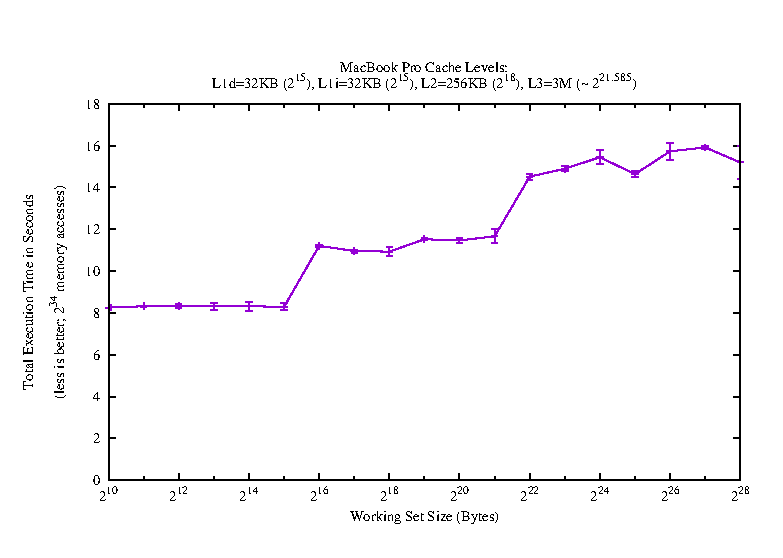
\includegraphics{appendix/plots-cache-measurements/plot-correct-ll}
\caption{Correct: Linked List, Sequential Access, and Single Loop}
\label{app:correct-ll-seqacc-sl}
\end{figure}

\begin{figure}[htbp]
\centering
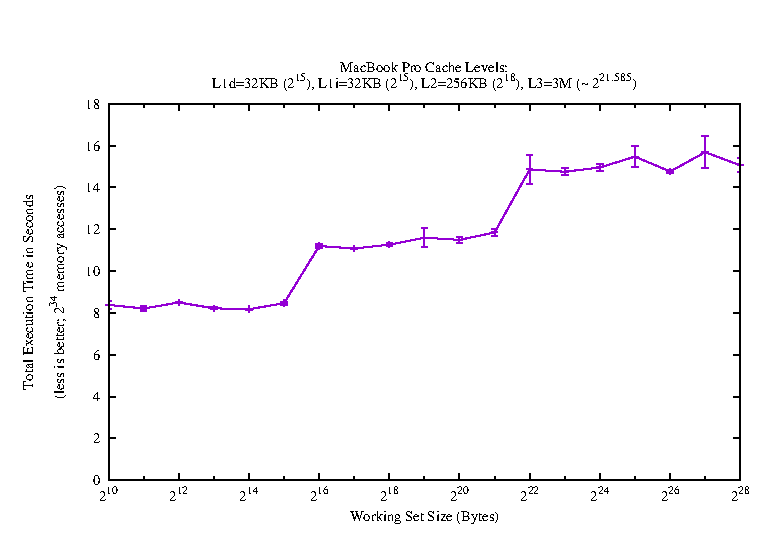
\includegraphics{appendix/plots-cache-measurements/plot-correct-array}
\caption{Correct: Array, Sequential Access, and Single Loop}
\label{app:correct-arr-seqacc-sl}
\end{figure}

\begin{figure}[htbp]
\centering
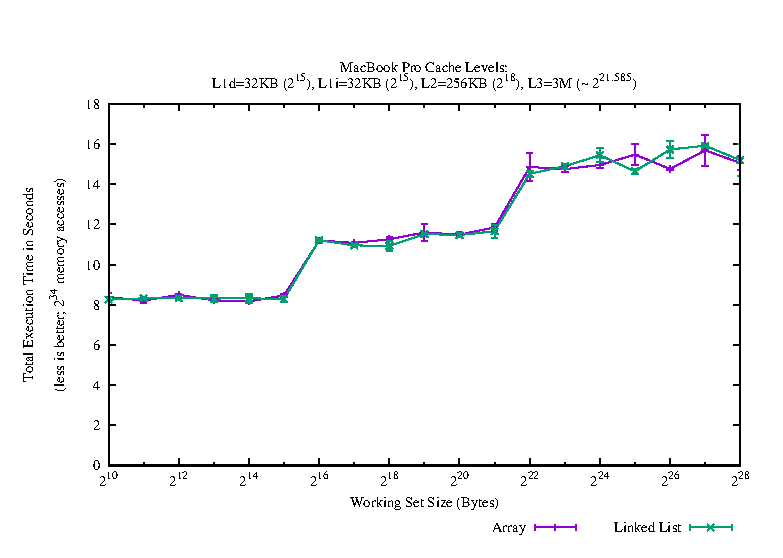
\includegraphics{appendix/plots-cache-measurements/plot-correct-array-ll}
\caption{Correct: Array, Sequential Access All, and Single Loop}
\label{app:correct-arr-seqaccall-sl}
\end{figure}

\hypertarget{big-iron9}{\subparagraph{\texorpdfstring{\texttt{big-iron9}}{big-iron9}}\label{big-iron9}}

So far all experiments are done on a MacBook pro. We re-run our approach
to solve the problem on \texttt{big-iron9} to corroborate our results.

The figure on the left shows the performance using a linked list. As
expected it illustrates nicely the cache hierarchy. We observe a
significant performance decrease at a working set size of 214 which
indicates at we now working on L2. There is another decrease around 220
which shows that L2 is not enough anymore and our data is stored in L3.
Take a look at a working set size of 224 presents the last decease of
performance, now our data is stored at the main memory.

The figure on the right shows the performance using an array. Obviously,
this approach offers better performance. This is different from the
execution on the MacBook, where performance for both approaches is quite
similar. Nevertheless, the shape of this figure presents the cache
hierarchy. We are able to observe which cache level is accessed for
which working set size. Even if the difference between L1 and L2 is very
small.

The third figure illustrates the differences of array and linked list.

\begin{figure}[htbp]
\centering
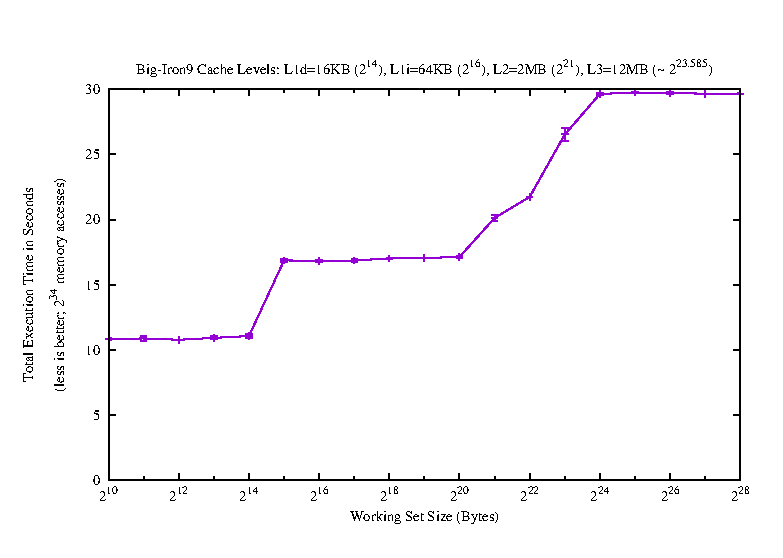
\includegraphics{appendix/plots-cache-measurements/plot-bi9-correct-ll}
\caption{Correct: Linked List, Sequential Access, and Single Loop}
\label{app:correct-ll-seqacc-sl-bi9}
\end{figure}

\begin{figure}[htbp]
\centering
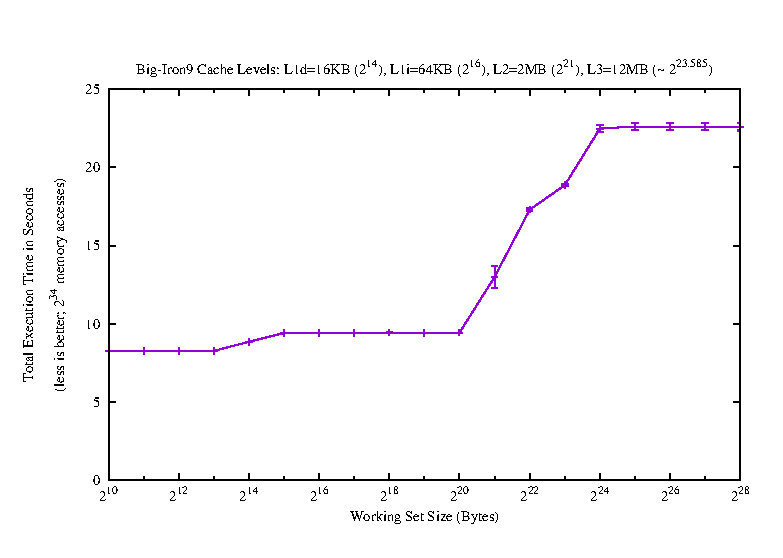
\includegraphics{appendix/plots-cache-measurements/plot-bi9-correct-array}
\caption{Correct: Array, Sequential Access, and Single Loop}
\label{app:correct-arr-seqacc-sl-bi9}
\end{figure}

\begin{figure}[htbp]
\centering
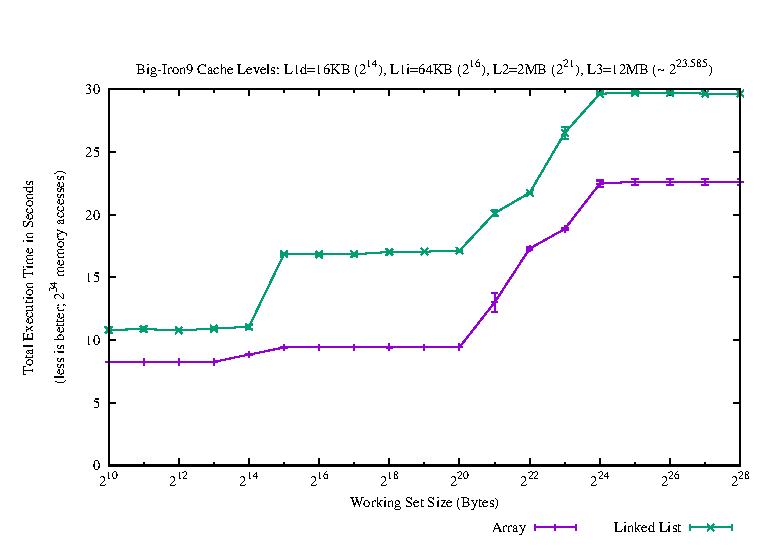
\includegraphics{appendix/plots-cache-measurements/plot-bi9-correct-array-ll}
\caption{Correct: Array, Sequential Access All, and Single Loop}
\label{app:correct-arr-seqaccall-sl-bi9}
\end{figure}

\subsection{Conclusion}\label{conclusion-5}

We started this report with experiments on different access methods of
our data structures linked list, and array, respectively. These
experiments nicely present performance differences. Furthermore, we
observe some interesting behavior for the array experiments. We define
this unexpected behavior as a problem and investigate it to find the
cause. Our investigations lead deeply into the generated assembly code.
We identified two reasons: (1) There is a special assembly command on
Intel x86 machines (\texttt{lea}) designed for array access without an
expensive memory access . (2) There are no assembly commands generated
for \texttt{C} code like \texttt{(void)cur-\textgreater{}pad{[}0{]};} if
there is no assignment. The combination of these leads to the working
set size independent performance of our array experiments. Finally, we
present a solution for this problem. Furthermore, we present experiments
which confirm the correctness of our solution.


%%%%%%%%%%%%%%%%%%%%%%%%%%%%%%%%%%%%%%%%
% List of figures/tables
\clearpage%
\listoffigures%
%
\clearpage%
\listoftables%
%
% \clearpage%
% \listofalgorithms%
%
%%%%%%%%%%%%%%%%%%%%%%%%%%%%%%%%%%%%%%%%
% Acronyms
%
\chapter{Acronyms}%
%
\begin{acronym}%
  \acro{CPA}{cycles per access}
  \acro{CPU}{central processing unit}
  \acro{LRU}{least recently used}
  \acro{trace}{memory access trace}
  \acro{MIN}{\Citeauthor{belady1966study}s algorithm}
\end{acronym}%
%
%%%%%%%%%%%%%%%%%%%%%%%%%%%%%%%%%%%%%%%
% Bibliography
%
\bibliographystyle{plainnat}%
\bibliography{references}%
%

\end{document}



















\chapter{Introduction}
\section{Definitions - V1}
\subsection{General definitions}
\begin{definition}[Command]
A command is an instruction with the purpose to perform some specific action, e.g, to add two numbers.
\end{definition}

\begin{definition}[Data]
Data is the information required by a program for its execution, e.g., values for computations.
\end{definition}

\begin{definition}[Program]
A program consists of a sequence of commands which operate on the programs data.
\end{definition}

\begin{definition}[CPU]
The CPU (central processing unit) executes a program, i.e., command by command is processed.
\end{definition}

\begin{definition}[Main Memory (in short: memory)]
Main Memory is a physical storage. It is structured in chunks of same size. During execution of a program the main memory stores the programs data and the program itself.
\end{definition}

\begin{definition}[Address]
A physical address is an unique identifier of a single memory chunk.
\end{definition}

%  chunk             address
%  M +-------------+ m
%    &     ...     |
%    &     ...     |
%    &     ...     |
%  J +-------------+ j
%    &    Data     |
%    + - - - - - - +
%    &   Program   |
%  I +-------------+ i
%    &     ...     |
%    &     ...     |
%    &     ...     |
%  0 +-------------+ 0

\begin{definition}[Allocator]
An allocator maintains a specific part of a programs data, the so-called \textit{heap}. The purpose of an allocator is to keep track about the addresses which are currently in use by the program (\textit{allocated}) and which are not (\textit{free}).
\end{definition}

%  M +-------------+     /  J +-------------+ address j
%    &     ...     &    /     &    Stack    |
%    &     ...     &   /      + ~ ~ ~ ~ ~ ~ + (*)
%    &     ...     &  /       & Free memory |
%  J +-------------+          + ~ ~ ~ ~ ~ ~ + (*)
%    &    Data     &          &             |
%  K + - - - - - - +          &    Heap     |
%    &   Program   &          &             |
%  I +-------------+          +-------------+
%    &     ...     &  \       &  Constants  |
%    &     ...     &   \    K + - - - - - - +
%    &     ...     &    \     &   Program   |
%  0 +-------------+     \  I +-------------+ address i
%  (*) Dynamic bound: Grows and shrinks during program execution.

\begin{definition}[Memory layout]
A memory layout describes which data is stored at which address. The memory layout is determined by the allocator.
\end{definition}

\begin{example}
Following example shows two possible memory layouts for the \texttt{data 0-10}. 
%  J +-------------+ j   /  + ~ ~ ~ ~ ~ ~ +  + ~ ~ ~ ~ ~ ~ +
%    &    Stack    &    /   &   data 00   &  &   data 10   &  address (k + 10)
%    + ~ ~ ~ ~ ~ ~ +   /    &   data 01   &  &   data 09   &  address (k + 9)
%    & Free memory &  /     &   data 02   &  &   data 08   &  address (k + 8)
%    + ~ ~ ~ ~ ~ ~ +        &   data 03   &  &   data 07   &  address (k + 7)
%    &             &        &   data 04   &  &   data 06   &  address (k + 6)
%    &    Heap     &        &   data 05   &  &   data 05   &  address (k + 5)
%    &             &        &   data 06   &  &   data 04   &  address (k + 4)
%  K +-------------+ k      &   data 07   &  &   data 03   &  address (k + 3)
%    &  Constants  &  \     &   data 08   &  &   data 02   &  address (k + 2)
%    + - - - - - - +   \    &   data 09   &  &   data 01   &  address (k + 1)
%    &   Program   &    \   &   data 10   &  &   data 00   &  address (k + 0)
%  I +-------------+ i   \  +-------------+  +-------------+
\end{example}

\begin{definition}[Register]
A register is a unit of memory directly accessed by the CPU. The CPU disposes over a limited number of register to process the commands of a program. Registers store commands, addresses of data or data.
\end{definition}

%  +---------------------+   +----------------------+ 
%  & Processor           &   & Memory               |
%  & +-----+-----------+ &   & +-----------+------+ |
%  & | CPU & Registers & <---> & Addresses & Data & |
%  & +-----+-----------+ &   & +-----------+------+ |
%  +---------------------+   +----------------------+

\begin{definition}[Data access]
A data access is a command aiming on processing data of a program. 
There are two \textit{access types}:
1. \textit{read} data: load the value stored at an address into a register
2. \textit{write} data: store the value of a register at an address

In general a data access consists of 3 components: (1) an access type, (2) an address, and (3) a register. For our purpose we don't care about the register. Hence, a data access is a tuple $(t, a)$ where $t$ is an access type and $a$ is an address (within the bounds of the program).
\end{definition}

\begin{definition}[Data access time]
The data access time is the amount of time it takes to data between a register and memory or vice versa.
\end{definition}

\begin{definition}[Trace]
The trace $T$ of a program $P$ is the sequence of data accesses $((t_0, a_0), (t_1, a_1), .. (t_{N-1}, a_{N-1}))$ of $P$, with $N > 0$ and $N =|T| \leq |P|$.
\end{definition}

\begin{definition}[Liveness interval of an address]
Assume a trace $T$ which contains an address $a$. The liveness interval of $a$ begins with the first data access on $a$ and ends with the last data access on $a$.

Assume tuple $(i,j)_a$ represents the liveness interval of an address $a$ of a trace $T$, $a \in T$ with $|T| = N$ and $0 \leq i,k \leq j,l < N$, then 
 - $(t_i, a_i) \in T$ s.t. $\not\exists k < i: (t_k, a) \wedge a_i = a$, and
 - $(t_j, a_j) \in T$ s.t. $\not\exists l > j: (t_l, a) \wedge a_j = a$.
\end{definition}

\begin{definition}[Cache]
A cache is a buffer which stores data currently used by the CPU. To be more precise if there is a data access on an address, this address and its data is temporally store within the cache.
\end{definition}

\begin{quote}
\textit{Note:} Caches where introduced, because the offer a smaller data access time than main memory does. This is beneficial for the total execution time of a program.

%  +---------------------+ +---------------------------+ +----------------------+
%  & Processor           & & Cache                     & & Memory               |
%  & +-----+-----------+ & & +----------------+------+ & & +-----------+------+ |
%  & | CPU & Registers & <-> & Some Addresses & Data & <-> & Addresses & Data & |
%  & +-----+-----------+ & & +----------------+------+ & & +-----------+------+ |
%  +---------------------+ +---------------------------+ +----------------------+
\end{quote}

\begin{definition}[Cache hit]
If the CPU processes a data access on an address which is already stored in the cache, this is called a \textit{cache hit}.
\end{definition}

\begin{definition}[Cache miss]
If the CPU processes a data access on an address which is not yet stored in the cache, this is called a \textit{cache miss}.
\end{definition}

\begin{definition}[Eviction strategy]
In case of a cache miss it is required make space for the requested address and its data. The \textit{eviction strategy} decides which address is evicted from the cache, i.e., the data of this address is written back to main memory.
\end{definition}

\subsection{Performance}
\begin{definition}[Program performance]
The performance of a program is the time (milliseconds) it take the CPU to process all commands, this is called \textit{total execution time}.
\end{definition}

\begin{definition}[Allocator performance]
The performance of an allocator is the number of cache misses yield by a programs trace.
\end{definition}

\subsection{Definitions required to transform a trace $T$ into single-assignment form}
\begin{definition}[Variable]
A variable $v$ is a unique identifier of the single-assignment form. 
\end{definition}

\begin{definition}[Assignment of a variable]
Each time an data access $(t, a)$ occurs in $T$, where $t$ is a \textit{write} access a new variable $v$ is chosen to replace $a$ for this data access and all following data accesses which are of type \textit{read}. (If address $a$ of trace $T$ is written multiple times each time an new variable is used.)
\end{definition}

\begin{definition}[Static-single-assignment form (SSA)]
A program is in single-assignment form if every variable has exactly one assignment.
\end{definition}


\section{Definitions - V2}

\subsection{The Memory Hierarchy}

% +-----+ cache store  +-------+ memory store  +-------------+
% |     |------------->|       |-------------->|             |
% | CPU |              |  SPM  |               | Main Memory |
% |     |<-------------|       |<--------------|             |
% +-----+  cache load  +-------+  memory load  +-------------+

\subsubsection{About Access Times}

Wikipedia 'Cache hierarchy'\footnote{\url{https://en.wikipedia.org/wiki/Cache\_hierarchy\#Properties}} describes several properties of caches that influence cache behaviour and access times:
\begin{itemize}
  \item Banked (separation of data and instruction caches) vs unified
  \item Inclusion vs exclusion vs non-inclusive non-exclusive: Defines whether data of lower caches is duplicated in higher caches.
  \item Write through vs write back: Defines whether data is written immediately or on eviction
  \item Write allocate vs write no-allocate: Defines whether data is fetched from memory on a write miss or not.
\end{itemize}

What every programmer should know about memory\cite{drepper2007every} has these numbers for access times:

\begin{table}
  \centering
  \begin{tabular}[c]{|l|r|r|}
    \hline
    To Where & Cycles & Factor to lower memory \tabularnewline
    \hline \hline
    Register & $\leq$  1 &     - \tabularnewline
    L1d      &       \~3 &     3 \tabularnewline
    L2       &      \~14 &  4.67 \tabularnewline
    RAM      &     \~240 & 17.14 \tabularnewline
    \hline
  \end{tabular}
  \caption{\todo{add caption}}
  \label{tab:def-access-times-1}
\end{table}

The 7zip benchmark pages\footnote{\url{http://www.7-cpu.com/cpu/Skylake.html}} has cycle time numbers for modern processors. 
For example for a Intel i7-6700 (Skylake):

\begin{table}
  \centering
  \begin{tabular}[c]{|l|r|r|}
    \hline
    To Where & Latency & Factor to lower memory \tabularnewline
    \hline \hline
    L1d &                          4 or 5 cycles &  5.0 \tabularnewline
    L2  &                              12 cycles &  2.4 \tabularnewline
    L3  &                        38 or 42 cycles &  3.5 \tabularnewline
    RAM & 42 cycles + 51 ns (= 246 cycles @4GHz) & 5.86 \tabularnewline
  \end{tabular}
  \caption{\todo{add caption}}
  \label{tab:def-access-times-2}
\end{table}

\subsection{The Model}

\begin{definition}[trace]
A trace is a sequence of instructions.
\end{definition}

\begin{definition}[instruction]
An instruction is an access to an address given by the tupel $(t, a)$ with $t$ in ${Read, Write}$ and $a$ an address in main memory.
\end{definition}

\begin{definition}[Address]
A location in the memory that one variable can occupy for a certain period of time.
\end{definition}

\begin{definition}[Variable]
A value that can change overtime. In this context, a variable is a name that represents a data used by the trace. it can change according to the trace transformations.
\end{definition}

\begin{definition}[Single assignment form (SA)]
A trace is in single assignment form if every variable has exactly one assignment. \cite{rosen1988global} \cite{alpern1988detecting}
\end{definition}


\begin{definition}[Trace transformation]
Trace transformation
\end{definition}

\begin{definition}[Initial trace]
The initial trace $T$ of a program $P$ is the sequence of 'data' accesses $((t_0, a_0), (t_1, a_1), \dots (t_{N-1}, a_{N-1}))$ of $P$, with $N > 0$ and $N = |T| \leq |P|$.
\end{definition}

\begin{definition}[Data]
A data is an information processed or stored by a computer.
\end{definition}

\begin{definition}[Variable]
A variable $v$ is a unique identifier of the single-assignment form.
\end{definition}

\begin{definition}[Assignment of a variable]
Each time an data access $(t, a)$ occurs in $T$, where $t$ is a \textit{write} access a new variable $v$ is chosen to replace $a$ for this data access and all following data accesses which are of type \textit{read}. (If address $a$ of trace $T$ is written multiple times each time an new variable is used.)
\end{definition}

\begin{definition}[Canonical Form]
A canonical form trace is the trace obtained after the single Assignment transformation.
\end{definition}

\begin{definition}[Liveness interval of a variable]
The liveness interval of a variable is the continuous period of time where the variable is occupying an addresse. (the change of the addresse occupied implies a new liveness interval / "continous" means no other variable was placed in this address during this time period).
\end{definition}

% +------------+                                     +------------+
% | Trace file |                                     | Single     |
% |            | ----------------------------------> | Assignment |
% | (.trace)   |  Single Assignment Transformation   | Trace      |
% +------------+                                     +------------+

\begin{definition}[Allocator]
An allocator maintains a specific part of a programs data, the so-called \textit{heap}. The purpose of an allocator is to keep track about the addresses which are currently in use by the program (\textit{allocated}) and which are not (\textit{free}).
\end{definition}

\begin{definition}[Allocator Trace]
Allocator Trace
\end{definition}

\begin{definition}[Memory layout]
A memory layout describes which data is stored at which address. The memory layout is determined by the allocator.
\end{definition}

\begin{definition}[Address]
A location in the memory that one variable can occupy for a certain period of time.
\end{definition}

 %  chunk             address
 % M +-------------+ m
 %   |     ...     |
 %   |     ...     |
 %   |     ...     |
 % J +-------------+ j
 %   |    Data     |
 %   + - - - - - - +
 %   |   Program   |
 % I +-------------+ i
 %   |     ...     |
 %   |     ...     |
 %   |     ...     |
 % 0 +-------------+ 0

\begin{definition}[Physical Address]
A physical address is an unique identifier of a single memory chunk.
\end{definition}

\begin{definition}[Virtual Address]
A virtual address is an unique identifier of a physical address in the context of a program, i.e., there is only one virtual address 0 within a program but multiple programs might make use of an virtual address 0.
\end{definition}

\begin{definition}[Trace allocator]
The initial trace $T$ of a program $P$ is the sequence of 'addresses' accesses $((t_0, a_0), (t_1, a_1), \dots (t_{N-1}, a_{N-1}))$ of $P$, with $N > 0$ and $N = |T| \leq |P|$.
\end{definition}

\begin{definition}[Memory layout]
A memory layout describes which data is stored at which address. The memory layout is determined by the allocator.
\end{definition}

% +------------+   +-----------+   +-----------+
% | Single     |   |           |   | Allocator |
% | Assignment | + | Allocator | = | Trace     |
% | Trace      |   |           |   |           |
% +------------+   +-----------+   +-----------+

\begin{definition}[Memory Model]
Memory Model
\end{definition}

\begin{definition}[Performance]
Performance
\end{definition}

\begin{definition}[Cache]
A cache is a buffer which stores data currently used by the CPU. To be more precise if there is a data access on an address, this address and its data is temporally store within the cache.
\end{definition}

% +---------------------+ +---------------------------+ +----------------------+
% | Processor           | | Cache                     | | Memory               |
% | +-----+-----------+ | | +----------------+------+ | | +-----------+------+ |
% | | CPU | Registers | <-> | Some Addresses | Data | <-> | Addresses | Data | |
% | +-----+-----------+ | | +----------------+------+ | | +-----------+------+ |
% +---------------------+ +---------------------------+ +----------------------+

\begin{definition}[Address Spaces]
The address space is the set of addresses in the memory that will be used by the trace.
\end{definition}

\begin{definition}[Register]
A register is a unit of memory directly accessed by the CPU. The CPU disposes over a limited number of register to process the commands of a program. Registers store commands, addresses of data or data.
\end{definition}

% +---------------------+   +----------------------+
% | Processor           |   | Memory               |
% | +-----+-----------+ |   | +-----------+------+ |
% | | CPU | Registers | <---> | Addresses | Data | |
% | +-----+-----------+ |   | +-----------+------+ |
% +---------------------+   +----------------------+

\begin{definition}[Main Memory]
Main Memory is a physical storage. It is structured in chunks of same size. During execution of a program the main memory stores the programs data and the program itself.
\end{definition}

\begin{example}
Following example shows two possible memory layouts for the `data 0-10`.
% J +-------------+ j   /  + ~ ~ ~ ~ ~ ~ +  + ~ ~ ~ ~ ~ ~ +
%   |    Stack    |    /   |   data 00   |  |   data 10   |  address (k + 10)
%   + ~ ~ ~ ~ ~ ~ +   /    |   data 01   |  |   data 09   |  address (k + 9)
%   | Free memory |  /     |   data 02   |  |   data 08   |  address (k + 8)
%   + ~ ~ ~ ~ ~ ~ +        |   data 03   |  |   data 07   |  address (k + 7)
%   |             |        |   data 04   |  |   data 06   |  address (k + 6)
%   |    Heap     |        |   data 05   |  |   data 05   |  address (k + 5)
%   |             |        |   data 06   |  |   data 04   |  address (k + 4)
% K +-------------+ k      |   data 07   |  |   data 03   |  address (k + 3)
%   |  Constants  |  \     |   data 08   |  |   data 02   |  address (k + 2)
%   + - - - - - - +   \    |   data 09   |  |   data 01   |  address (k + 1)
%   |   Program   |    \   |   data 10   |  |   data 00   |  address (k + 0)
% I +-------------+ i   \  +-------------+  +-------------+
\end{example}

\begin{definition}[CPU]
The CPU (central processing unit) executes a program, i.e., command by command is processed.
\end{definition}

\begin{definition}[Data access]
A data access is a command aiming on processing data of a program. There are two \textit{access types}:
\begin{enumerate}
  \item \textit{read} data: load the value stored at an address into a register
  \item \textit{write} data: store the value of a register at an address
\end{enumerate}
In general a data access consists of 3 components: (1) an access type, (2) an address, and (3) a register. For our purpose we don't care about the register. Hence, a data access is a tuple $(t, a)$ where $t$ is an access type and $a$ is an address (within the bounds of the program).
\end{definition}

\begin{definition}[Data access time]
The data access time is the amount of time it takes to data between a register and memory or vice versa.
\end{definition}

\begin{definition}[Cache Hit]
If the CPU processes a data access on an address which is already stored in the cache, this is called a \textit{cache hit}.
\end{definition}

\begin{definition}[Cache Miss]
If the CPU processes a data access on an address which is not yet stored in the cache, this is called a \textit{cache miss}.
\end{definition}

\begin{definition}[Eviction strategy]
In case of a cache miss it is required make space for the requested address and its data. The \textit{eviction strategy} decides which address is evicted from the cache, i.e., the data of this address is written back to main memory.
\end{definition}

\subsection{Performance}
\begin{definition}[Program performance]
The performance of a program is the time it take the CPU to process all commands, this is called \textit{total execution time}
\end{definition}

\begin{definition}[Allocator performance]
The performance of an allocator is the number of cache misses yield by a programs trace.
\end{definition}

% +-----------+   +--------+
% | Allocator |   | Memory |
% | Trace     | + | Model  | = Performance metric
% |           |   |        |
% +-----------+   +--------+

\subsection{The Allocators}

\subsubsection{SingleAssignmentAllocator}
\subsubsection{IdentityAllocator}
\subsubsection{CompactStackAllocator}
\subsubsection{CompactQueueAllocator}
\subsubsection{CompactRandomAllocator}

\subsection{The Caches}
\subsubsection{BeladyCache}
\subsubsection{OPTCache}
\subsubsection{ValgrindCache}
\subsubsection{ValgrindLivenessCache}

%%%%%%%%%%%%%%%%%%%%%%%%%%%%%%%%%%%%%%%%%%%%%%%%%%%%%%%%%%%%%%%%%%%%%%%%%%%%%%%%%%%%%%%%%%%%%%%%%%%
%%%%%%%%%%%%%%%%%%%%%%%%%%%%%%%%%%%%%%%%%%%%%%%%%%%%%%%%%%%%%%%%%%%%%%%%%%%%%%%%%%%%%%%%%%%%%%%%%%%
%%%%%%%%%%%%%%%%%%%%%%%%%%%%%%%%%%%%%%%%%%%%%%%%%%%%%%%%%%%%%%%%%%%%%%%%%%%%%%%%%%%%%%%%%%%%%%%%%%%
%%%%%%%%%%%%%%%%%%%%%%%%%%%%%%%%%%%%%%%%%%%%%%%%%%%%%%%%%%%%%%%%%%%%%%%%%%%%%%%%%%%%%%%%%%%%%%%%%%%


\chapter{Experiments}

\section{Compact Allocators}

\begin{quote}
For a given trace, can I get a better (the optimal) performance simply by changing addresses?
\end{quote}

\subsection{Previous Work}

The last reports have shown that in the context of scratchpad memory and with full knowledge about the liveness of addresses the number of memory accesses is independent of the memory layout. The number of misses, however, is influenced by it.
The plots suggest that a compacting allocator which reuses cached dead items gives a transformation that is minimal in the number of misses when using a scratchpad memory model.

\begin{quote}
Given a trace $T$, liveness information of addresses of $T$, a scratchpad memory and a scratchpad strategy based on $T$. Then, a compacting allocator that reuses cached dead items when possible gives the transformed trace $T'$ that is optimal in the number of misses.
\end{quote}

This report compares several implementations of compacting allocators.

\subsection{Methodology}

We compare the following allocators.
\begin{enumerate}
  \item \textbf{Identity} Addresses are unchanged from the identity \ac{trace}.
  \item \textbf{SSA} Addresses are not reused.
  \item \textbf{CompactStack} Bump pointer allocator with a free list with stack semantics. Freed addresses are appended at the end and popped from the end on allocation.
  \item \textbf{CompactQueue} Bump pointer allocator with a free list with queue semantics. Freed addresses are appended at the end and taken from the beginning on allocation.
  \item \textbf{CompactRandom} Bump pointer allocator with a free list where free addresses are chosen at random on allocation.
  \item \textbf{CompactCached} Bump pointer allocator that reuses a freed, cached address if there is one or a stack-like free list otherwise.
\end{enumerate}

The memory model is again a scratchpad memory with 8-byte lines and an increasing size.

Again, the results for the V8 benchmarks Richards, Deltablue, and Raytrace are plotted.

\subsection{Results}

\subsubsection{Richards - misses}
\begin{table}
  \centering
  \begin{tabular}[c]{|l|r|r|r|r|r|r|}
    \hline
    \textbf{SPM size in bytes} & \textbf{Identity} & \textbf{SSA} & \textbf{CompactStack} & \textbf{CompactQueue} & \textbf{CompactRandom} & \textbf{CompactCached} \tabularnewline
    \hline \hline
    1024  & 19906406 & 27186015 & 14288773 & 27185933 & 14659129 & 13501287 \tabularnewline   
    2048  & 13348365 & 21797929 &  7037009 & 21797723 &  7436173 &  6334160 \tabularnewline  
    4096  &  8502161 & 19039748 &  2529214 & 19038965 &  3015836 &  2094777 \tabularnewline  
    8192  &  5997722 & 18550483 &  1587408 & 18548641 &  2135818 &  1263075 \tabularnewline  
    16384 &  5278238 & 18315329 &  1128682 & 18305995 &  1707261 &   859009 \tabularnewline 
    32768 &  5077416 & 18178226 &   857012 & 18080705 &  1449062 &   618508 \tabularnewline 
    65536 &  4495702 & 18094113 &   677410 & 17684018 &  1262799 &   466934 \tabularnewline
    \hline
  \end{tabular}
  \caption{\todo{add caption}}
  \label{tab:experiment-compact-richards-misses}
\end{table}

\begin{figure}[ht]
  \centering
  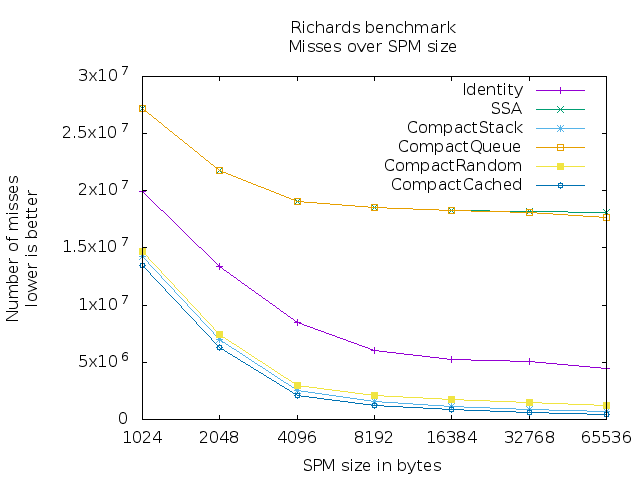
\includegraphics[width = .75\textwidth]{plots/compact-richards.png}
  \caption{Misses of Richards benchmark}
  \label{fig:experiment-compact-richards-misses}
\end{figure}

\subsubsection{DeltaBlue - misses}

\begin{table}
  \centering
  \begin{tabular}[c]{|l|r|r|r|r|r|r|}
    \hline
    \textbf{SPM size in bytes} & \textbf{Identity} & \textbf{SSA} & \textbf{CompactStack} & \textbf{CompactQueue} & \textbf{CompactRandom} & \textbf{CompactCached} \tabularnewline
    \hline \hline
    1024  & 77146231 & 98768459 & 52700195 & 98768383 & 53306777 & 50758432 \tabularnewline
    2048  & 53120872 & 79005685 & 28072125 & 79005479 & 28715840 & 25892998 \tabularnewline
    4096  & 41637998 & 70953742 & 16673778 & 70952971 & 17370985 & 14835627 \tabularnewline
    8192  & 28707195 & 65036775 &  7392572 & 65035091 &  8198850 &  6270975 \tabularnewline
    16384 & 23906668 & 62731219 &  3346997 & 62714931 &  4278582 &  2612975 \tabularnewline
    32768 & 20440744 & 62151273 &  2151620 & 62022996 &  3109816 &  1576686 \tabularnewline
    65536 & 20079036 & 61858627 &  1516174 & 61517639 &  2497068 &  1043268 \tabularnewline
    \hline
  \end{tabular}
  \caption{\todo{add caption}}
  \label{tab:experiment-compact-deltablue-misses}
\end{table}

\begin{figure}[ht]
  \centering
  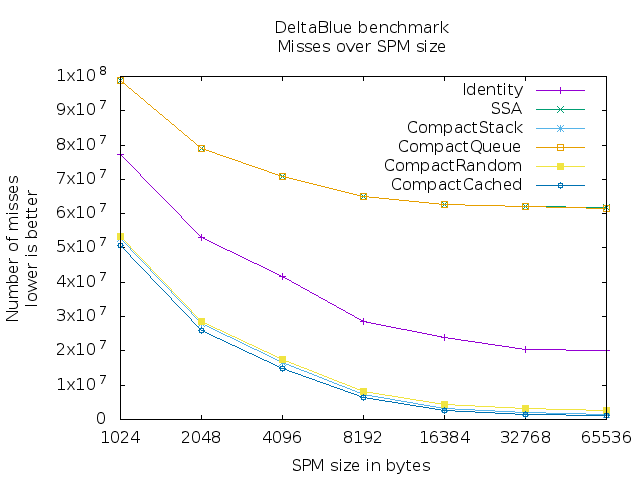
\includegraphics[width = .75\textwidth]{plots/compact-deltablue.png}
  \caption{Misses of DeltaBlue benchmark}
  \label{fig:experiment-compact-deltablue-misses}
\end{figure}

\subsubsection{Raytrace - misses}

\begin{table}
  \centering
  \begin{tabular}[c]{|l|r|r|r|r|r|r|}
    \hline
    \textbf{SPM size in bytes} & \textbf{Identity} & \textbf{SSA} & \textbf{CompactStack} & \textbf{CompactQueue} & \textbf{CompactRandom} & \textbf{CompactCached} \tabularnewline
    \hline \hline
    1024  & 17020972 & 24944756 & 11379998 & 24944674 & 11800338 & 10296539 \tabularnewline
    2048  & 14440844 & 23046938 &  8474762 & 23046732 &  8923334 &  7499105 \tabularnewline
    4096  & 12541349 & 21674551 &  6328499 & 21673768 &  6803800 &  5444919 \tabularnewline
    8192  & 10856047 & 20607354 &  4517425 & 20605669 &  5020860 &  3757431 \tabularnewline
    16384 &  9491867 & 19882091 &  3159250 & 19876330 &  3705843 &  2531928 \tabularnewline
    32768 &  8906151 & 19497833 &  2429807 & 19478760 &  2996836 &  1877661 \tabularnewline
    65536 &  8218054 & 19236973 &  1910619 & 19173814 &  2483494 &  1421185 \tabularnewline
    \hline
  \end{tabular}
  \caption{\todo{add caption}}
  \label{tab:experiment-compact-raytrace-misses}
\end{table}

\begin{figure}[ht]
  \centering
  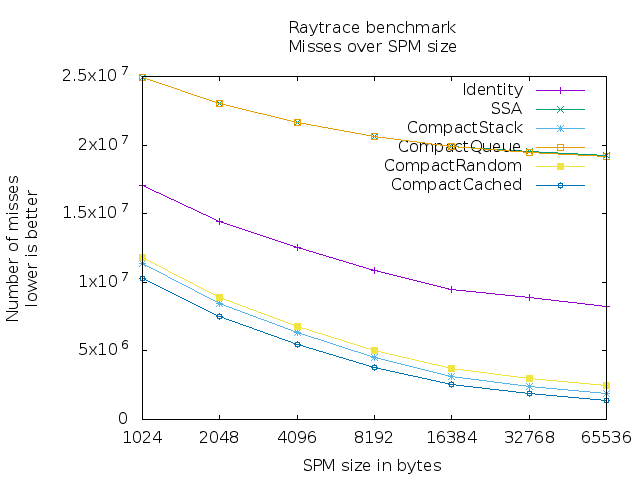
\includegraphics[width = .75\textwidth]{plots/compact-raytrace.png}
  \caption{Misses of Raytrace benchmark}
  \label{fig:experiment-compact-raytrace-misses}
\end{figure}

\subsubsection{Navier-Stokes - misses}

From Chromium Blog\footnote{\url{https://blog.chromium.org/2012/03/v8-benchmark-suite-extended-with.html}}
\begin{quote}
  This new version adds Oliver Hunt's 2D Navier-Stokes fluid dynamic simulation, which stresses intense double array computations. These complex double array computations are today common in games, graphic and scientific applications.
\end{quote}

\begin{table}
  \centering
  \begin{tabular}[c]{|l|r|r|r|r|r|r|}
    \hline
    \textbf{SPM size in bytes} & \textbf{Identity} & \textbf{SSA} & \textbf{CompactStack} & \textbf{CompactQueue} & \textbf{CompactRandom} & \textbf{CompactCached} \tabularnewline
    \hline \hline
    1024  & 151591543 & 197638846 & 122279178 & 197638770 & 124040970 & 120281818 \tabularnewline
    2048  & 126350972 & 173010778 &  96389043 & 173010573 &  98196415 &  94309498 \tabularnewline
    4096  & 123796035 & 170945407 &  93487986 & 170944635 &  95316020 &  91414571 \tabularnewline
    8192  & 121982315 & 169615053 &  91176334 & 169613376 &  93022611 &  89148010 \tabularnewline
    16384 & 118622912 & 167610304 &  87596431 & 167604544 &  89467888 &  85647336 \tabularnewline
    32768 & 114717104 & 163980384 &  81473478 & 163960984 &  83360157 &  79583462 \tabularnewline
    65536 & 106277710 & 156998071 &  70413666 & 156881332 &  72288424 &  68566643 \tabularnewline
    \hline
  \end{tabular}
  \caption{\todo{add caption}}
  \label{tab:experiment-compact-navier-stokes-misses}
\end{table}

\begin{figure}[ht]
  \centering
  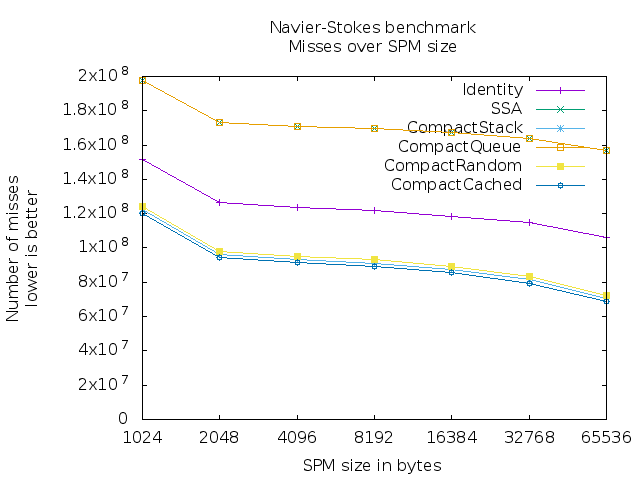
\includegraphics[width = .75\textwidth]{plots/compact-navier-stokes.png}
  \caption{Misses of Navier-Stokes benchmark}
  \label{fig:experiment-compact-navier-stokes-misses}
\end{figure}

\subsection{Conclusion}

The plots show that CompactCached has the fewest misses of all implemented compacting allocators.
Also, CompactStack has a comparable number of misses.
Interestingly also CompactRandom comes close.
We will examine if this is because of a flawed implementation or actual legit behavior.

While the plots suggest that CompactCached is better than any other examined allocator we still need solid evidence for this property.


\section{8th June, 2017 and 13th June, 2017}
\begin{quote}[Research question]
Can I get the optimal performance by changing the addresses used by a given trace $T$?
\end{quote}

\subsection{What is this report about?}
The purpose of this experiment is to show that under certain assumptions the memory layout has no impact on the number of memory accesses.

\subsection{Experimental setup}
\subsubsection{Definitions}

\begin{definition}[Instruction] 
An instruction is the pair $(t, a)$ where $t \in {R, W}$ denotes read and write access and $a$ the address being accessed.
\end{definition}

\begin{definition}[Trace] 
A trace is a sequence $((t_0, a_0), (t_1, a_1), ..., (t_{n-1}, a_{n-1}))$ of pairs with $0 \leq i < n$ where $t_i \in {R, W}$ denotes read or write access and $a_i$ the address being accessed.
\end{definition}

\begin{definition}[Liveness interval] 
A liveness interval is defined as the interval between a write to an address and the final access before the next write to the same address or the end of the trace.
\end{definition}

\begin{definition}[Trace transformation] 
We define a transformation between traces $T$ and $T'$ as a renaming of addresses such that liveness intervals are unchanged.
\end{definition}

\begin{definition}[Scratchpad memory (SPM)] 
A scratchpad memory is an application controlled, fast memory. A subset of addresses in main memory.
\end{definition}

% +-----+ store  +-------+ store  +-----+
% &     |------->|       |------->|     |
% & CPU &        &  SPM  &        & RAM |
% &     |<-------|       |<-------|     |
% +-----+  load  +-------+  load  +-----+

\begin{definition}[Memory accesses] 
A store or a load between scratchpad memory and main memory.
\end{definition}

\begin{definition}[Miss] 
Whenever the accesses item is not in the SPM it is a \textit{miss}, other wise it is a \textit{hit}.
\end{definition}

\begin{definition}[Performance] 
Performance is defined as the number of memory accesses during the the execution of a trace $T$.
\end{definition}

\begin{definition}[Optimal Performance] 
The optimal performance is the minimal number of memory accesses of all possible transformations of a trace $T$.
\end{definition}

\begin{definition}[The minimum heap size] 
Let $n_i$ $0 \leq i \leq N$ be the numbers of overlapping intervals at instruction $i$ of the trace. The minimum heap size is: $n_max * word_size$ where $n_max = \max{n_i, 0 \leq i \leq N}$.
\end{definition}

\subsection{Hypothesis}

Given a trace $T$, a scratchpad memory, liveness intervals of $T$, then the number of memory accesses is constant for any memory layout.

\subsection{Experiments}

The tiny experiment is repeated on traces of V8 benchmarks for an SPM size of $2^10$ bytes to $2^16$ bytes. Shown in this table is the number of memory accesses for each allocator as well as the average and standard deviation across all allocators.

Benchmark description taken from Chromium Blog (\url{https://blog.chromium.org/2010/10/v8-benchmark-suite-updated.html}).

\subsubsection{Tiny Example}

Take an example trace (all accesses are 8 bytes):

\begin{lstlisting}
0: W 8
1: W 16
2: W 24
3: R 16
4: R 8
5: W 32
6: R 24
7: R 32
8: R 24
9: R 16
\end{lstlisting}

We compute the misses and memory accesses of four allocators (= trace transformations):
\begin{enumerate}
\item \textbf{Identity:} Addresses are unchanged
\item \textbf{Compact:} Bump pointer allocator with a free stack
\item \textbf{Random:} Random addresses
\item \textbf{SSA:} Bump pointer without reusing of addresses
\end{enumerate}

The SPM has a size of 16 bytes and lines of 8 bytes.

Let us look at a few situations:
\begin{enumerate}
\item At instruction 2 there is a write access to address 24, the SPM contains 8 and 16. Both items in SPM are live. The item which access is the furthest in the future is chosen to be stored to main memory and replaced by the new item (see Belady's algorithm \cite{belady1966study}). This is 8 in this case. Since the new item is written to there is no need to load its content from main memory. This instruction therefore results in 1 memory access.
\item At instruction 4 there is a read request to address 8, the SPM contains 16 and 24. According to Belady 16 is selected for eviction and stored to main memory. The new item is read, therefore its content has to be loaded from main memory. This instruction results in 2 memory access.
\item At instruction 9 the address 16 is read. Both items in the SPM are dead, therefore they do not have to stored back to main memory for eviction. Regardless of the eviction choice, only the read item has to be loaded from main memory, resulting in 1 memory access for this instruction.
\end{enumerate}

The experiment is run with \texttt{semloc} and these parameters:

\begin{lstlisting}
bin/semloc -c 4 -C 4 -l 8 -L 8 -a 3 -A 3 traces/spm-example.trace 
\end{lstlisting}

The results are

\begin{table}
  \centering
  \begin{tabular}[c]{|l|c|c|}
    \hline
    \textbf{Allocator} & \textbf{Misses} & \textbf{Memory Accesses} \tabularnewline
    \hline\hline
    Identity & 6 & 4 \tabularnewline
    Compact  & 5 & 4 \tabularnewline
    Random   & 6 & 4 \tabularnewline
    SSA      & 6 & 4 \tabularnewline
    \hline
  \end{tabular}
  \caption{\todo{add caption}}
  \label{tab:experiment-2017-june-8}
\end{table}

The trace results in 4 memory access for all allocators. This suggests that memory accesses in the context of SPM are indeed independent of memory layout.

The Compact allocator has 5 misses, as opposed to all other which have 6 misses: At instruction 5 the new address 32 is written to. At this point, address 8 is dead and in the SPM. The Compact allocator reuses address 8, thus resulting in a hit. Other allocators do not exploit this possibility and have a miss at this instruction.

% \subsection{Conclusion}
% We presented the hypothesis that the memory layout does not matter for scratchpad memories, which know the trace T and liveness intervals of T. For illustrations we discussed a small example which confirms our hypothesis.

% In our example the Belady eviction policy in combination with liveness intervals make sure that memory accesses and misses remain minimal. The compact allocator only has a chance to get below that number of misses, because it turns a miss into a hit. At allocation time he can immediately achieve this by reusing a dead address in SPM.

% To conclude, this small example nicely illustrations that for systems which has certain information about there applications the memory layout has no influence.


\subsubsection{V8 benchmark: Richards}

Operating system kernel simulation benchmark originally written in BCPL by Martin Richards. The Richards benchmark effectively measures how fast the JavaScript engine is at accessing object properties, calling functions, and dealing with polymorphism. It is a standard benchmark that has been successfully used to measure the performance of many modern programming language implementations.

Trace size: 83M instructions

Memory accesses:
\begin{table}
  \centering
  \begin{tabular}[c]{|l|r|r|r|r|r|r|}
    \hline
    \textbf{SPM size in bytes} & \textbf{Identity} & \textbf{Compact} & \textbf{Random} & \textbf{SSA} & \textbf{Average} \tabularnewline
    \hline \hline
    1024  & 18654262 & 18654262 & 18654262 & 18654262 & 18654262 \tabularnewline
    2048  &  7878090 &  7878090 &  7878090 &  7878090 &  7878090 \tabularnewline
    4096  &  2361728 &  2361728 &  2361728 &  2361728 &  2361728 \tabularnewline
    8192  &  1383198 &  1383198 &  1383198 &  1383198 &  1383198 \tabularnewline
    16384 &   912890 &   912890 &   912890 &   912890 &   912890 \tabularnewline
    32768 &   638684 &   638684 &   638684 &   638684 &   638684 \tabularnewline
    65536 &   470458 &   470458 &   470458 &   470458 &   470458 \tabularnewline
    \hline
  \end{tabular}
  \caption{\todo{add caption}}
  \label{tab:experiment-2017-june-8-richards-mem}
\end{table}


Misses:
\begin{table}
  \centering
  \begin{tabular}[c]{|l|r|r|r|r|}
    \hline
    \textbf{SPM size in bytes} & \textbf{Identity} & \textbf{Compact} & \textbf{Random} & \textbf{SSA}  \tabularnewline
    \hline \hline
    1024  & 19906406 & 14288773 & 27186015 & 27186015 \tabularnewline
    2048  & 13348365 &  7037009 & 21797929 & 21797929 \tabularnewline
    4096  &  8502161 &  2529214 & 19039748 & 19039748 \tabularnewline
    8192  &  5997722 &  1587408 & 18550483 & 18550483 \tabularnewline
    16384 &  5278242 &  1128682 & 18315329 & 18315329 \tabularnewline
    32768 &  5077416 &   857012 & 18178226 & 18178226 \tabularnewline
    65536 &  4495702 &   677410 & 18094113 & 18094113 \tabularnewline
    \hline
  \end{tabular}
  \caption{\todo{add caption}}
  \label{tab:experiment-2017-june-8-richards-misses}
\end{table}

\begin{figure}[ht]
  \centering
  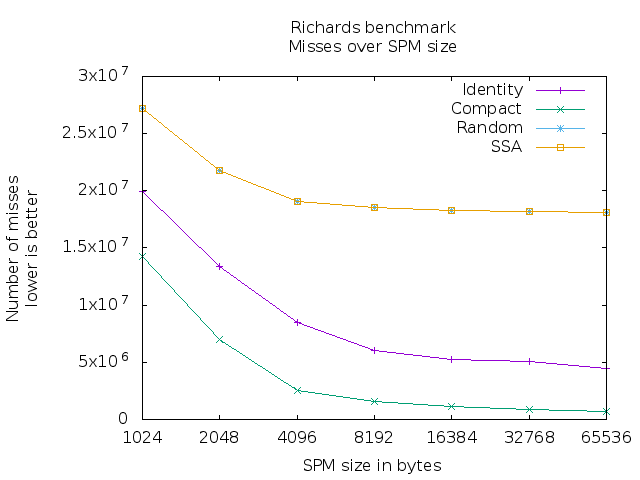
\includegraphics[width = .75\textwidth]{plots/2017-06-13-richards-misses.png}
  \caption{Misses of Richards benchmark}
  \label{fig:experiment-2017-june-8-richards-misses}
\end{figure}

\subsubsection{V8 benchmark: Deltablue}

>One-way constraint solver, originally written in Smalltalk by John Maloney and Mario Wolczko. The DeltaBlue benchmark is written in an object-oriented style with a multi-level class hierarchy. As such it measures how fast the JavaScript engine is at running well-structured applications with many objects and small functions.

Trace size: 272M instructions

Memory accesses:
\begin{table}
  \centering
  \begin{tabular}[c]{|l|r|r|r|r|r|r|}
    \hline
    \textbf{SPM size in bytes} & \textbf{Identity} & \textbf{Compact} & \textbf{Random} & \textbf{SSA} & \textbf{Average} \tabularnewline
    \hline \hline
    1024  & 74897566 & 74897566 & 74897566 & 74897566 & 74897566 \tabularnewline
    2048  & 35372018 & 35372018 & 35372018 & 35372018 & 35372018 \tabularnewline
    4096  & 19268132 & 19268132 & 19268132 & 19268132 & 19268132 \tabularnewline
    8192  &  7434198 &  7434198 &  7434198 &  7434198 &  7434198 \tabularnewline
    16384 &  2823086 &  2823086 &  2823086 &  2823086 &  2823086 \tabularnewline
    32768 &  1663194 &  1663194 &  1663194 &  1663194 &  1663194 \tabularnewline
    65536 &  1077902 &  1077902 &  1077902 &  1077902 &  1077902 \tabularnewline
    \hline
  \end{tabular}
  \caption{\todo{add caption}}
  \label{tab:experiment-2017-june-8-deltablue-mem}
\end{table}

Misses:
\begin{table}
  \centering
  \begin{tabular}[c]{|l|r|r|r|r|}
    \hline
    \textbf{SPM size in bytes} & \textbf{Identity} & \textbf{Compact} & \textbf{Random} & \textbf{SSA}  \tabularnewline
    \hline \hline
    1024  & 77146231 & 52700195 & 98768459 & 98768459 \tabularnewline
    2048  & 53120872 & 28072125 & 79005685 & 79005685 \tabularnewline
    4096  & 41637998 & 16673778 & 70953742 & 70953742 \tabularnewline
    8192  & 28707195 &  7392572 & 65036775 & 65036775 \tabularnewline
    16384 & 23906672 &  3346997 & 62731219 & 62731219 \tabularnewline
    32768 & 20440744 &  2151620 & 62151273 & 62151273 \tabularnewline
    65536 & 20079036 &  1516174 & 61858627 & 61858627 \tabularnewline
    \hline
  \end{tabular}
  \caption{\todo{add caption}}
  \label{tab:experiment-2017-june-8-deltablue-misses}
\end{table}

\begin{figure}[ht]
  \centering
  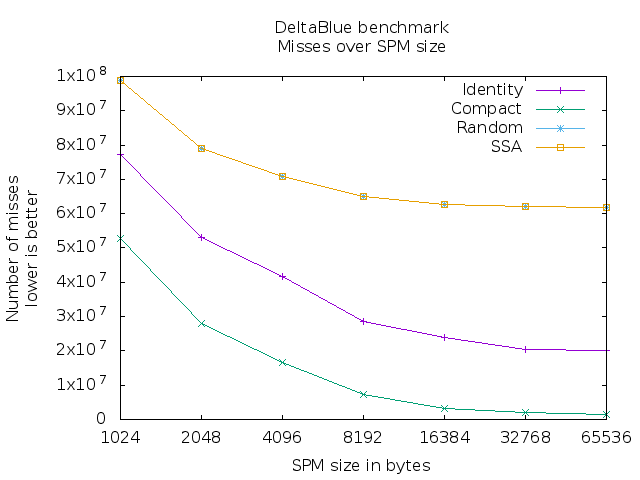
\includegraphics[width = .75\textwidth]{plots/2017-06-13-deltablue-misses.png}
  \caption{Misses of Deltablue benchmark}
  \label{fig:experiment-2017-june-8-deltablue-misses}
\end{figure}

\subsubsection{V8 benchmark: Raytrace}

Ray tracer benchmark based on code by Adam Burmister. The benchmark measures floating-point computations where the object structure is constructed using the Prototype JavaScript library.

Trace size: 62M instructions

Memory accesses:
\begin{table}
  \centering
  \begin{tabular}[c]{|l|r|r|r|r|r|r|}
    \hline
    \textbf{SPM size in bytes} & \textbf{Identity} & \textbf{Compact} & \textbf{Random} & \textbf{SSA} & \textbf{Average} \tabularnewline
    \hline \hline
    1024  & 12897373 & 12897373 & 12897373 & 12897373 & 12897373 \tabularnewline
    2048  &  9101737 &  9101737 &  9101737 &  9101737 &  9101737 \tabularnewline
    4096  &  6356963 &  6356963 &  6356963 &  6356963 &  6356963 \tabularnewline
    8192  &  4222569 &  4222569 &  4222569 &  4222569 &  4222569 \tabularnewline
    16384 &  2772043 &  2772043 &  2772043 &  2772043 &  2772043 \tabularnewline
    32768 &  2003527 &  2003527 &  2003527 &  2003527 &  2003527 \tabularnewline
    65536 &  1481807 &  1481807 &  1481807 &  1481807 &  1481807 \tabularnewline
    \hline
  \end{tabular}
  \caption{\todo{add caption}}
  \label{tab:experiment-2017-june-8-raytrace-mem}
\end{table}

Misses:
\begin{table}
  \centering
  \begin{tabular}[c]{|l|r|r|r|r|}
    \hline
    \textbf{SPM size in bytes} & \textbf{Identity} & \textbf{Compact} & \textbf{Random} & \textbf{SSA}  \tabularnewline
    \hline \hline
    1024  & 17020972 & 11379998 & 24944756 & 24944756 \tabularnewline
    2048  & 14440844 &  8474762 & 23046938 & 23046938 \tabularnewline
    4096  & 12541349 &  6328499 & 21674551 & 21674551 \tabularnewline
    8192  & 10856047 &  4517425 & 20607354 & 20607354 \tabularnewline
    16384 &  9491871 &  3159250 & 19882091 & 19882091 \tabularnewline
    32768 &  8906151 &  2429807 & 19497833 & 19497833 \tabularnewline
    65536 &  8218054 &  1910619 & 19236973 & 19236973 \tabularnewline
    \hline
  \end{tabular}
  \caption{\todo{add caption}}
  \label{tab:experiment-2017-june-8-raytrace-misses}
\end{table}

\begin{figure}[ht]
  \centering
  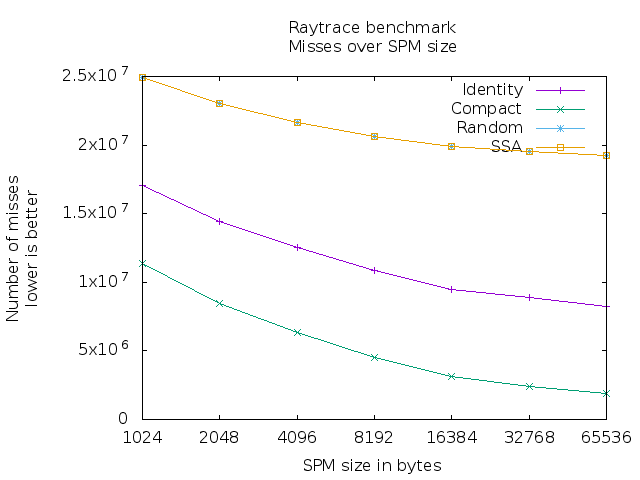
\includegraphics[width = .75\textwidth]{plots/2017-06-13-raytrace-misses.png}
  \caption{Misses of Raytrace benchmark}
  \label{fig:experiment-2017-june-8-raytrace-misses}
\end{figure}

\subsection{Conclusion}
We presented the hypothesis that the memory layout does not matter for scratchpad memories, which know the trace T and liveness intervals of T. For illustrations we discussed a small example which confirms our hypothesis.

In our example, the Belady eviction policy in combination with liveness intervals makes sure that memory accesses and misses remain minimal. The compact allocator only has a chance to get below that number of misses, because it turns a miss into a hit. At allocation time he can immediately achieve this by reusing a dead address in SPM.

To conclude, this small example nicely illustrations that for systems which have certain information about their applications the memory layout has no influence.

\subsection{Further steps}
In this (mini) report we have shown empirically that memory access is constant for all memory layouts. next, we have to prove that a compact allocator as we described in the conclusion is optimal with regards to cache misses in this SPM environment.

\section{27th July, 2017}

\subsection{Experiment: \textit{Bug fix}}
\begin{itemize}
  \item Rerun the experiments of this report, because of the counting bug fix of the LRU caches.
  \item \textit{Expectations:} The number of cycles per instruction for both LRU caches will shrink. Still we expect at both LRU implementations perform worse than OPTCache and BeladyCache.
\end{itemize}

\subsection{Experiment: \textit{Compact-Random-Allocator performance robustness}}
\begin{itemize}
  \item Find a trace optimized for the Compact-Queue-Allocator (Compact-Queue-Allocator performs better than the Compact-Stack-Allocator)
  \item Find a trace optimized for the Compact-Stack-Allocator (Compact-Stack-Allocator performs better than the Compact-Queue-Allocator)
  \item \textit{Expectations:} A good/an interesting result would be if the Compact-Random-Allocator performs (nearly) as good as the Compact-Stack-Allocator, and Compact-Queue-Allocator, respectively.
  \item \textit{Notes}
  \begin{itemize}
    \item 2017-07-31: Right now we think that it is not possible with a free list implementation based on a queue to outperform an stack implementation.
    \begin{itemize}
      \item Either the \textit{most-recently-freed} address is not in the cache anymore, then both implementations force a \textit{cache miss}.
      \item Or the \textit{most-recently-freed} address is still in the cache, then the stack implementation results in a \textit{cache hit} and the queue implementation results in a \textit{cache miss}.
    \end{itemize}
    \item Intuitively by counter-example. Assume high enough associativity. Assume CompactQueue is better than CompactStack in the same situation (same access, same state of free list), i.e. allocation  to address $a$ using CompatQueue results in a cache hit and to address $b$ with CompactStack in a cache miss. Order in free list $a < \dots < b$ and $a \not= b$. Since a free is an access this means that the last access of $a$ was before $b$. Since we have an LRU cache this would imply that $b$ was evicted before $a$, contradicting the access order.
  \end{itemize}
\end{itemize}

\subsection{Experiment: \textit{Associativity influence on LRU caches}}
\begin{itemize}
  \item Pick one of the experiments above, namely Richards.
  \item Pick one fixed cache size 
  \begin{itemize}
    \item either 1024 bytes (very small -> a lot of loads/stores)
    \item or 32KB (more realistic: l1d size of big-iron8 and MacBook Pro)
  \end{itemize}
  \item Run this experiment for different associativities of the LRU caches, e.g, 4, 8, 16, 32, fully
  \item \textit{Expectations:} The number of cycles per instruction should be identical for all associativities of the LRU caches to show that these are independent of the associativity.
\end{itemize}

\subsection{Experiment: \textit{Equally weight stores and loads (cache)}}
\begin{itemize}
  \item Generate some of the performance-indexed-figures with different weight for load and store operations.
  \item Pick two fixed cache sizes, namely 1KB and 64KB.
  \item Pick all 4 experiments from above.
  \item Pick the store-weights as multiples of the load-weights (based on the cache-loads, and cache-stores figures), e.g, 2, 3, 5, 10, ...
  \item \textit{Expectations:} The influence of the store-weight should become recognizable for unrealistic are values. To conclude it is reasonable to weight loads and stores the same.
\end{itemize}

\subsection{Experiment: \textit{Equally weight stores and loads (memory)}}
\begin{itemize}
  \item Same as for the cache loads and stores.
\end{itemize}

\subsection{Experiment: \textit{New benchmarks}}
\begin{itemize}
  \item Find new benchmarks apart of the V8 benchmarks (Richards, Raytrace, Deltablue, and Navier-stroke).
  \item Based on the Scalloc paper try to get access to the SPEC CPU2006 benchmarks.
  \begin{itemize}
    \item Generate traces.
    \item Rerun SemanticLocality with the new traces.
    \item Generate performance-indexed-figures.
  \end{itemize}
  \item \textit{Expectations:} Either confirmation of your previous results or new deep knowledge of the behavior of the caches and allocators, respectively.
\end{itemize}

\section{4th August, 2017}
\subsection{Bubble Pie Chart}

Colors
\begin{itemize}
  \item Hits in green, misses in red
  \item Cache loads, cache store, memory store, memory loads in green, yellow, orange, and red
  \item "Less is better" instead of "Lower is better"
  \item Relative and absolute number of trace reads and writes (= cache stores and loads) in legend of the plot
\end{itemize}

\subsection{Associativity Experiment}
Absolute numbers are enough

\subsection{Line Size}
\begin{itemize}
  \item Try 2 words
  \item A compacting allocator with a \textit{spatial locality threshold} $c$: The allocator remembers the last original address $a$. If a new address for $a+n$ is requested with $n \leq c$, then the allocator looks at the top 2 elements in the free stack and returns the one that is on the same cache line as the address for $a$, or any of the two if there is none.
  \item Change Belady for multi-word lines (next access data structure)
  \item Line size as CLI argument (no range, just a single value)
\end{itemize}

\subsection{Bar chart for number of addresses for all allocators}
Number of different addresses is print as a new column in the experiment results

\subsection{Workload for poor performance of CompactRandom}
\todo{no signs of interests in this direction by Christoph}

\subsection{Description why CompactQueue can never be better than CompactStack}
Intuitively by counter-example. Assume high enough associativity. Assume CompactQueue is better than CompactStack in the same situation (same access, same state of free list), i.e. allocation  to address $a$ using CompatQueue results in a cache hit and to address b with CompactStack in a cache miss. Order in free list $a < \dots < b$ and $a \not= b$. Since $a$ free is an access this means that the last access of $a$ was before $b$. Since we have an LRU cache this would imply that $b$ was evicted before $a$, contradicting the access order.

\todo{copy paste old content}